
% This is a simple template for a LaTeX document using the "article" class.
% See "book", "report", "letter" for other types of document.

\documentclass[10pt]{article} % use larger type; default would be 10pt

\usepackage[T1]{fontenc}
\usepackage[french]{babel}
\usepackage[utf8]{inputenc} % set input encoding (not needed with XeLaTeX)
\usepackage{kpfonts}
\usepackage{hyperref}
\usepackage{listings}

%%% Examples of Article customizations
% These packages are optional, depending whether you want the features they provide.
% See the LaTeX Companion or other references for full information.

%%% PAGE DIMENSIONS
\usepackage{geometry} % to change the page dimensions
\geometry{a4paper} % or letterpaper (US) or a5paper or....
% THE MARGINS FOR DSA is 1.5cm
\geometry{margin=1.5cm} % for example, change the margins to 2 inches all round
% \geometry{landscape} % set up the page for landscape
%   read geometry.pdf for detailed page layout information


% \usepackage[parfill]{parskip} % Activate to begin paragraphs with an empty line rather than an indent

%%% PACKAGES
\usepackage{booktabs} % for much better looking tables
\usepackage{array} % for better arrays (eg matrices) in maths
\usepackage{paralist} % very flexible & customisable lists (eg. enumerate/itemize, etc.)
\usepackage{verbatim} % adds environment for commenting out blocks of text & for better verbatim
% \usepackage{subfig} % make it possible to include more than one captioned figure/table in a single float
% These packages are all incorporated in the memoir class to one degree or another...

%%% HEADERS & FOOTERS
\usepackage{fancyhdr} % This should be set AFTER setting up the page geometry
% \pagestyle{fancy} % options: empty , plain , fancy

\usepackage{graphicx} % support the \includegraphics command and options
\usepackage{subcaption}
\usepackage{caption}

\usepackage{dingbat} % For the pointy hands
\usepackage{pifont}
% \usepackage{xcolor} % For pretty colors
\usepackage[table]{xcolor}
\usepackage{tikz} % for nice pictures
\usepackage{blindtext}
\usepackage{wrapfig}
\usepackage{gensymb}
% \usepackage{table}

% COLORs
\definecolor{mygold}{RGB}{182, 153, 45}
\definecolor{mygreen}{RGB}{62, 171, 0}
\definecolor{dullgreen}{RGB}{165, 181, 45}
\definecolor{mypurp}{RGB}{84, 45, 181}


% \renewcommand{\headrule}{\color{gray}}
\renewcommand{\headrule}{\hbox to\headwidth{%
  \color{gray}\leaders\hrule height \headrulewidth\hfill}}

\renewcommand{\footrulewidth}{1pt}
% \renewcommand{\footrule}{\hbox to\headwirth{
%     \color{gray}\leaders\hrule height \footrulewidth\hfill}}

\renewcommand{\footrule}{{\color{gray}\vskip-\footruleskip\vskip-\footrulewidth \hrule width\headwidth height\footrulewidth\vskip\footruleskip}}

\fancyhf{}
\rhead{\textcolor{gray}{Séance TP 1}}
\chead{\color{gray} Travaux Pratiques}
% \lhead{Optimisation du GCC}
\lfoot{\color{gray}\textcopyright 2022 Evan Voyles}
\rfoot{\color{gray} Page \thepage\ sur 3}
\cfoot{\color{gray}Spécialité MAIN-3}
\footskip = 0pt
% \voffset = 10pt
% \headsep = 0pt
% \cfoot{\thepage\ of \pageref{LastPage}}

% \renewcommand{\headrulewidth}{0pt} % customise the layout...
% \lhead{}\chead{}\rhead{}
% \lfoot{}\cfoot{\thepage}\rfoot{}


\usepackage[absolute,overlay]{textpos} % Add text in any arbitrary position

%%% SECTION TITLE APPEARANCE
\usepackage{sectsty}
\allsectionsfont{\sffamily\mdseries\upshape} % (See the fntguide.pdf for font help)
% (This matches ConTeXt defaults)

%%% ToC (table of contents) APPEARANCE
\usepackage[nottoc,notlof,notlot]{tocbibind} % Put the bibliography in the ToC
\usepackage[titles,subfigure]{tocloft} % Alter the style of the Table of Contents
\renewcommand{\cftsecfont}{\rmfamily\mdseries\upshape}
\renewcommand{\cftsecpagefont}{\rmfamily\mdseries\upshape} % No bold!

%%% END Article customizations

%%% The "real" document content comes below...

\newcommand{\asgold}[1]{\textcolor{mygold}{{\bf#1}}}
\newcommand{\asgrey}[1]{\textcolor{gray}{{\bf#1}}}
\newcommand{\asred}[1]{\textcolor{red}{{\bf#1}}}
\newcommand{\asor}[1]{\textcolor{orange}{{\bf#1}}}
\newcommand{\ascy}[1]{\textcolor{cyan}{{\bf#1}}}
\newcommand{\asgr}[1]{\textcolor{mygreen}{{\bf#1}}}
\newcommand{\aspurp}[1]{\textcolor{mypurp}{{\bf#1}}}


\begin{document}

% \vspace{-10pt}
% This is the PERFECT SCALING, now we need to adjust the scale a little bit.
\begin{tikzpicture}[remember picture,overlay,yshift=-.2cm, xshift=1.75cm] % LMAOOOOOO This is the EXACT POSITION!!!!
    \node at (0,0) {
\includegraphics[width=4.0cm,height=1.6cm]{media/1280px-Logo_Polytech_Sorbonne.png}};
\end{tikzpicture}

% \hspace{-5cm}
% \hspace{-1cm}
% \hspace{-1cm}

\vspace{-1cm}
\vspace{0.3cm}

{\raggedleft \color{mygold} Algorithmique générale\\
MAIN-3, année 2022\\
Séance TP N\degree 1\\
Février 2022\\
VOYLES Evan\\}

% This vspace accomodates my name
\vspace{-0.42cm}
\vspace{1.23cm}

{\Large \noindent \color{mygold} Objectif}

{\color{mygold}\noindent\rule{\textwidth}{1pt}}
\vspace{0cm}
\begin{itemize}
    \item[{\color{mygold}\ding{43}}] Complexité en moyenne.
\end{itemize}

\vspace{1.2cm}
{\color{dullgreen}\noindent \Large \bf Problème}

\vspace{-0.28cm}
{\vspace{0cm}\color{dullgreen}\noindent\rule{\textwidth}{1pt}}

\begin{textblock*}{10cm}(9.9cm,7.2cm) % {block width} (coords)
    \Large \aspurp{[Complexité en moyenne du tri rapide]}
\end{textblock*}

\begin{enumerate}
    % \item Réaliser un suivi à la trace de la procédure \verb|partitionBis| appliquée aux instances suivantes :
    \item Réaliser un suivi à la trace de la procédure \texttt{partitionBis} appliquée aux instances suivantes :
    \begin{equation*}
        I_1 = [2,6,0,4,3,1,5], I_2 = [7,6,5,4,3,2,1]\ \ \mathrm{ et }\ \ I_3 = [1,2,3,4,5,6,7].
    \end{equation*}
\end{enumerate}

% \newpage


% Test out a table!!!
\begin{table}[h!]
    \begin{tabular}{ll|ccccc}
    \hline
    Instruction                    & Description/Remarque                                          & T                         & indpiv & pospiv & x & j \\
    \hline
    partitionBis(I$_1$, 0, 6)      & \asgold{T \textless{}- I$_1$},  deb \textless{}- 0, fin \textless{}- 6 & \asgold{{[}2, 6, 0, 4, 3, 1, 5{]}} &        &        &   &   \\
    indpiv \textless{}- deb        &       \asgold{indipiv \textless{}- 0}                                                       & {[}2, 6, 0, 4, 3, 1, 5{]} & \asgold{0}      &        &   &   \\
    pospiv \textless{}- deb      &           \asgold{pospiv \textless{}- 0}                                                    & {[}2, 6, 0, 4, 3, 1, 5{]} & 0      & \asgold{0}      &   &   \\
    x \textless{}- T(deb)            &        \asgold{x \textless{}- T(0)}                                                       & {[}2, 6, 0, 4, 3, 1, 5{]} & 0      & 0      & \asgold{2} &   \\
    \asgr{[Pour]} j \textless{}- deb + 1  & \asgold{j \textless{}- 0 + 1}                                                              & {[}2, 6, 0, 4, 3, 1, 5{]} & 0      & 0      & 2 & \asgold{1} \\
    \asgr{[Pour]} j \textless{}= fin      & \aspurp{1 \textless{}= 6} est vrai, la boucle continue                    & {[}2, 6, 0, 4, 3, 1, 5{]} & 0      & 0      & 2 & \aspurp{1} \\
    \asgr{\ \ \ [Si]\ \ } T(j) \textless{}= x       & \cellcolor{mypurp} 6 \textless{}= 2 est faux, on retourne a la boucle            & {[}\aspurp{2}, \aspurp{6}, 0, 4, 3, 1, 5{]} & 0      & 0      & 2 & 1 \\
    \asgr{[Pour]} j \textless{}- j + 1   &  \asgold{j \textless{} - 1 + 1}                            & {[}2, 6, 0, 4, 3, 1, 5{]} & 0      & 0      & 2 & \asgold{2} \\
    \asgr{[Pour]} j \textless{}= fin      & \aspurp{2 \textless{}= 6} est vrai, la boucle continue                 & {[}2, 6, 0, 4, 3, 1, 5{]} & 0      & 0      & 2 & 2 \\
    \asgr{\ \ \ [Si]\ \ } T(j) \textless{}= x       & \cellcolor{mypurp} 0 \textless{}= 2 est vrai                                     & {[}\aspurp{2}, 6, \aspurp{0}, 4, 3, 1, 5{]} & 0      & 0      & 2 & 2 \\
    pospiv \textless{}- pospiv + 1 &         \asgold{pospiv \textless{}- 0 + 1}                                                      & {[}2, 6, 0, 4, 3, 1, 5{]} & 0      & \asgold{1}      & 2 & 2 \\
    \asgr{\ \ \ [Si]\ \ } j \textgreater pospiv     & \aspurp{2 \textgreater{}} 1 est vrai                                     & {[}2, 6, 0, 4, 3, 1, 5{]} & 0      & 1      & 2 & 2 \\
    echanger(T, pospiv, j)         &  \cellcolor{mygold}T(1) \textless{}- 0, T(2) \textless{}- 6                                         & {[}2, \asgold{0}, \asgold{6}, 4, 3, 1, 5{]} & 0      & 1      & 2 & 2 \\
    \asgr{[Pour]} j \textless{}- j + 1   &  \asgold{j \textless{} - 2 + 1}                             & {[}2, 0, 6, 4, 3, 1, 5{]} & 0      & 1      & 2 & \asgold{3} \\
    \asgr{[Pour]} j \textless{}= fin      & \aspurp{3 \textless{}= 6} est vrai, la boucle continue                 & {[}2, 0, 6, 4, 3, 1, 5{]} & 0      & 1      & 2 & 3 \\
    \asgr{\ \ \ [Si]\ \ } T(j) \textless{}= x       & \cellcolor{mypurp} 4 \textless{}= 2 est faux                                     & {[}\aspurp{2}, 0, 6, \aspurp{4}, 3, 1, 5{]} & 0      & 1      & 2 & 3 \\
    \asgr{[Pour]} j \textless{}- j + 1   &  \asgold{j \textless{} - 3 + 1}                             & {[}2, 0, 6, 4, 3, 1, 5{]} & 0      & 1      & 2 & \asgold{4} \\
    \asgr{[Pour]} j \textless{}= fin      & \aspurp{4 \textless{}= 6} est vrai, la boucle continue                 & {[}2, 0, 6, 4, 3, 1, 5{]} & 0      & 1      & 2 & 4 \\
    \asgr{\ \ \ [Si]\ \ } T(j) \textless{}= x       & \cellcolor{mypurp} 3 \textless{}= 2 est faux                                     & {[}\aspurp{2}, 0, 6, 4, \aspurp{3}, 1, 5{]} & 0      & 1      & 2 & 4 \\
    \asgr{[Pour]} j \textless{}- j + 1   &  \asgold{j \textless{} - 4 + 1}                             & {[}2, 0, 6, 4, 3, 1, 5{]} & 0      & 1      & 2 & \asgold{5} \\
    \asgr{[Pour]} j \textless{}= fin      & \aspurp{5 \textless{}= 6} est vrai, la boucle continue                 & {[}2, 0, 6, 4, 3, 1, 5{]} & 0      & 1      & 2 & 5 \\
    \asgr{\ \ \ [Si]\ \ } T(j) \textless{}= x       & \cellcolor{mypurp} 1 \textless{}= 2 est vrai                                     & {[}\aspurp{2}, 0, 6, 4, 3, \aspurp{1}, 5{]} & 0      & 1      & 2 & 5 \\
    pospiv \textless{}- pospiv + 1 &      \asgold{pospiv \textless{}- 1 + 1}                                                         & {[}2, 0, 6, 4, 3, 1, 5{]} & 0      & \asgold{2}      & 2 & 5 \\
    \asgr{\ \ \ [Si]\ \ } j \textgreater pospiv     & \aspurp{5 \textgreater{} 2} est vrai                                     & {[}2, 0, 6, 4, 3, 1, 5{]} & 0      & 2      & 2 & 5 \\
    echanger(T, pospiv, j)         & \cellcolor{mygold}T(2) \textless{}- 1, T(5) \textless{}- 6                                         & {[}2, 0, \asgold{1}, 4, 3, \asgold{6}, 5{]} & 0      & 2      & 2 & 5 \\
    \asgr{[Pour]} j \textless{}- j + 1   &  \asgold{j \textless{} - 5 + 1}                             & {[}2, 0, 1, 4, 3, 6, 5{]} & 0      & 2      & 2 & \asgold{6} \\
    \asgr{[Pour]} j \textless{}= fin      & \aspurp{6 \textless{}= 6} est vrai, la boucle continue               & {[}2, 0, 1, 4, 3, 6, 5{]} & 0      & 2      & 2 & 6 \\
    \asgr{\ \ \ [Si]\ \ } T(j) \textless{}= x       & \cellcolor{mypurp} 5 \textless{}= 2 est faux                                     & {[}\aspurp{2}, 0, 1, 4, 3, 6, \aspurp{5}{]} & 0      & 2      & 2 & 6 \\
    \asgr{[Pour]} j \textless{}- j + 1   &  \asgold{j \textless{} - 6 + 1}                             & {[}2, 0, 1, 4, 3, 6, 5{]} & 0      & 2      & 2 & \asgold{7} \\
    \asgr{[Pour]} j \textless{}= fin      & \aspurp{7 \textless{}= 6} est faux, la boucle termine                   & {[}2, 0, 1, 4, 3, 6, 5{]} & 0      & 2      & 2 & \aspurp{7} \\
    \asgr{\ \ \ [Si]\ \ } indpiv \textless{} pospiv   & \aspurp{0 \textless{} 2} est vrai                                        & {[}2, 0, 1, 4, 3, 6, 5{]} & 0      & 2      & 2 & 7 \\
    echanger(T, indpiv, pospiv)    &  \cellcolor{mygold}T(0) \textless{}- 1, T(2) \textless{}- 2                                        & {[}\asgold{1}, 0, \asgold{2}, 4, 3, 6, 5{]} & 0      & 2      & 2 & 7 \\
    \hline
    \end{tabular}
    \end{table}

\vspace{-0.4cm}
\noindent Nombre d'\asgold{échanges} : 3, Nombre de \aspurp{comparaison} : 6

\vspace{0.2cm}
Notre tableau en sorti $[1, 0, \asred{2}, 4, 3, 6, 4]$ a été partitionné en deux parties autour du pivot $\asred{2}$. A gauche, l'on a $T_g = [1, 0]$ dont tous
les éléments $g \in T_g$ satisfaitent $g < \asred{2}$ et à droite l'on a $T_d = [4, 3, 6, 5] \mid \forall d \in T_d,\ d > \asred{2}$. La schéma de partition de
l'algorithme \texttt{partitionBis} parcours le tableau pour compter le nombre des valeurs qui sont inférieures au pivot. En le comptant, s'il il y a des
valuers plus grand que le pivot dans le soustableau à gauche, \texttt{partitionBis} va effectuer un échange. Donc, on verra que ce schéma doit opérer $n - 1$ comparaisons
des éléments du tableau à trier.

\newpage

\pagestyle{fancy}

% Test out a table!!!
\begin{table}[h!]
    \begin{tabular}{ll|ccccc}
    \hline
    % \rowcolor{red} Instruction                    & Description/Remarque                                          & T                         & indpiv & pospiv & x & j \\
    % \rowcolor{mygold}
    Instruction                    & Description/Remarque                                          & T                         & indpiv & pospiv & x & j \\
    \hline
    partitionBis(I$_2$, 0, 6)    & \asgold{T \textless{}- I$_2$},  deb \textless{}- 0, fin \textless{}- 6 & \asgold{{[}7, 6, 5, 4, 3, 2, 1{]}} &        &        &   &   \\
    indpiv \textless{}- deb      & \asgold{indpiv \textless{}- 0}                                                            & {[}7, 6, 5, 4, 3, 2, 1{]} & \asgold{0}      &        &   &   \\
    pospiv \textless{}- deb      & \asgold{pospiv \textless{}- 0}                                                             & {[}7, 6, 5, 4, 3, 2, 1{]} & 0      & \asgold{0}      &   &   \\
    x \textless{}- T(deb)            &        \asgold{x \textless{}- 7}                             & {[}7, 6, 5, 4, 3, 2, 1{]} & 0      & 0      & \asgold{7} &   \\
    \asgr{[Pour]} j \textless{}- deb + 1  &  \asgold{j \textless{}- 0 + 1}                                                              & {[}7, 6, 5, 4, 3, 2, 1{]} & 0      & 0      & 7 & \asgold{1} \\
    \asgr{[Pour]} j \textless{}= fin      & \aspurp{1 \textless{}= 6} est vrai, la boucle continue                 & {[}7, 6, 5, 4, 3, 2, 1{]} & 0      & 0      & 7 & \aspurp{1} \\
    \asgr{\ \ \ [Si]\ \ } T(j) \textless{}= x       & \cellcolor{mypurp} 6 \textless{}= 7 est vrai                                     & {[}\aspurp{7}, \aspurp{6}, 5, 4, 3, 2, 1{]} & 0      & 0      & 7 & 1 \\
    pospiv \textless{}- pospiv + 1 & \asgold{pospiv \textless{}- 0 + 1}                                            & {[}7, 6, 5, 4, 3, 2, 1{]} & 0      & \asgold{1}      & 7 & 1 \\
    \asgr{\ \ \ [Si]\ \ } j \textgreater{} pospiv     & \aspurp{1 \textgreater{} 1} est faux                                     & {[}7, 6, 5, 4, 3, 2, 1{]} & 0      & \aspurp{1}      & 7 & \aspurp{1} \\
    \asgr{[Pour]} j \textless{}- j + 1  &  \asgold{j \textless{}- 1 + 1}                                                              & {[}7, 6, 5, 4, 3, 2, 1{]} & 0      & 1      & 7 & \asgold{2} \\
    \asgr{[Pour]} j \textless{}= fin      & \aspurp{2 \textless{}= 6} est vrai, la boucle continue                 & {[}7, 6, 5, 4, 3, 2, 1{]} & 0      & 1      & 7 & \aspurp{2} \\
    \asgr{\ \ \ [Si]\ \ } T(j) \textless{}= x       & \cellcolor{mypurp} 5 \textless{}= 7 est vrai                                     & {[}\aspurp{7}, 6, \aspurp{5}, 4, 3, 2, 1{]} & 0      & 1      & 7 & 2 \\
    pospiv \textless{}- pospiv + 1  & \asgold{pospiv \textless{}- 1 + 1}               & {[}7, 6, 5, 4, 3, 2, 1{]} & 0      & \asgold{2}      & 7 & 2 \\
    \asgr{\ \ \ [Si]\ \ } j \textgreater{} pospiv     & \aspurp{2 \textgreater{} 2} est faux                                     & {[}7, 6, 5, 4, 3, 2, 1{]} & 0      & \aspurp{2}      & 7 & \aspurp{2} \\
    \asgr{[Pour]} j \textless{}- j + 1  &        \asgold{j \textless{}- 2 + 1}                                                        & {[}7, 6, 5, 4, 3, 2, 1{]} & 0      & 2      & 7 & \asgold{3} \\
    \asgr{[Pour]} j \textless{}= fin      & \aspurp{3 \textless{}= 6} est vrai, la boucle continue                 & {[}7, 6, 5, 4, 3, 2, 1{]} & 0      & 2      & 7 & \aspurp{3} \\
    \asgr{\ \ \ [Si]\ \ } T(j) \textless{}= x       & \cellcolor{mypurp} 4 \textless{}= 7 est vrai                                     & {[}\aspurp{7}, 6, 5, \aspurp{4}, 3, 2, 1{]} & 0      & 2      & 7 & 3 \\
    pospiv \textless{}- pospiv + 1  & \asgold{pospiv \textless{}- 2 + 1}               & {[}7, 6, 5, 4, 3, 2, 1{]} & 0      & \asgold{3}      & 7 & 3 \\
    \asgr{\ \ \ [Si]\ \ } j \textgreater{} pospiv     & \aspurp{3 \textgreater{} 3} est faux                                     & {[}7, 6, 5, 4, 3, 2, 1{]} & 0      & \aspurp{3}      & 7 & \aspurp{3} \\
    \asgr{[Pour]} j \textless{}- j + 1  &          \asgold{j \textless{}- 3 + 1}                                                      & {[}7, 6, 5, 4, 3, 2, 1{]} & 0      & 3      & 7 & \asgold{4} \\
    \asgr{[Pour]} j \textless{}= fin      & \aspurp{4 \textless{}= 6} est vrai, la boucle continue                 & {[}7, 6, 5, 4, 3, 2, 1{]} & 0      & 3      & 7 & \aspurp{4} \\
    \asgr{\ \ \ [Si]\ \ } T(j) \textless{}= x       & \cellcolor{mypurp} 3 \textless{}= 7 est vrai                                     & {[}\aspurp{7}, 6, 5, 4, \aspurp{3}, 2, 1{]} & 0      & 3      & 7 & 4 \\
    pospiv \textless{}- pospiv + 1  & \asgold{pospiv \textless{}- 3 + 1}               & {[}7, 6, 5, 4, 3, 2, 1{]} & 0      & \asgold{4}      & 7 & 4 \\
    \asgr{\ \ \ [Si]\ \ } j \textgreater{} pospiv     & \aspurp{4 \textgreater{} 4} est faux                                     & {[}7, 6, 5, 4, 3, 2, 1{]} & 0      & \aspurp{4}      & 7 & \aspurp{4} \\
    \asgr{[Pour]} j \textless{}- j + 1  &             \asgold{j \textless{}- 4 + 1}                                                   & {[}7, 6, 5, 4, 3, 2, 1{]} & 0      & 4      & 7 & \asgold{5} \\
    \asgr{[Pour]} j \textless{}= fin      & \aspurp{5 \textless{}= 6} est vrai, la boucle continue                 & {[}7, 6, 5, 4, 3, 2, 1{]} & 0      & 4      & 7 & \aspurp{5} \\
    \asgr{\ \ \ [Si]\ \ } T(j) \textless{}= x       & \cellcolor{mypurp} 2 \textless{}= 7 est vrai                                     & {[}\aspurp{7}, 6, 5, 4, 3, \aspurp{2}, 1{]} & 0      & 4      & 7 & 5 \\
    pospiv \textless{}- pospiv + 1  & \asgold{pospiv \textless{}- 4 + 1}               & {[}7, 6, 5, 4, 3, 2, 1{]} & 0      & \asgold{5}      & 7 & 5 \\
    \asgr{\ \ \ [Si]\ \ } j \textgreater{} pospiv     & \aspurp{5 \textgreater{} 5} est faux                                     & {[}7, 6, 5, 4, 3, 2, 1{]} & 0      & \aspurp{5}      & 7 & \aspurp{5} \\
    \asgr{[Pour]} j \textless{}- j + 1  &           \asgold{j \textless{}- 5 + 1}                                                     & {[}7, 6, 5, 4, 3, 2, 1{]} & 0      & 5      & 7 & \asgold{6} \\
    \asgr{[Pour]} j \textless{}= fin      & \aspurp{6 \textless{}= 6} est vrai, la boucle continue                 & {[}7, 6, 5, 4, 3, 2, 1{]} & 0      & 5      & 7 & \aspurp{6} \\
    \asgr{\ \ \ [Si]\ \ } T(j) \textless{}= x       & \cellcolor{mypurp} 1 \textless{}= 7 est vrai                                     & {[}\aspurp{7}, 6, 5, 4, 3, 2, \aspurp{1}{]} & 0      & 5      & 7 & 6 \\
    pospiv \textless{}- pospiv + 1  & \asgold{pospiv \textless{}- 5 + 1}               & {[}7, 6, 5, 4, 3, 2, 1{]} & 0      & \asgold{6}      & 7 & 6 \\
    \asgr{\ \ \ [Si]\ \ } j \textgreater{} pospiv     & \aspurp{5 \textgreater{} 5} est faux                                     & {[}7, 6, 5, 4, 3, 2, 1{]} & 0      & \aspurp{6}      & 7 & \aspurp{6} \\
    \asgr{[Pour]} j \textless{}- j + 1  &           \asgold{j \textless{}- 6 + 1}                                                     & {[}7, 6, 5, 4, 3, 2, 1{]} & 0      & 6      & 7 & \asgold{7} \\
    \asgr{[Pour]} j \textless{}= fin      & \aspurp{7 \textless{}= 6} est faux, la boucle termine                   & {[}7, 6, 5, 4, 3, 2, 1{]} & 0      & 6      & 7 & \aspurp{7} \\
    \asgr{\ \ \ [Si]\ \ } indpiv \textless{} pospiv   & \aspurp{0 \textless{} 6} est vrai                                        &  {[}7, 6, 5, 4, 3, 2, 1{]} & \aspurp{0}      & \aspurp{6}      & 7 & 7 \\
    echanger(T, indpiv, pospiv)    & \cellcolor{mygold} T(0) \textless{}- 1, T(6) \textless{}- 7                                        &  {[}\asgold{1}, 6, 5, 4, 3, 2, \asgold{7}{]}  & 0      & 6      & 7 & 7 \\
    \hline
    \end{tabular}
    \end{table}

\vspace{-.4cm}
\noindent Nombre d'\asgold{échanges} : 1, Nombre de \aspurp{comparaison} : 6

\vspace{0.2cm}
Chaque élément du tableau qu'on à comparé avec le pivot en était inférieur. Cependant, on a réussi a partitionner le tableau avec un
seul échange dans le dernier étape. Avec le pivot $\asred{7}$, $T_g = [1, 6, 5, 4, 3, 2]$ et il vérifie $g < \asred{7}\ \forall g \in T_g$.

\newpage

% Third table!!!!
\begin{table}[h!]
    \begin{tabular}{ll|ccccc}
    \hline
    % \rowcolor{red} Instruction                    & Description/Remarque                                          & T                         & indpiv & pospiv & x & j \\
    % \rowcolor{mygold}
    Instruction                    & Description/Remarque                                          & T                         & indpiv & pospiv & x & j \\
    \hline
    partitionBis(I$_3$, 0, 6)    & \asgold{T \textless{}- I$_3$},  deb \textless{}- 0, fin \textless{}- 6 & \asgold{{[}1, 2, 3, 4, 5, 6, 7{]}} &        &        &   &   \\
    indpiv \textless{}- deb      & \asgold{indpiv \textless{}- 0}                                                            & {[}1, 2, 3, 4, 5, 6, 7{]} & \asgold{0}      &        &   &   \\
    pospiv \textless{}- deb      & \asgold{pospiv \textless{}- 0}                                                             & {[}1, 2, 3, 4, 5, 6, 7{]} & 0      & \asgold{0}      &   &   \\
    x \textless{}- T(deb)            &        \asgold{x \textless{}- 1}                             & {[}1, 2, 3, 4, 5, 6, 7{]} & 0      & 0      & \asgold{1} &   \\
    \asgr{[Pour]} j \textless{}- deb + 1  &  \asgold{j \textless{}- 0 + 1}                                                              & {[}1, 2, 3, 4, 5, 6, 7{]} & 0      & 0      & 1& \asgold{1} \\
    \asgr{[Pour]} j \textless{}= fin      & \aspurp{1 \textless{}= 6} est vrai, la boucle continue                 & {[}1, 2, 3, 4, 5, 6, 7{]} & 0      & 0      & 1& \aspurp{1} \\
    \asgr{\ \ \ [Si]\ \ } T(j) \textless{}= x       & \cellcolor{mypurp} 2 \textless{}= 1 est faux & {[}\aspurp{1}, \aspurp{2}, 3, 4, 5, 6, 7{]} & 0      & 0      & 1& 1 \\
    \asgr{[Pour]} j \textless{}- j + 1  &  \asgold{j \textless{}- 1 + 1}                                                              & {[}1, 2, 3, 4, 5, 6, 7{]} & 0      & 0      & 1& \asgold{2} \\
    \asgr{[Pour]} j \textless{}= fin      & \aspurp{2 \textless{}= 6} est vrai, la boucle continue                 & {[}1, 2, 3, 4, 5, 6, 7{]} & 0      & 0      & 1& \aspurp{2} \\
    \asgr{\ \ \ [Si]\ \ } T(j) \textless{}= x       & \cellcolor{mypurp} 3 \textless{}= 1 est faux                                     & {[}\aspurp{1}, 2, \aspurp{3}, 4, 5, 6, 7{]} & 0      & 0      & 1& 2 \\

    \asgr{[Pour]} j \textless{}- j + 1  &  \asgold{j \textless{}- 2 + 1}                                                              & {[}1, 2, 3, 4, 5, 6, 7{]} & 0      & 0      & 1& \asgold{3} \\
    \asgr{[Pour]} j \textless{}= fin      & \aspurp{3 \textless{}= 6} est vrai, la boucle continue                 & {[}1, 2, 3, 4, 5, 6, 7{]} & 0      & 0      & 1& \aspurp{3} \\
    \asgr{\ \ \ [Si]\ \ } T(j) \textless{}= x       & \cellcolor{mypurp} 4 \textless{}= 1 est faux                                     & {[}\aspurp{1}, 2, 3, \aspurp{4}, 5, 6, 7{]} & 0      & 0      & 1& 3 \\
    \asgr{[Pour]} j \textless{}- j + 1  &  \asgold{j \textless{}- 3 + 1}                                                              & {[}1, 2, 3, 4, 5, 6, 7{]} & 0      & 0      & 1& \asgold{4} \\
    \asgr{[Pour]} j \textless{}= fin      & \aspurp{4 \textless{}= 6} est vrai, la boucle continue                 & {[}1, 2, 3, 4, 5, 6, 7{]} & 0      & 0      & 1& \aspurp{4} \\
    \asgr{\ \ \ [Si]\ \ } T(j) \textless{}= x       & \cellcolor{mypurp} 5 \textless{}= 1 est faux                                     & {[}\aspurp{1}, 2, 3, 4, \aspurp{5}, 6, 7{]} & 0      & 0      & 1& 4 \\
    \asgr{[Pour]} j \textless{}- j + 1  &  \asgold{j \textless{}- 4 + 1}                                                              & {[}1, 2, 3, 4, 5, 6, 7{]} & 0      & 0      & 1& \asgold{5} \\
    \asgr{[Pour]} j \textless{}= fin      & \aspurp{5 \textless{}= 6} est vrai, la boucle continue                 & {[}1, 2, 3, 4, 5, 6, 7{]} & 0      & 0      & 1& \aspurp{5} \\
    \asgr{\ \ \ [Si]\ \ } T(j) \textless{}= x       & \cellcolor{mypurp} 6 \textless{}= 1 est faux                                     & {[}\aspurp{1}, 2, 3, 4, 5, \aspurp{6}, 7{]} & 0      & 0      & 1& 5 \\
    \asgr{[Pour]} j \textless{}- j + 1  &  \asgold{j \textless{}- 5 + 1}                                                              & {[}1, 2, 3, 4, 5, 6, 7{]} & 0      & 0      & 1& \asgold{6} \\
    \asgr{[Pour]} j \textless{}= fin      & \aspurp{6 \textless{}= 6} est vrai, la boucle continue                   & {[}1, 2, 3, 4, 5, 6, 7{]} & 0      & 0      & 1 & \aspurp{6} \\
    \asgr{\ \ \ [Si]\ \ } T(j) \textless{}= x       & \cellcolor{mypurp} 7 \textless{}= 1 est faux                                     & {[}\aspurp{1}, 2, 3, 4, 5, 6, \aspurp{7}{]} & 0      & 0      & 1& 6 \\
    \asgr{[Pour]} j \textless{}- j + 1  &  \asgold{j \textless{}- 6 + 1}                                                              & {[}1, 2, 3, 4, 5, 6, 7{]} & 0      & 0      & 1& \asgold{7} \\
    \asgr{[Pour]} j \textless{}= fin      & \aspurp{7 \textless{}= 6} est faux, la boucle termine                   & {[}1, 2, 3, 4, 5, 6, 7{]} & 0      & 0      & 1 & \aspurp{7} \\
    \asgr{\ \ \ [Si]\ \ } indpiv \textless{} pospiv   & \aspurp{0 \textless{} 0} est faux &  {[}1, 2, 3, 4, 5, 6, 7{]} & \aspurp{0}      & \aspurp{0}      & 1 & 7 \\
    \hline
    \end{tabular}
    \end{table}

\vspace{-.4cm}
\noindent Nombre d'\asgold{échanges} : 0, Nombre de \aspurp{comparaison} : 6
% \newpage

% \vspace{0.2cm}
Tous les éléments de $I_3 = [1, 2, 3, 4, 5, 6, 7]$ sont déjà triés donc on effectue aucun échange. On constate qu'il y a encore $n - 1 = 6$ comparaisons parce qu'on a
traversé le tableau à partir du premier élément jusqu'a l'avant-dernier élément. Le tableau est, bien entendu, bien partitionné autor $p = \asred{1}$, tel que $T_d = [2, 3, 4, 5, 6, 7]$.


\begin{itemize}
    \item[2.] Démontrer que la procédure \texttt{partitionBis} est correcte et analyser sa complexité.
\end{itemize}

Pour démontrer que la procédure \texttt{partitionBis} est correcte on doit prouver que donné n'importe quel
instance, l'algorithme \texttt{partitionBis} renvoie un tableau qui est partitionné. Pour procéder, on définit donc un tableau
partitionné est celui dont tous les éléments à gauche d'un élément dit pivot est inférieure au pivot, et tout élément à droite
du pivot est supérieure au pivot. Afin d'analyser si le programme est correcte ou pas, on va s'orienter autour de deux questions principales: Est-ce que l'élément qu'on a
choisit d'être le pivot finit d'être dans la bonne place ? Si oui, est-ce que tous les éléments à gauche sont inférieurs au pivot et respectivement supérieurs pour les éléments à
droite. Commen\c cons avec la question de la position du pivot.

Si on observe notre suivie à la trace pour les trois instances, on voit que l'algorithme parcours le tableau à partir du deuxième élément (le premier est choisi pour être le pivot),
jusqu'à la fin. Si la valeur qu'on visite est inférieur au pivot, on incrémente \texttt{pospiv}. En effet, on parcours le tableau et on compte le nombre d'éléments qui sont inférieurs au pivot.
En d'autre termes, on compte le nombre de valeurs qui doivent être à gauche du pivot dans la configuration finale. Pour prouver que le pivot se trouve \textit{toujours} dans la bonne place, on considère
l'effet de la dernière condition \texttt{if}. La condition est: Si indpiv < pospiv, échange le pivot avec l'élément à T(pospiv). Il n'est pas évident mais avec un peu de reflexion on raisonne que indpiv
reste 0 pendant l'exécution de l'algorithme, donc le seule fois où cette condition n'est pas satisfaite c'est si pospiv n'est jamais incrémenté. Quand est-ce que cela se passe ? On a vu que pour l'instance
$I_3$, il n'y a aucun élément entre $T(1)$ et $T(fin)$ qui est moins que le pivot, 1. Donc, la condition $T(j)$ n'est jamais satisfaite et du coup on incrémente jamais la variable pospiv.
Comme 0 < 0 est faux, on fais pas bouger le pivot quand il est deja à la bonne position. Comme on choisi le premier élément pour chaque appel à \texttt{partitionBis}, on effectue un échange du pivot si et seulement si
il n'est pas dans la bonne place. Et donc, où est-ce qu'on fait bouger le pivot si cette condition est vérifiée ? On le met à T(pospiv), la position dans le tableau avec pospiv éléments à gauche, qu'on va démontrer qu'ils sont
tous inférieurs au pivot. Par conséquent, la procédure \texttt{partitionBis} assure que le pivot finit toujours dans la bonne position.

Procédons pour démontrer que tous les éléments à gauche du pivot sont inférieurs au pivot. Pour ce faire, on considère la fonctionnement des phrases \texttt{if}
à l'intérieur de la boucle principale. Si l'élément qu'on visite est inférieur au pivot, on incrémente \texttt{pospiv} et on teste une autre condition. Si j > pospiv,
on effectue un échange. Digérons qu'est-ce que ces branches de logiques font. Quand est-ce que cette condition n'est pas vérifié? Comme j incrémente à chaque itération,
cette condition n'est pas vérifié si pospiv est égale a j. Cela se passe si on incrémente pospiv à chaque fois, ce qui se passe seulement quand la valeur qu'on visite est plus petite
que le pivot. Donc, à chaque fois qu'on teste cette condition, il est vérifé s'il y a au moins un élément qu'on à visité qui est inférieur au pivot.

Pensons comment \c ca s'applique aux instances au-dessus. pour $I_2$, chaque élément que l'on visite est inférieur au pivot, du coup pospiv est toujours égale à j et la
condition nécessaire pour échanger deux éléments est fausse. On effectue donc aucun échange jusqu'au dernière condition où on teste si il ya des éléments inférieurs au pivot.
Comme il y'en a 6, on fait un seul échange pour mettre le pivot à la bonne place, ce qu'on a discuté en haut. Ca c'est le cas où tous les éléments sont inférieus au pivot, donc
on incrémente pospiv à chaque fois et donc on fait aucun échange dans la boucle principale. Si on reflichit à ce qui se passe avec $I_1$, des qu'il y à un élément qui est plus petit
que le pivot et qu'on a déjà visité un élément plus grand, on effectue un échange pour mettre celui qui est plus petit à gauche de la position finale. Comme cela, lorsqu'on parcours le
tableau, on mets les valuers inférieures au pivot à gauche.

L'algorithme donc satisfait les deux conditions pour tous les instances - que le pivot soit dans la bonne place et que tous les éléments à gauche sont inférieurs au pivot; tous les éléments à
droite du pivot sont supérieurs, et par définition il est correcte.


\begin{itemize}
    \item[3.] Quels changements, s'ils existent, à apporter au pseudo-code du tri rapide?
\end{itemize}

La valeur de sortie de la procédure \texttt{partitionBis} est exactement la même chose que pour \texttt{partition} parce que toutes les deux renvoient
l'indice de la position finale de l'élément choisit comme le pivot. Si on donne en entrée le même tableau et on choisit le même élément comme pivot, on renvoie la même
position finale. Donc, le seul changement que l'on doit apporter au pseudo-code du tri rapide est
de changer la ligne 10 pour affecter le résultat de \texttt{partitionBis(T, deb, fin)} à $\pi$, au lieu de lui affecter le résultat de \texttt{partition}.
Pour être clair, à la place d'appeler la procédure \texttt{partition} afin de partitionner notre tableau, on choisit le schématique de \texttt{partitionBis}.

\begin{itemize}
    \item[4.] Conduire une analyse de complexité en moyenne du tri rapide utilisant la procédure \texttt{partitionBis} à la
    place de la procédure \texttt{partition}.
\end{itemize}

Commen\c cons l'analyse de complexité de la procédure \texttt{partitionBis} en étudiant la moyenne du nombre de comparaisons
pour trier $m$ tableau de taille $n$ dont les éléments sont $\{ 0, 1, ..., n - 1\}$ mélangés selon le battage de Fisher-Yates.
Fixons $m = 100$ et $n = \{10, 50, 110, ..., 4950\}$ Il est facile à comptabiliser le nombre de comparaisons $\mu_{cmp}$ pour exécuter le tri rapide avec
le schéma de partition \texttt{partitionBis}. Pour ce faire, on observe qu'il y a un comparaison chaque passage du boucle. Donc,
on écrit le code suivant en C

\begin{figure}[h!]
    \centering
    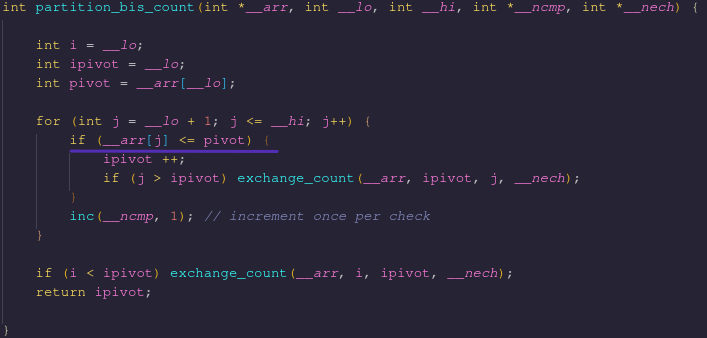
\includegraphics[width=.7\linewidth]{./media/partition_bis_count.png}
    \caption{Définition de la procédure \texttt{partition\_bis\_count} qui incrémente le nombre de comparaisons
    une fois par boucle. La comparaison des éléments du tableau est souligné en violet.}
\end{figure}

Pour $n_{min} = 10, n_{max} = 5000, \Delta n = 40$, on trie $100$ tableau générés automatiquement et on comptabilise le nombre
d'échanges $n_{cmp}$ effectué après $m$ tries. Avec $m = 100$, on calcule $\mu_{cmp} = \frac{n_{cmp}}{100}$

\newpage

\begin{figure}[h!]
    \centering
    % \includegraphics/
    % Created by tikzDevice version 0.12.3.1 on 2022-02-12 21:52:23
% !TEX encoding = UTF-8 Unicode
\begin{tikzpicture}[x=1pt,y=1pt]
\definecolor{fillColor}{RGB}{255,255,255}
\path[use as bounding box,fill=fillColor,fill opacity=0.00] (0,0) rectangle (505.89,216.81);
\begin{scope}
\path[clip] (  0.00,  0.00) rectangle (505.89,216.81);
\definecolor{drawColor}{RGB}{255,255,255}
\definecolor{fillColor}{RGB}{255,255,255}

\path[draw=drawColor,line width= 0.6pt,line join=round,line cap=round,fill=fillColor] (  0.00,  0.00) rectangle (505.89,216.81);
\end{scope}
\begin{scope}
\path[clip] ( 44.91, 30.69) rectangle (439.68,178.94);
\definecolor{fillColor}{gray}{0.92}

\path[fill=fillColor] ( 44.91, 30.69) rectangle (439.68,178.94);
\definecolor{drawColor}{RGB}{255,255,255}

\path[draw=drawColor,line width= 0.3pt,line join=round] ( 44.91, 56.49) --
	(439.68, 56.49);

\path[draw=drawColor,line width= 0.3pt,line join=round] ( 44.91, 94.72) --
	(439.68, 94.72);

\path[draw=drawColor,line width= 0.3pt,line join=round] ( 44.91,132.95) --
	(439.68,132.95);

\path[draw=drawColor,line width= 0.3pt,line join=round] ( 44.91,171.18) --
	(439.68,171.18);

\path[draw=drawColor,line width= 0.3pt,line join=round] ( 98.31, 30.69) --
	( 98.31,178.94);

\path[draw=drawColor,line width= 0.3pt,line join=round] (170.66, 30.69) --
	(170.66,178.94);

\path[draw=drawColor,line width= 0.3pt,line join=round] (243.02, 30.69) --
	(243.02,178.94);

\path[draw=drawColor,line width= 0.3pt,line join=round] (315.37, 30.69) --
	(315.37,178.94);

\path[draw=drawColor,line width= 0.3pt,line join=round] (387.73, 30.69) --
	(387.73,178.94);

\path[draw=drawColor,line width= 0.6pt,line join=round] ( 44.91, 37.38) --
	(439.68, 37.38);

\path[draw=drawColor,line width= 0.6pt,line join=round] ( 44.91, 75.61) --
	(439.68, 75.61);

\path[draw=drawColor,line width= 0.6pt,line join=round] ( 44.91,113.83) --
	(439.68,113.83);

\path[draw=drawColor,line width= 0.6pt,line join=round] ( 44.91,152.06) --
	(439.68,152.06);

\path[draw=drawColor,line width= 0.6pt,line join=round] ( 62.13, 30.69) --
	( 62.13,178.94);

\path[draw=drawColor,line width= 0.6pt,line join=round] (134.48, 30.69) --
	(134.48,178.94);

\path[draw=drawColor,line width= 0.6pt,line join=round] (206.84, 30.69) --
	(206.84,178.94);

\path[draw=drawColor,line width= 0.6pt,line join=round] (279.19, 30.69) --
	(279.19,178.94);

\path[draw=drawColor,line width= 0.6pt,line join=round] (351.55, 30.69) --
	(351.55,178.94);

\path[draw=drawColor,line width= 0.6pt,line join=round] (423.90, 30.69) --
	(423.90,178.94);
\definecolor{drawColor}{RGB}{248,118,109}

\path[draw=drawColor,line width= 0.6pt,line join=round] ( 62.85, 37.42) --
	( 65.75, 37.87) --
	( 68.64, 38.45) --
	( 71.54, 39.11) --
	( 74.43, 39.82) --
	( 77.32, 40.54) --
	( 80.22, 41.32) --
	( 83.11, 42.17) --
	( 86.01, 42.92) --
	( 88.90, 43.78) --
	( 91.79, 44.57) --
	( 94.69, 45.42) --
	( 97.58, 46.30) --
	(100.48, 47.22) --
	(103.37, 48.07) --
	(106.27, 49.11) --
	(109.16, 49.82) --
	(112.05, 50.94) --
	(114.95, 51.74) --
	(117.84, 52.71) --
	(120.74, 53.78) --
	(123.63, 54.78) --
	(126.53, 55.79) --
	(129.42, 56.89) --
	(132.31, 57.60) --
	(135.21, 58.59) --
	(138.10, 59.34) --
	(141.00, 60.47) --
	(143.89, 61.57) --
	(146.78, 62.60) --
	(149.68, 63.83) --
	(152.57, 64.58) --
	(155.47, 65.65) --
	(158.36, 66.44) --
	(161.26, 67.59) --
	(164.15, 68.64) --
	(167.04, 69.97) --
	(169.94, 70.96) --
	(172.83, 71.96) --
	(175.73, 73.21) --
	(178.62, 74.11) --
	(181.51, 75.15) --
	(184.41, 76.49) --
	(187.30, 77.36) --
	(190.20, 78.35) --
	(193.09, 79.44) --
	(195.99, 80.51) --
	(198.88, 81.91) --
	(201.77, 82.21) --
	(204.67, 83.76) --
	(207.56, 84.93) --
	(210.46, 86.13) --
	(213.35, 87.12) --
	(216.25, 88.18) --
	(219.14, 89.70) --
	(222.03, 90.77) --
	(224.93, 91.42) --
	(227.82, 92.81) --
	(230.72, 93.52) --
	(233.61, 94.71) --
	(236.50, 95.83) --
	(239.40, 97.37) --
	(242.29, 98.69) --
	(245.19, 99.64) --
	(248.08,100.32) --
	(250.98,101.86) --
	(253.87,102.90) --
	(256.76,103.67) --
	(259.66,105.49) --
	(262.55,106.71) --
	(265.45,107.30) --
	(268.34,108.51) --
	(271.23,109.26) --
	(274.13,110.98) --
	(277.02,112.41) --
	(279.92,112.85) --
	(282.81,114.75) --
	(285.71,115.13) --
	(288.60,116.79) --
	(291.49,117.54) --
	(294.39,118.96) --
	(297.28,119.75) --
	(300.18,121.44) --
	(303.07,122.55) --
	(305.96,124.42) --
	(308.86,125.22) --
	(311.75,125.78) --
	(314.65,128.37) --
	(317.54,128.24) --
	(320.44,129.63) --
	(323.33,130.72) --
	(326.22,130.98) --
	(329.12,133.44) --
	(332.01,134.53) --
	(334.91,134.84) --
	(337.80,136.75) --
	(340.70,138.06) --
	(343.59,139.26) --
	(346.48,140.56) --
	(349.38,141.19) --
	(352.27,142.86) --
	(355.17,144.58) --
	(358.06,145.23) --
	(360.95,146.58) --
	(363.85,148.34) --
	(366.74,149.35) --
	(369.64,148.81) --
	(372.53,151.08) --
	(375.43,152.17) --
	(378.32,152.79) --
	(381.21,154.81) --
	(384.11,156.94) --
	(387.00,156.68) --
	(389.90,158.23) --
	(392.79,161.36) --
	(395.68,160.58) --
	(398.58,162.66) --
	(401.47,163.37) --
	(404.37,165.77) --
	(407.26,166.69) --
	(410.16,166.69) --
	(413.05,168.27) --
	(415.94,169.39) --
	(418.84,170.49) --
	(421.73,172.20);
\end{scope}
\begin{scope}
\path[clip] (  0.00,  0.00) rectangle (505.89,216.81);
\definecolor{drawColor}{gray}{0.30}

\node[text=drawColor,anchor=base east,inner sep=0pt, outer sep=0pt, scale=  0.88] at ( 39.96, 34.35) {0};

\node[text=drawColor,anchor=base east,inner sep=0pt, outer sep=0pt, scale=  0.88] at ( 39.96, 72.58) {20000};

\node[text=drawColor,anchor=base east,inner sep=0pt, outer sep=0pt, scale=  0.88] at ( 39.96,110.80) {40000};

\node[text=drawColor,anchor=base east,inner sep=0pt, outer sep=0pt, scale=  0.88] at ( 39.96,149.03) {60000};
\end{scope}
\begin{scope}
\path[clip] (  0.00,  0.00) rectangle (505.89,216.81);
\definecolor{drawColor}{gray}{0.20}

\path[draw=drawColor,line width= 0.6pt,line join=round] ( 42.16, 37.38) --
	( 44.91, 37.38);

\path[draw=drawColor,line width= 0.6pt,line join=round] ( 42.16, 75.61) --
	( 44.91, 75.61);

\path[draw=drawColor,line width= 0.6pt,line join=round] ( 42.16,113.83) --
	( 44.91,113.83);

\path[draw=drawColor,line width= 0.6pt,line join=round] ( 42.16,152.06) --
	( 44.91,152.06);
\end{scope}
\begin{scope}
\path[clip] (  0.00,  0.00) rectangle (505.89,216.81);
\definecolor{drawColor}{gray}{0.20}

\path[draw=drawColor,line width= 0.6pt,line join=round] ( 62.13, 27.94) --
	( 62.13, 30.69);

\path[draw=drawColor,line width= 0.6pt,line join=round] (134.48, 27.94) --
	(134.48, 30.69);

\path[draw=drawColor,line width= 0.6pt,line join=round] (206.84, 27.94) --
	(206.84, 30.69);

\path[draw=drawColor,line width= 0.6pt,line join=round] (279.19, 27.94) --
	(279.19, 30.69);

\path[draw=drawColor,line width= 0.6pt,line join=round] (351.55, 27.94) --
	(351.55, 30.69);

\path[draw=drawColor,line width= 0.6pt,line join=round] (423.90, 27.94) --
	(423.90, 30.69);
\end{scope}
\begin{scope}
\path[clip] (  0.00,  0.00) rectangle (505.89,216.81);
\definecolor{drawColor}{gray}{0.30}

\node[text=drawColor,anchor=base,inner sep=0pt, outer sep=0pt, scale=  0.88] at ( 62.13, 19.68) {0};

\node[text=drawColor,anchor=base,inner sep=0pt, outer sep=0pt, scale=  0.88] at (134.48, 19.68) {1000};

\node[text=drawColor,anchor=base,inner sep=0pt, outer sep=0pt, scale=  0.88] at (206.84, 19.68) {2000};

\node[text=drawColor,anchor=base,inner sep=0pt, outer sep=0pt, scale=  0.88] at (279.19, 19.68) {3000};

\node[text=drawColor,anchor=base,inner sep=0pt, outer sep=0pt, scale=  0.88] at (351.55, 19.68) {4000};

\node[text=drawColor,anchor=base,inner sep=0pt, outer sep=0pt, scale=  0.88] at (423.90, 19.68) {5000};
\end{scope}
\begin{scope}
\path[clip] (  0.00,  0.00) rectangle (505.89,216.81);
\definecolor{drawColor}{RGB}{0,0,0}

\node[text=drawColor,anchor=base,inner sep=0pt, outer sep=0pt, scale=  1.10] at (242.29,  7.64) {$n$};
\end{scope}
\begin{scope}
\path[clip] (  0.00,  0.00) rectangle (505.89,216.81);
\definecolor{fillColor}{RGB}{255,255,255}

\path[fill=fillColor] (450.68, 84.48) rectangle (500.39,125.15);
\end{scope}
\begin{scope}
\path[clip] (  0.00,  0.00) rectangle (505.89,216.81);
\definecolor{fillColor}{gray}{0.95}

\path[fill=fillColor] (456.18, 89.98) rectangle (470.63,104.43);
\end{scope}
\begin{scope}
\path[clip] (  0.00,  0.00) rectangle (505.89,216.81);
\definecolor{drawColor}{RGB}{248,118,109}

\path[draw=drawColor,line width= 0.6pt,line join=round] (457.62, 97.20) -- (469.18, 97.20);
\end{scope}
\begin{scope}
\path[clip] (  0.00,  0.00) rectangle (505.89,216.81);
\definecolor{drawColor}{RGB}{0,0,0}

\node[text=drawColor,anchor=base west,inner sep=0pt, outer sep=0pt, scale=  0.88] at (476.13, 94.17) {$\mu_{cmp}$};
\end{scope}
\begin{scope}
\path[clip] (  0.00,  0.00) rectangle (505.89,216.81);
\definecolor{drawColor}{RGB}{0,0,0}

\node[text=drawColor,anchor=base west,inner sep=0pt, outer sep=0pt, scale=  1.10] at ( 44.91,186.58) {Schéma partitionBis appliqué aux tableaux de taille $n$};
\end{scope}
\begin{scope}
\path[clip] (  0.00,  0.00) rectangle (505.89,216.81);
\definecolor{drawColor}{RGB}{0,0,0}

\node[text=drawColor,anchor=base west,inner sep=0pt, outer sep=0pt, scale=  1.32] at ( 44.91,202.22) {Moyenne des comparaisons};
\end{scope}
\end{tikzpicture}


\end{figure}

% \pagestyle{plain}
Il nous semble que le graphe n'explose pas lorsque $n$ augmente. On peut tracer les courbes de la forme $\alpha n\log n$ pour établir des
fonctions qui dominent, et qui sont dominé par, $\mu_{cmp}$.

\begin{figure}[h!]
    \centering
    % Created by tikzDevice version 0.12.3.1 on 2022-02-12 21:50:36
% !TEX encoding = UTF-8 Unicode
\begin{tikzpicture}[x=1pt,y=1pt]
\definecolor{fillColor}{RGB}{255,255,255}
\path[use as bounding box,fill=fillColor,fill opacity=0.00] (0,0) rectangle (505.89,216.81);
\begin{scope}
\path[clip] (  0.00,  0.00) rectangle (505.89,216.81);
\definecolor{drawColor}{RGB}{255,255,255}
\definecolor{fillColor}{RGB}{255,255,255}

\path[draw=drawColor,line width= 0.6pt,line join=round,line cap=round,fill=fillColor] (  0.00,  0.00) rectangle (505.89,216.81);
\end{scope}
\begin{scope}
\path[clip] ( 49.31, 30.69) rectangle (429.17,178.94);
\definecolor{fillColor}{gray}{0.92}

\path[fill=fillColor] ( 49.31, 30.69) rectangle (429.17,178.94);
\definecolor{drawColor}{RGB}{255,255,255}

\path[draw=drawColor,line width= 0.3pt,line join=round] ( 49.31, 51.20) --
	(429.17, 51.20);

\path[draw=drawColor,line width= 0.3pt,line join=round] ( 49.31, 78.81) --
	(429.17, 78.81);

\path[draw=drawColor,line width= 0.3pt,line join=round] ( 49.31,106.43) --
	(429.17,106.43);

\path[draw=drawColor,line width= 0.3pt,line join=round] ( 49.31,134.04) --
	(429.17,134.04);

\path[draw=drawColor,line width= 0.3pt,line join=round] ( 49.31,161.65) --
	(429.17,161.65);

\path[draw=drawColor,line width= 0.3pt,line join=round] (100.69, 30.69) --
	(100.69,178.94);

\path[draw=drawColor,line width= 0.3pt,line join=round] (170.31, 30.69) --
	(170.31,178.94);

\path[draw=drawColor,line width= 0.3pt,line join=round] (239.94, 30.69) --
	(239.94,178.94);

\path[draw=drawColor,line width= 0.3pt,line join=round] (309.56, 30.69) --
	(309.56,178.94);

\path[draw=drawColor,line width= 0.3pt,line join=round] (379.18, 30.69) --
	(379.18,178.94);

\path[draw=drawColor,line width= 0.6pt,line join=round] ( 49.31, 37.40) --
	(429.17, 37.40);

\path[draw=drawColor,line width= 0.6pt,line join=round] ( 49.31, 65.01) --
	(429.17, 65.01);

\path[draw=drawColor,line width= 0.6pt,line join=round] ( 49.31, 92.62) --
	(429.17, 92.62);

\path[draw=drawColor,line width= 0.6pt,line join=round] ( 49.31,120.23) --
	(429.17,120.23);

\path[draw=drawColor,line width= 0.6pt,line join=round] ( 49.31,147.84) --
	(429.17,147.84);

\path[draw=drawColor,line width= 0.6pt,line join=round] ( 49.31,175.45) --
	(429.17,175.45);

\path[draw=drawColor,line width= 0.6pt,line join=round] ( 65.88, 30.69) --
	( 65.88,178.94);

\path[draw=drawColor,line width= 0.6pt,line join=round] (135.50, 30.69) --
	(135.50,178.94);

\path[draw=drawColor,line width= 0.6pt,line join=round] (205.12, 30.69) --
	(205.12,178.94);

\path[draw=drawColor,line width= 0.6pt,line join=round] (274.75, 30.69) --
	(274.75,178.94);

\path[draw=drawColor,line width= 0.6pt,line join=round] (344.37, 30.69) --
	(344.37,178.94);

\path[draw=drawColor,line width= 0.6pt,line join=round] (413.99, 30.69) --
	(413.99,178.94);
\definecolor{drawColor}{RGB}{0,0,0}

\path[draw=drawColor,line width= 0.6pt,line join=round] ( 66.57, 37.47) --
	( 69.36, 38.02) --
	( 72.14, 38.69) --
	( 74.93, 39.41) --
	( 77.71, 40.18) --
	( 80.50, 40.98) --
	( 83.28, 41.80) --
	( 86.07, 42.64) --
	( 88.85, 43.50) --
	( 91.64, 44.37) --
	( 94.42, 45.26) --
	( 97.21, 46.16) --
	( 99.99, 47.07) --
	(102.78, 47.99) --
	(105.56, 48.92) --
	(108.35, 49.87) --
	(111.13, 50.81) --
	(113.92, 51.77) --
	(116.70, 52.74) --
	(119.49, 53.71) --
	(122.27, 54.69) --
	(125.06, 55.67) --
	(127.84, 56.66) --
	(130.63, 57.66) --
	(133.41, 58.66) --
	(136.20, 59.66) --
	(138.98, 60.68) --
	(141.77, 61.69) --
	(144.55, 62.71) --
	(147.34, 63.74) --
	(150.12, 64.77) --
	(152.91, 65.80) --
	(155.69, 66.84) --
	(158.48, 67.88) --
	(161.26, 68.93) --
	(164.05, 69.98) --
	(166.83, 71.03) --
	(169.62, 72.09) --
	(172.40, 73.15) --
	(175.19, 74.22) --
	(177.97, 75.28) --
	(180.76, 76.35) --
	(183.54, 77.43) --
	(186.33, 78.50) --
	(189.11, 79.58) --
	(191.90, 80.66) --
	(194.68, 81.75) --
	(197.47, 82.84) --
	(200.25, 83.93) --
	(203.04, 85.02) --
	(205.82, 86.12) --
	(208.61, 87.22) --
	(211.39, 88.32) --
	(214.18, 89.42) --
	(216.96, 90.52) --
	(219.75, 91.63) --
	(222.53, 92.74) --
	(225.32, 93.86) --
	(228.10, 94.97) --
	(230.89, 96.09) --
	(233.67, 97.21) --
	(236.45, 98.33) --
	(239.24, 99.45) --
	(242.02,100.58) --
	(244.81,101.70) --
	(247.59,102.83) --
	(250.38,103.96) --
	(253.16,105.10) --
	(255.95,106.23) --
	(258.73,107.37) --
	(261.52,108.51) --
	(264.30,109.65) --
	(267.09,110.79) --
	(269.87,111.93) --
	(272.66,113.08) --
	(275.44,114.23) --
	(278.23,115.38) --
	(281.01,116.53) --
	(283.80,117.68) --
	(286.58,118.84) --
	(289.37,119.99) --
	(292.15,121.15) --
	(294.94,122.31) --
	(297.72,123.47) --
	(300.51,124.63) --
	(303.29,125.79) --
	(306.08,126.96) --
	(308.86,128.13) --
	(311.65,129.29) --
	(314.43,130.46) --
	(317.22,131.63) --
	(320.00,132.81) --
	(322.79,133.98) --
	(325.57,135.16) --
	(328.36,136.33) --
	(331.14,137.51) --
	(333.93,138.69) --
	(336.71,139.87) --
	(339.50,141.05) --
	(342.28,142.23) --
	(345.07,143.42) --
	(347.85,144.60) --
	(350.64,145.79) --
	(353.42,146.98) --
	(356.21,148.17) --
	(358.99,149.36) --
	(361.78,150.55) --
	(364.56,151.74) --
	(367.35,152.94) --
	(370.13,154.13) --
	(372.92,155.33) --
	(375.70,156.53) --
	(378.49,157.73) --
	(381.27,158.93) --
	(384.06,160.13) --
	(386.84,161.33) --
	(389.63,162.53) --
	(392.41,163.74) --
	(395.20,164.94) --
	(397.98,166.15) --
	(400.77,167.36) --
	(403.55,168.57) --
	(406.34,169.78) --
	(409.12,170.99) --
	(411.91,172.20);
\definecolor{drawColor}{RGB}{248,118,109}

\path[draw=drawColor,line width= 0.6pt,line join=round] ( 66.57, 37.42) --
	( 69.36, 37.68) --
	( 72.14, 38.02) --
	( 74.93, 38.40) --
	( 77.71, 38.81) --
	( 80.50, 39.23) --
	( 83.28, 39.67) --
	( 86.07, 40.17) --
	( 88.85, 40.60) --
	( 91.64, 41.09) --
	( 94.42, 41.55) --
	( 97.21, 42.04) --
	( 99.99, 42.55) --
	(102.78, 43.09) --
	(105.56, 43.57) --
	(108.35, 44.17) --
	(111.13, 44.59) --
	(113.92, 45.23) --
	(116.70, 45.70) --
	(119.49, 46.26) --
	(122.27, 46.88) --
	(125.06, 47.45) --
	(127.84, 48.04) --
	(130.63, 48.67) --
	(133.41, 49.08) --
	(136.20, 49.66) --
	(138.98, 50.09) --
	(141.77, 50.74) --
	(144.55, 51.38) --
	(147.34, 51.97) --
	(150.12, 52.68) --
	(152.91, 53.12) --
	(155.69, 53.73) --
	(158.48, 54.19) --
	(161.26, 54.85) --
	(164.05, 55.46) --
	(166.83, 56.23) --
	(169.62, 56.80) --
	(172.40, 57.38) --
	(175.19, 58.10) --
	(177.97, 58.62) --
	(180.76, 59.22) --
	(183.54, 60.00) --
	(186.33, 60.50) --
	(189.11, 61.07) --
	(191.90, 61.70) --
	(194.68, 62.32) --
	(197.47, 63.13) --
	(200.25, 63.31) --
	(203.04, 64.20) --
	(205.82, 64.88) --
	(208.61, 65.57) --
	(211.39, 66.14) --
	(214.18, 66.75) --
	(216.96, 67.63) --
	(219.75, 68.25) --
	(222.53, 68.62) --
	(225.32, 69.43) --
	(228.10, 69.84) --
	(230.89, 70.53) --
	(233.67, 71.17) --
	(236.45, 72.06) --
	(239.24, 72.83) --
	(242.02, 73.38) --
	(244.81, 73.77) --
	(247.59, 74.66) --
	(250.38, 75.26) --
	(253.16, 75.70) --
	(255.95, 76.75) --
	(258.73, 77.46) --
	(261.52, 77.80) --
	(264.30, 78.50) --
	(267.09, 78.93) --
	(269.87, 79.92) --
	(272.66, 80.75) --
	(275.44, 81.01) --
	(278.23, 82.10) --
	(281.01, 82.32) --
	(283.80, 83.28) --
	(286.58, 83.72) --
	(289.37, 84.54) --
	(292.15, 85.00) --
	(294.94, 85.97) --
	(297.72, 86.61) --
	(300.51, 87.69) --
	(303.29, 88.16) --
	(306.08, 88.48) --
	(308.86, 89.98) --
	(311.65, 89.90) --
	(314.43, 90.71) --
	(317.22, 91.33) --
	(320.00, 91.49) --
	(322.79, 92.91) --
	(325.57, 93.54) --
	(328.36, 93.71) --
	(331.14, 94.81) --
	(333.93, 95.57) --
	(336.71, 96.27) --
	(339.50, 97.02) --
	(342.28, 97.38) --
	(345.07, 98.35) --
	(347.85, 99.34) --
	(350.64, 99.72) --
	(353.42,100.50) --
	(356.21,101.51) --
	(358.99,102.10) --
	(361.78,101.78) --
	(364.56,103.09) --
	(367.35,103.73) --
	(370.13,104.09) --
	(372.92,105.25) --
	(375.70,106.49) --
	(378.49,106.34) --
	(381.27,107.23) --
	(384.06,109.04) --
	(386.84,108.58) --
	(389.63,109.79) --
	(392.41,110.20) --
	(395.20,111.59) --
	(397.98,112.12) --
	(400.77,112.12) --
	(403.55,113.03) --
	(406.34,113.68) --
	(409.12,114.31) --
	(411.91,115.30);
\definecolor{drawColor}{RGB}{0,0,0}

\path[draw=drawColor,draw opacity=0.50,line width= 0.6pt,line join=round] ( 66.57, 37.43) --
	( 69.36, 37.71) --
	( 72.14, 38.04) --
	( 74.93, 38.41) --
	( 77.71, 38.79) --
	( 80.50, 39.19) --
	( 83.28, 39.60) --
	( 86.07, 40.02) --
	( 88.85, 40.45) --
	( 91.64, 40.88) --
	( 94.42, 41.33) --
	( 97.21, 41.78) --
	( 99.99, 42.23) --
	(102.78, 42.70) --
	(105.56, 43.16) --
	(108.35, 43.63) --
	(111.13, 44.11) --
	(113.92, 44.58) --
	(116.70, 45.07) --
	(119.49, 45.55) --
	(122.27, 46.04) --
	(125.06, 46.53) --
	(127.84, 47.03) --
	(130.63, 47.53) --
	(133.41, 48.03) --
	(136.20, 48.53) --
	(138.98, 49.04) --
	(141.77, 49.55) --
	(144.55, 50.06) --
	(147.34, 50.57) --
	(150.12, 51.08) --
	(152.91, 51.60) --
	(155.69, 52.12) --
	(158.48, 52.64) --
	(161.26, 53.16) --
	(164.05, 53.69) --
	(166.83, 54.22) --
	(169.62, 54.74) --
	(172.40, 55.28) --
	(175.19, 55.81) --
	(177.97, 56.34) --
	(180.76, 56.88) --
	(183.54, 57.41) --
	(186.33, 57.95) --
	(189.11, 58.49) --
	(191.90, 59.03) --
	(194.68, 59.57) --
	(197.47, 60.12) --
	(200.25, 60.66) --
	(203.04, 61.21) --
	(205.82, 61.76) --
	(208.61, 62.31) --
	(211.39, 62.86) --
	(214.18, 63.41) --
	(216.96, 63.96) --
	(219.75, 64.52) --
	(222.53, 65.07) --
	(225.32, 65.63) --
	(228.10, 66.18) --
	(230.89, 66.74) --
	(233.67, 67.30) --
	(236.45, 67.86) --
	(239.24, 68.42) --
	(242.02, 68.99) --
	(244.81, 69.55) --
	(247.59, 70.12) --
	(250.38, 70.68) --
	(253.16, 71.25) --
	(255.95, 71.81) --
	(258.73, 72.38) --
	(261.52, 72.95) --
	(264.30, 73.52) --
	(267.09, 74.09) --
	(269.87, 74.67) --
	(272.66, 75.24) --
	(275.44, 75.81) --
	(278.23, 76.39) --
	(281.01, 76.96) --
	(283.80, 77.54) --
	(286.58, 78.12) --
	(289.37, 78.69) --
	(292.15, 79.27) --
	(294.94, 79.85) --
	(297.72, 80.43) --
	(300.51, 81.01) --
	(303.29, 81.60) --
	(306.08, 82.18) --
	(308.86, 82.76) --
	(311.65, 83.35) --
	(314.43, 83.93) --
	(317.22, 84.52) --
	(320.00, 85.10) --
	(322.79, 85.69) --
	(325.57, 86.28) --
	(328.36, 86.87) --
	(331.14, 87.45) --
	(333.93, 88.04) --
	(336.71, 88.63) --
	(339.50, 89.22) --
	(342.28, 89.82) --
	(345.07, 90.41) --
	(347.85, 91.00) --
	(350.64, 91.59) --
	(353.42, 92.19) --
	(356.21, 92.78) --
	(358.99, 93.38) --
	(361.78, 93.97) --
	(364.56, 94.57) --
	(367.35, 95.17) --
	(370.13, 95.77) --
	(372.92, 96.36) --
	(375.70, 96.96) --
	(378.49, 97.56) --
	(381.27, 98.16) --
	(384.06, 98.76) --
	(386.84, 99.36) --
	(389.63, 99.97) --
	(392.41,100.57) --
	(395.20,101.17) --
	(397.98,101.77) --
	(400.77,102.38) --
	(403.55,102.98) --
	(406.34,103.59) --
	(409.12,104.19) --
	(411.91,104.80);
\end{scope}
\begin{scope}
\path[clip] (  0.00,  0.00) rectangle (505.89,216.81);
\definecolor{drawColor}{gray}{0.30}

\node[text=drawColor,anchor=base east,inner sep=0pt, outer sep=0pt, scale=  0.88] at ( 44.36, 34.37) {0};

\node[text=drawColor,anchor=base east,inner sep=0pt, outer sep=0pt, scale=  0.88] at ( 44.36, 61.98) {25000};

\node[text=drawColor,anchor=base east,inner sep=0pt, outer sep=0pt, scale=  0.88] at ( 44.36, 89.59) {50000};

\node[text=drawColor,anchor=base east,inner sep=0pt, outer sep=0pt, scale=  0.88] at ( 44.36,117.20) {75000};

\node[text=drawColor,anchor=base east,inner sep=0pt, outer sep=0pt, scale=  0.88] at ( 44.36,144.81) {100000};

\node[text=drawColor,anchor=base east,inner sep=0pt, outer sep=0pt, scale=  0.88] at ( 44.36,172.42) {125000};
\end{scope}
\begin{scope}
\path[clip] (  0.00,  0.00) rectangle (505.89,216.81);
\definecolor{drawColor}{gray}{0.20}

\path[draw=drawColor,line width= 0.6pt,line join=round] ( 46.56, 37.40) --
	( 49.31, 37.40);

\path[draw=drawColor,line width= 0.6pt,line join=round] ( 46.56, 65.01) --
	( 49.31, 65.01);

\path[draw=drawColor,line width= 0.6pt,line join=round] ( 46.56, 92.62) --
	( 49.31, 92.62);

\path[draw=drawColor,line width= 0.6pt,line join=round] ( 46.56,120.23) --
	( 49.31,120.23);

\path[draw=drawColor,line width= 0.6pt,line join=round] ( 46.56,147.84) --
	( 49.31,147.84);

\path[draw=drawColor,line width= 0.6pt,line join=round] ( 46.56,175.45) --
	( 49.31,175.45);
\end{scope}
\begin{scope}
\path[clip] (  0.00,  0.00) rectangle (505.89,216.81);
\definecolor{drawColor}{gray}{0.20}

\path[draw=drawColor,line width= 0.6pt,line join=round] ( 65.88, 27.94) --
	( 65.88, 30.69);

\path[draw=drawColor,line width= 0.6pt,line join=round] (135.50, 27.94) --
	(135.50, 30.69);

\path[draw=drawColor,line width= 0.6pt,line join=round] (205.12, 27.94) --
	(205.12, 30.69);

\path[draw=drawColor,line width= 0.6pt,line join=round] (274.75, 27.94) --
	(274.75, 30.69);

\path[draw=drawColor,line width= 0.6pt,line join=round] (344.37, 27.94) --
	(344.37, 30.69);

\path[draw=drawColor,line width= 0.6pt,line join=round] (413.99, 27.94) --
	(413.99, 30.69);
\end{scope}
\begin{scope}
\path[clip] (  0.00,  0.00) rectangle (505.89,216.81);
\definecolor{drawColor}{gray}{0.30}

\node[text=drawColor,anchor=base,inner sep=0pt, outer sep=0pt, scale=  0.88] at ( 65.88, 19.68) {0};

\node[text=drawColor,anchor=base,inner sep=0pt, outer sep=0pt, scale=  0.88] at (135.50, 19.68) {1000};

\node[text=drawColor,anchor=base,inner sep=0pt, outer sep=0pt, scale=  0.88] at (205.12, 19.68) {2000};

\node[text=drawColor,anchor=base,inner sep=0pt, outer sep=0pt, scale=  0.88] at (274.75, 19.68) {3000};

\node[text=drawColor,anchor=base,inner sep=0pt, outer sep=0pt, scale=  0.88] at (344.37, 19.68) {4000};

\node[text=drawColor,anchor=base,inner sep=0pt, outer sep=0pt, scale=  0.88] at (413.99, 19.68) {5000};
\end{scope}
\begin{scope}
\path[clip] (  0.00,  0.00) rectangle (505.89,216.81);
\definecolor{drawColor}{RGB}{0,0,0}

\node[text=drawColor,anchor=base,inner sep=0pt, outer sep=0pt, scale=  1.10] at (239.24,  7.64) {$n$};
\end{scope}
\begin{scope}
\path[clip] (  0.00,  0.00) rectangle (505.89,216.81);
\definecolor{fillColor}{RGB}{255,255,255}

\path[fill=fillColor] (440.17, 70.02) rectangle (500.39,139.60);
\end{scope}
\begin{scope}
\path[clip] (  0.00,  0.00) rectangle (505.89,216.81);
\definecolor{drawColor}{RGB}{0,0,0}

\node[text=drawColor,anchor=base west,inner sep=0pt, outer sep=0pt, scale=  1.10] at (445.67,125.46) {$f(n)$};
\end{scope}
\begin{scope}
\path[clip] (  0.00,  0.00) rectangle (505.89,216.81);
\definecolor{fillColor}{gray}{0.95}

\path[fill=fillColor] (445.67,104.43) rectangle (460.13,118.89);
\end{scope}
\begin{scope}
\path[clip] (  0.00,  0.00) rectangle (505.89,216.81);
\definecolor{drawColor}{RGB}{0,0,0}

\path[draw=drawColor,line width= 0.6pt,line join=round] (447.12,111.66) -- (458.68,111.66);
\end{scope}
\begin{scope}
\path[clip] (  0.00,  0.00) rectangle (505.89,216.81);
\definecolor{fillColor}{gray}{0.95}

\path[fill=fillColor] (445.67, 89.98) rectangle (460.13,104.43);
\end{scope}
\begin{scope}
\path[clip] (  0.00,  0.00) rectangle (505.89,216.81);
\definecolor{drawColor}{RGB}{248,118,109}

\path[draw=drawColor,line width= 0.6pt,line join=round] (447.12, 97.20) -- (458.68, 97.20);
\end{scope}
\begin{scope}
\path[clip] (  0.00,  0.00) rectangle (505.89,216.81);
\definecolor{fillColor}{gray}{0.95}

\path[fill=fillColor] (445.67, 75.52) rectangle (460.13, 89.98);
\end{scope}
\begin{scope}
\path[clip] (  0.00,  0.00) rectangle (505.89,216.81);
\definecolor{drawColor}{RGB}{0,0,0}

\path[draw=drawColor,draw opacity=0.50,line width= 0.6pt,line join=round] (447.12, 82.75) -- (458.68, 82.75);
\end{scope}
\begin{scope}
\path[clip] (  0.00,  0.00) rectangle (505.89,216.81);
\definecolor{drawColor}{RGB}{0,0,0}

\node[text=drawColor,anchor=base west,inner sep=0pt, outer sep=0pt, scale=  0.88] at (465.63,108.63) {$2n \log n$};
\end{scope}
\begin{scope}
\path[clip] (  0.00,  0.00) rectangle (505.89,216.81);
\definecolor{drawColor}{RGB}{0,0,0}

\node[text=drawColor,anchor=base west,inner sep=0pt, outer sep=0pt, scale=  0.88] at (465.63, 94.17) {$\mu_{cmp}$};
\end{scope}
\begin{scope}
\path[clip] (  0.00,  0.00) rectangle (505.89,216.81);
\definecolor{drawColor}{RGB}{0,0,0}

\node[text=drawColor,anchor=base west,inner sep=0pt, outer sep=0pt, scale=  0.88] at (465.63, 79.72) {$n \log n$};
\end{scope}
\begin{scope}
\path[clip] (  0.00,  0.00) rectangle (505.89,216.81);
\definecolor{drawColor}{RGB}{0,0,0}

\node[text=drawColor,anchor=base west,inner sep=0pt, outer sep=0pt, scale=  1.10] at ( 49.31,186.58) {$\texttt{nombreComparaisons(n)} \in \Theta(n \log n)$};
\end{scope}
\begin{scope}
\path[clip] (  0.00,  0.00) rectangle (505.89,216.81);
\definecolor{drawColor}{RGB}{0,0,0}

\node[text=drawColor,anchor=base west,inner sep=0pt, outer sep=0pt, scale=  1.32] at ( 49.31,202.22) {Moyenne des comparaisons};
\end{scope}
\end{tikzpicture}

\end{figure}

On estime que la moyenne nombre de comparaisons est une fonction de $n$ qui est dominé par $2n \log n$ et qui domine
$n \log n$. Alors, par définition, $\texttt{nombreComparaison}(n) \in \Theta(n \log n)$. On peut préciser la valeur de
$\alpha$ dans l'équation $\texttt{nombreComparaison}(n) = \alpha n \log n$ si on exécute une regression linéaire de $\mu_{cmp}$
par rapport a $n \log n$.

Avec un coefficient de correlation $r = 0.9999282$, on trouve la regression linéaire par
rapport à $x = n\log n$ est : $L(n\log n) = L(x) = 1.16 x - 549.56$.

\newpage

\begin{figure}[h!]
    \centering
    % Created by tikzDevice version 0.12.3.1 on 2022-02-12 22:24:19
% !TEX encoding = UTF-8 Unicode
\begin{tikzpicture}[x=1pt,y=1pt]
\definecolor{fillColor}{RGB}{255,255,255}
\path[use as bounding box,fill=fillColor,fill opacity=0.00] (0,0) rectangle (505.89,216.81);
\begin{scope}
\path[clip] (  0.00,  0.00) rectangle (505.89,216.81);
\definecolor{drawColor}{RGB}{255,255,255}
\definecolor{fillColor}{RGB}{255,255,255}

\path[draw=drawColor,line width= 0.6pt,line join=round,line cap=round,fill=fillColor] (  0.00,  0.00) rectangle (505.89,216.81);
\end{scope}
\begin{scope}
\path[clip] ( 44.91, 30.69) rectangle (500.39,178.94);
\definecolor{fillColor}{gray}{0.92}

\path[fill=fillColor] ( 44.91, 30.69) rectangle (500.39,178.94);
\definecolor{drawColor}{RGB}{255,255,255}

\path[draw=drawColor,line width= 0.3pt,line join=round] ( 44.91, 57.36) --
	(500.39, 57.36);

\path[draw=drawColor,line width= 0.3pt,line join=round] ( 44.91, 95.30) --
	(500.39, 95.30);

\path[draw=drawColor,line width= 0.3pt,line join=round] ( 44.91,133.24) --
	(500.39,133.24);

\path[draw=drawColor,line width= 0.3pt,line join=round] ( 44.91,171.18) --
	(500.39,171.18);

\path[draw=drawColor,line width= 0.3pt,line join=round] (133.28, 30.69) --
	(133.28,178.94);

\path[draw=drawColor,line width= 0.3pt,line join=round] (269.05, 30.69) --
	(269.05,178.94);

\path[draw=drawColor,line width= 0.3pt,line join=round] (404.83, 30.69) --
	(404.83,178.94);

\path[draw=drawColor,line width= 0.6pt,line join=round] ( 44.91, 38.39) --
	(500.39, 38.39);

\path[draw=drawColor,line width= 0.6pt,line join=round] ( 44.91, 76.33) --
	(500.39, 76.33);

\path[draw=drawColor,line width= 0.6pt,line join=round] ( 44.91,114.27) --
	(500.39,114.27);

\path[draw=drawColor,line width= 0.6pt,line join=round] ( 44.91,152.21) --
	(500.39,152.21);

\path[draw=drawColor,line width= 0.6pt,line join=round] ( 65.39, 30.69) --
	( 65.39,178.94);

\path[draw=drawColor,line width= 0.6pt,line join=round] (201.16, 30.69) --
	(201.16,178.94);

\path[draw=drawColor,line width= 0.6pt,line join=round] (336.94, 30.69) --
	(336.94,178.94);

\path[draw=drawColor,line width= 0.6pt,line join=round] (472.72, 30.69) --
	(472.72,178.94);
\definecolor{drawColor}{RGB}{0,0,0}
\definecolor{fillColor}{RGB}{0,0,0}

\path[draw=drawColor,line width= 0.4pt,line join=round,line cap=round,fill=fillColor] ( 65.61, 38.44) circle (  0.62);

\path[draw=drawColor,line width= 0.4pt,line join=round,line cap=round,fill=fillColor] ( 67.30, 38.88) circle (  0.62);

\path[draw=drawColor,line width= 0.4pt,line join=round,line cap=round,fill=fillColor] ( 69.35, 39.46) circle (  0.62);

\path[draw=drawColor,line width= 0.4pt,line join=round,line cap=round,fill=fillColor] ( 71.58, 40.11) circle (  0.62);

\path[draw=drawColor,line width= 0.4pt,line join=round,line cap=round,fill=fillColor] ( 73.94, 40.81) circle (  0.62);

\path[draw=drawColor,line width= 0.4pt,line join=round,line cap=round,fill=fillColor] ( 76.39, 41.53) circle (  0.62);

\path[draw=drawColor,line width= 0.4pt,line join=round,line cap=round,fill=fillColor] ( 78.91, 42.30) circle (  0.62);

\path[draw=drawColor,line width= 0.4pt,line join=round,line cap=round,fill=fillColor] ( 81.49, 43.15) circle (  0.62);

\path[draw=drawColor,line width= 0.4pt,line join=round,line cap=round,fill=fillColor] ( 84.13, 43.90) circle (  0.62);

\path[draw=drawColor,line width= 0.4pt,line join=round,line cap=round,fill=fillColor] ( 86.82, 44.74) circle (  0.62);

\path[draw=drawColor,line width= 0.4pt,line join=round,line cap=round,fill=fillColor] ( 89.55, 45.53) circle (  0.62);

\path[draw=drawColor,line width= 0.4pt,line join=round,line cap=round,fill=fillColor] ( 92.31, 46.37) circle (  0.62);

\path[draw=drawColor,line width= 0.4pt,line join=round,line cap=round,fill=fillColor] ( 95.12, 47.25) circle (  0.62);

\path[draw=drawColor,line width= 0.4pt,line join=round,line cap=round,fill=fillColor] ( 97.95, 48.16) circle (  0.62);

\path[draw=drawColor,line width= 0.4pt,line join=round,line cap=round,fill=fillColor] (100.81, 49.00) circle (  0.62);

\path[draw=drawColor,line width= 0.4pt,line join=round,line cap=round,fill=fillColor] (103.70, 50.03) circle (  0.62);

\path[draw=drawColor,line width= 0.4pt,line join=round,line cap=round,fill=fillColor] (106.62, 50.74) circle (  0.62);

\path[draw=drawColor,line width= 0.4pt,line join=round,line cap=round,fill=fillColor] (109.56, 51.85) circle (  0.62);

\path[draw=drawColor,line width= 0.4pt,line join=round,line cap=round,fill=fillColor] (112.53, 52.65) circle (  0.62);

\path[draw=drawColor,line width= 0.4pt,line join=round,line cap=round,fill=fillColor] (115.51, 53.61) circle (  0.62);

\path[draw=drawColor,line width= 0.4pt,line join=round,line cap=round,fill=fillColor] (118.52, 54.67) circle (  0.62);

\path[draw=drawColor,line width= 0.4pt,line join=round,line cap=round,fill=fillColor] (121.54, 55.66) circle (  0.62);

\path[draw=drawColor,line width= 0.4pt,line join=round,line cap=round,fill=fillColor] (124.59, 56.67) circle (  0.62);

\path[draw=drawColor,line width= 0.4pt,line join=round,line cap=round,fill=fillColor] (127.65, 57.76) circle (  0.62);

\path[draw=drawColor,line width= 0.4pt,line join=round,line cap=round,fill=fillColor] (130.72, 58.46) circle (  0.62);

\path[draw=drawColor,line width= 0.4pt,line join=round,line cap=round,fill=fillColor] (133.82, 59.45) circle (  0.62);

\path[draw=drawColor,line width= 0.4pt,line join=round,line cap=round,fill=fillColor] (136.93, 60.19) circle (  0.62);

\path[draw=drawColor,line width= 0.4pt,line join=round,line cap=round,fill=fillColor] (140.05, 61.31) circle (  0.62);

\path[draw=drawColor,line width= 0.4pt,line join=round,line cap=round,fill=fillColor] (143.19, 62.41) circle (  0.62);

\path[draw=drawColor,line width= 0.4pt,line join=round,line cap=round,fill=fillColor] (146.34, 63.43) circle (  0.62);

\path[draw=drawColor,line width= 0.4pt,line join=round,line cap=round,fill=fillColor] (149.51, 64.64) circle (  0.62);

\path[draw=drawColor,line width= 0.4pt,line join=round,line cap=round,fill=fillColor] (152.69, 65.39) circle (  0.62);

\path[draw=drawColor,line width= 0.4pt,line join=round,line cap=round,fill=fillColor] (155.88, 66.45) circle (  0.62);

\path[draw=drawColor,line width= 0.4pt,line join=round,line cap=round,fill=fillColor] (159.08, 67.23) circle (  0.62);

\path[draw=drawColor,line width= 0.4pt,line join=round,line cap=round,fill=fillColor] (162.30, 68.38) circle (  0.62);

\path[draw=drawColor,line width= 0.4pt,line join=round,line cap=round,fill=fillColor] (165.53, 69.41) circle (  0.62);

\path[draw=drawColor,line width= 0.4pt,line join=round,line cap=round,fill=fillColor] (168.76, 70.74) circle (  0.62);

\path[draw=drawColor,line width= 0.4pt,line join=round,line cap=round,fill=fillColor] (172.01, 71.73) circle (  0.62);

\path[draw=drawColor,line width= 0.4pt,line join=round,line cap=round,fill=fillColor] (175.27, 72.71) circle (  0.62);

\path[draw=drawColor,line width= 0.4pt,line join=round,line cap=round,fill=fillColor] (178.54, 73.95) circle (  0.62);

\path[draw=drawColor,line width= 0.4pt,line join=round,line cap=round,fill=fillColor] (181.82, 74.85) circle (  0.62);

\path[draw=drawColor,line width= 0.4pt,line join=round,line cap=round,fill=fillColor] (185.11, 75.88) circle (  0.62);

\path[draw=drawColor,line width= 0.4pt,line join=round,line cap=round,fill=fillColor] (188.41, 77.21) circle (  0.62);

\path[draw=drawColor,line width= 0.4pt,line join=round,line cap=round,fill=fillColor] (191.72, 78.07) circle (  0.62);

\path[draw=drawColor,line width= 0.4pt,line join=round,line cap=round,fill=fillColor] (195.04, 79.05) circle (  0.62);

\path[draw=drawColor,line width= 0.4pt,line join=round,line cap=round,fill=fillColor] (198.36, 80.13) circle (  0.62);

\path[draw=drawColor,line width= 0.4pt,line join=round,line cap=round,fill=fillColor] (201.70, 81.20) circle (  0.62);

\path[draw=drawColor,line width= 0.4pt,line join=round,line cap=round,fill=fillColor] (205.04, 82.59) circle (  0.62);

\path[draw=drawColor,line width= 0.4pt,line join=round,line cap=round,fill=fillColor] (208.39, 82.89) circle (  0.62);

\path[draw=drawColor,line width= 0.4pt,line join=round,line cap=round,fill=fillColor] (211.75, 84.43) circle (  0.62);

\path[draw=drawColor,line width= 0.4pt,line join=round,line cap=round,fill=fillColor] (215.12, 85.59) circle (  0.62);

\path[draw=drawColor,line width= 0.4pt,line join=round,line cap=round,fill=fillColor] (218.49, 86.78) circle (  0.62);

\path[draw=drawColor,line width= 0.4pt,line join=round,line cap=round,fill=fillColor] (221.88, 87.76) circle (  0.62);

\path[draw=drawColor,line width= 0.4pt,line join=round,line cap=round,fill=fillColor] (225.27, 88.81) circle (  0.62);

\path[draw=drawColor,line width= 0.4pt,line join=round,line cap=round,fill=fillColor] (228.67, 90.32) circle (  0.62);

\path[draw=drawColor,line width= 0.4pt,line join=round,line cap=round,fill=fillColor] (232.07, 91.39) circle (  0.62);

\path[draw=drawColor,line width= 0.4pt,line join=round,line cap=round,fill=fillColor] (235.48, 92.02) circle (  0.62);

\path[draw=drawColor,line width= 0.4pt,line join=round,line cap=round,fill=fillColor] (238.90, 93.41) circle (  0.62);

\path[draw=drawColor,line width= 0.4pt,line join=round,line cap=round,fill=fillColor] (242.33, 94.11) circle (  0.62);

\path[draw=drawColor,line width= 0.4pt,line join=round,line cap=round,fill=fillColor] (245.76, 95.29) circle (  0.62);

\path[draw=drawColor,line width= 0.4pt,line join=round,line cap=round,fill=fillColor] (249.20, 96.41) circle (  0.62);

\path[draw=drawColor,line width= 0.4pt,line join=round,line cap=round,fill=fillColor] (252.65, 97.93) circle (  0.62);

\path[draw=drawColor,line width= 0.4pt,line join=round,line cap=round,fill=fillColor] (256.10, 99.25) circle (  0.62);

\path[draw=drawColor,line width= 0.4pt,line join=round,line cap=round,fill=fillColor] (259.56,100.19) circle (  0.62);

\path[draw=drawColor,line width= 0.4pt,line join=round,line cap=round,fill=fillColor] (263.02,100.87) circle (  0.62);

\path[draw=drawColor,line width= 0.4pt,line join=round,line cap=round,fill=fillColor] (266.49,102.39) circle (  0.62);

\path[draw=drawColor,line width= 0.4pt,line join=round,line cap=round,fill=fillColor] (269.97,103.42) circle (  0.62);

\path[draw=drawColor,line width= 0.4pt,line join=round,line cap=round,fill=fillColor] (273.45,104.18) circle (  0.62);

\path[draw=drawColor,line width= 0.4pt,line join=round,line cap=round,fill=fillColor] (276.94,105.99) circle (  0.62);

\path[draw=drawColor,line width= 0.4pt,line join=round,line cap=round,fill=fillColor] (280.43,107.20) circle (  0.62);

\path[draw=drawColor,line width= 0.4pt,line join=round,line cap=round,fill=fillColor] (283.93,107.79) circle (  0.62);

\path[draw=drawColor,line width= 0.4pt,line join=round,line cap=round,fill=fillColor] (287.44,108.99) circle (  0.62);

\path[draw=drawColor,line width= 0.4pt,line join=round,line cap=round,fill=fillColor] (290.95,109.74) circle (  0.62);

\path[draw=drawColor,line width= 0.4pt,line join=round,line cap=round,fill=fillColor] (294.47,111.44) circle (  0.62);

\path[draw=drawColor,line width= 0.4pt,line join=round,line cap=round,fill=fillColor] (297.99,112.86) circle (  0.62);

\path[draw=drawColor,line width= 0.4pt,line join=round,line cap=round,fill=fillColor] (301.52,113.29) circle (  0.62);

\path[draw=drawColor,line width= 0.4pt,line join=round,line cap=round,fill=fillColor] (305.05,115.18) circle (  0.62);

\path[draw=drawColor,line width= 0.4pt,line join=round,line cap=round,fill=fillColor] (308.59,115.56) circle (  0.62);

\path[draw=drawColor,line width= 0.4pt,line join=round,line cap=round,fill=fillColor] (312.13,117.21) circle (  0.62);

\path[draw=drawColor,line width= 0.4pt,line join=round,line cap=round,fill=fillColor] (315.68,117.95) circle (  0.62);

\path[draw=drawColor,line width= 0.4pt,line join=round,line cap=round,fill=fillColor] (319.23,119.36) circle (  0.62);

\path[draw=drawColor,line width= 0.4pt,line join=round,line cap=round,fill=fillColor] (322.79,120.15) circle (  0.62);

\path[draw=drawColor,line width= 0.4pt,line join=round,line cap=round,fill=fillColor] (326.35,121.82) circle (  0.62);

\path[draw=drawColor,line width= 0.4pt,line join=round,line cap=round,fill=fillColor] (329.92,122.92) circle (  0.62);

\path[draw=drawColor,line width= 0.4pt,line join=round,line cap=round,fill=fillColor] (333.49,124.78) circle (  0.62);

\path[draw=drawColor,line width= 0.4pt,line join=round,line cap=round,fill=fillColor] (337.06,125.57) circle (  0.62);

\path[draw=drawColor,line width= 0.4pt,line join=round,line cap=round,fill=fillColor] (340.64,126.13) circle (  0.62);

\path[draw=drawColor,line width= 0.4pt,line join=round,line cap=round,fill=fillColor] (344.23,128.70) circle (  0.62);

\path[draw=drawColor,line width= 0.4pt,line join=round,line cap=round,fill=fillColor] (347.82,128.57) circle (  0.62);

\path[draw=drawColor,line width= 0.4pt,line join=round,line cap=round,fill=fillColor] (351.41,129.96) circle (  0.62);

\path[draw=drawColor,line width= 0.4pt,line join=round,line cap=round,fill=fillColor] (355.01,131.03) circle (  0.62);

\path[draw=drawColor,line width= 0.4pt,line join=round,line cap=round,fill=fillColor] (358.62,131.30) circle (  0.62);

\path[draw=drawColor,line width= 0.4pt,line join=round,line cap=round,fill=fillColor] (362.22,133.74) circle (  0.62);

\path[draw=drawColor,line width= 0.4pt,line join=round,line cap=round,fill=fillColor] (365.83,134.82) circle (  0.62);

\path[draw=drawColor,line width= 0.4pt,line join=round,line cap=round,fill=fillColor] (369.45,135.12) circle (  0.62);

\path[draw=drawColor,line width= 0.4pt,line join=round,line cap=round,fill=fillColor] (373.07,137.01) circle (  0.62);

\path[draw=drawColor,line width= 0.4pt,line join=round,line cap=round,fill=fillColor] (376.69,138.32) circle (  0.62);

\path[draw=drawColor,line width= 0.4pt,line join=round,line cap=round,fill=fillColor] (380.32,139.51) circle (  0.62);

\path[draw=drawColor,line width= 0.4pt,line join=round,line cap=round,fill=fillColor] (383.95,140.80) circle (  0.62);

\path[draw=drawColor,line width= 0.4pt,line join=round,line cap=round,fill=fillColor] (387.59,141.42) circle (  0.62);

\path[draw=drawColor,line width= 0.4pt,line join=round,line cap=round,fill=fillColor] (391.23,143.08) circle (  0.62);

\path[draw=drawColor,line width= 0.4pt,line join=round,line cap=round,fill=fillColor] (394.88,144.79) circle (  0.62);

\path[draw=drawColor,line width= 0.4pt,line join=round,line cap=round,fill=fillColor] (398.52,145.43) circle (  0.62);

\path[draw=drawColor,line width= 0.4pt,line join=round,line cap=round,fill=fillColor] (402.17,146.78) circle (  0.62);

\path[draw=drawColor,line width= 0.4pt,line join=round,line cap=round,fill=fillColor] (405.83,148.52) circle (  0.62);

\path[draw=drawColor,line width= 0.4pt,line join=round,line cap=round,fill=fillColor] (409.49,149.52) circle (  0.62);

\path[draw=drawColor,line width= 0.4pt,line join=round,line cap=round,fill=fillColor] (413.15,148.98) circle (  0.62);

\path[draw=drawColor,line width= 0.4pt,line join=round,line cap=round,fill=fillColor] (416.82,151.23) circle (  0.62);

\path[draw=drawColor,line width= 0.4pt,line join=round,line cap=round,fill=fillColor] (420.49,152.32) circle (  0.62);

\path[draw=drawColor,line width= 0.4pt,line join=round,line cap=round,fill=fillColor] (424.16,152.94) circle (  0.62);

\path[draw=drawColor,line width= 0.4pt,line join=round,line cap=round,fill=fillColor] (427.84,154.94) circle (  0.62);

\path[draw=drawColor,line width= 0.4pt,line join=round,line cap=round,fill=fillColor] (431.52,157.06) circle (  0.62);

\path[draw=drawColor,line width= 0.4pt,line join=round,line cap=round,fill=fillColor] (435.21,156.80) circle (  0.62);

\path[draw=drawColor,line width= 0.4pt,line join=round,line cap=round,fill=fillColor] (438.90,158.33) circle (  0.62);

\path[draw=drawColor,line width= 0.4pt,line join=round,line cap=round,fill=fillColor] (442.59,161.44) circle (  0.62);

\path[draw=drawColor,line width= 0.4pt,line join=round,line cap=round,fill=fillColor] (446.28,160.66) circle (  0.62);

\path[draw=drawColor,line width= 0.4pt,line join=round,line cap=round,fill=fillColor] (449.98,162.73) circle (  0.62);

\path[draw=drawColor,line width= 0.4pt,line join=round,line cap=round,fill=fillColor] (453.68,163.43) circle (  0.62);

\path[draw=drawColor,line width= 0.4pt,line join=round,line cap=round,fill=fillColor] (457.39,165.82) circle (  0.62);

\path[draw=drawColor,line width= 0.4pt,line join=round,line cap=round,fill=fillColor] (461.10,166.73) circle (  0.62);

\path[draw=drawColor,line width= 0.4pt,line join=round,line cap=round,fill=fillColor] (464.81,166.73) circle (  0.62);

\path[draw=drawColor,line width= 0.4pt,line join=round,line cap=round,fill=fillColor] (468.52,168.30) circle (  0.62);

\path[draw=drawColor,line width= 0.4pt,line join=round,line cap=round,fill=fillColor] (472.24,169.41) circle (  0.62);

\path[draw=drawColor,line width= 0.4pt,line join=round,line cap=round,fill=fillColor] (475.96,170.50) circle (  0.62);

\path[draw=drawColor,line width= 0.4pt,line join=round,line cap=round,fill=fillColor] (479.69,172.20) circle (  0.62);

\path[draw=drawColor,line width= 0.3pt,line join=round] ( 65.61, 37.42) --
	( 67.30, 37.97) --
	( 69.35, 38.64) --
	( 71.58, 39.36) --
	( 73.94, 40.12) --
	( 76.39, 40.92) --
	( 78.91, 41.73) --
	( 81.49, 42.57) --
	( 84.13, 43.43) --
	( 86.82, 44.30) --
	( 89.55, 45.18) --
	( 92.31, 46.08) --
	( 95.12, 46.99) --
	( 97.95, 47.91) --
	(100.81, 48.83) --
	(103.70, 49.77) --
	(106.62, 50.72) --
	(109.56, 51.67) --
	(112.53, 52.63) --
	(115.51, 53.60) --
	(118.52, 54.57) --
	(121.54, 55.55) --
	(124.59, 56.54) --
	(127.65, 57.53) --
	(130.72, 58.53) --
	(133.82, 59.53) --
	(136.93, 60.54) --
	(140.05, 61.55) --
	(143.19, 62.57) --
	(146.34, 63.59) --
	(149.51, 64.62) --
	(152.69, 65.65) --
	(155.88, 66.68) --
	(159.08, 67.72) --
	(162.30, 68.76) --
	(165.53, 69.81) --
	(168.76, 70.86) --
	(172.01, 71.91) --
	(175.27, 72.97) --
	(178.54, 74.03) --
	(181.82, 75.09) --
	(185.11, 76.16) --
	(188.41, 77.23) --
	(191.72, 78.30) --
	(195.04, 79.37) --
	(198.36, 80.45) --
	(201.70, 81.53) --
	(205.04, 82.62) --
	(208.39, 83.70) --
	(211.75, 84.79) --
	(215.12, 85.88) --
	(218.49, 86.98) --
	(221.88, 88.07) --
	(225.27, 89.17) --
	(228.67, 90.27) --
	(232.07, 91.38) --
	(235.48, 92.48) --
	(238.90, 93.59) --
	(242.33, 94.70) --
	(245.76, 95.81) --
	(249.20, 96.93) --
	(252.65, 98.05) --
	(256.10, 99.17) --
	(259.56,100.29) --
	(263.02,101.41) --
	(266.49,102.53) --
	(269.97,103.66) --
	(273.45,104.79) --
	(276.94,105.92) --
	(280.43,107.05) --
	(283.93,108.19) --
	(287.44,109.32) --
	(290.95,110.46) --
	(294.47,111.60) --
	(297.99,112.74) --
	(301.52,113.89) --
	(305.05,115.03) --
	(308.59,116.18) --
	(312.13,117.33) --
	(315.68,118.48) --
	(319.23,119.63) --
	(322.79,120.78) --
	(326.35,121.94) --
	(329.92,123.09) --
	(333.49,124.25) --
	(337.06,125.41) --
	(340.64,126.57) --
	(344.23,127.73) --
	(347.82,128.89) --
	(351.41,130.06) --
	(355.01,131.23) --
	(358.62,132.39) --
	(362.22,133.56) --
	(365.83,134.73) --
	(369.45,135.91) --
	(373.07,137.08) --
	(376.69,138.25) --
	(380.32,139.43) --
	(383.95,140.61) --
	(387.59,141.79) --
	(391.23,142.97) --
	(394.88,144.15) --
	(398.52,145.33) --
	(402.17,146.51) --
	(405.83,147.70) --
	(409.49,148.88) --
	(413.15,150.07) --
	(416.82,151.26) --
	(420.49,152.45) --
	(424.16,153.64) --
	(427.84,154.83) --
	(431.52,156.02) --
	(435.21,157.22) --
	(438.90,158.41) --
	(442.59,159.61) --
	(446.28,160.81) --
	(449.98,162.01) --
	(453.68,163.21) --
	(457.39,164.41) --
	(461.10,165.61) --
	(464.81,166.81) --
	(468.52,168.02) --
	(472.24,169.22) --
	(475.96,170.43) --
	(479.69,171.64);
\definecolor{drawColor}{RGB}{255,0,0}

\path[draw=drawColor,draw opacity=0.30,line width= 0.6pt,line join=round] ( 65.61, 38.44) --
	( 67.30, 38.88) --
	( 69.35, 39.46) --
	( 71.58, 40.11) --
	( 73.94, 40.81) --
	( 76.39, 41.53) --
	( 78.91, 42.30) --
	( 81.49, 43.15) --
	( 84.13, 43.90) --
	( 86.82, 44.74) --
	( 89.55, 45.53) --
	( 92.31, 46.37) --
	( 95.12, 47.25) --
	( 97.95, 48.16) --
	(100.81, 49.00) --
	(103.70, 50.03) --
	(106.62, 50.74) --
	(109.56, 51.85) --
	(112.53, 52.65) --
	(115.51, 53.61) --
	(118.52, 54.67) --
	(121.54, 55.66) --
	(124.59, 56.67) --
	(127.65, 57.76) --
	(130.72, 58.46) --
	(133.82, 59.45) --
	(136.93, 60.19) --
	(140.05, 61.31) --
	(143.19, 62.41) --
	(146.34, 63.43) --
	(149.51, 64.64) --
	(152.69, 65.39) --
	(155.88, 66.45) --
	(159.08, 67.23) --
	(162.30, 68.38) --
	(165.53, 69.41) --
	(168.76, 70.74) --
	(172.01, 71.73) --
	(175.27, 72.71) --
	(178.54, 73.95) --
	(181.82, 74.85) --
	(185.11, 75.88) --
	(188.41, 77.21) --
	(191.72, 78.07) --
	(195.04, 79.05) --
	(198.36, 80.13) --
	(201.70, 81.20) --
	(205.04, 82.59) --
	(208.39, 82.89) --
	(211.75, 84.43) --
	(215.12, 85.59) --
	(218.49, 86.78) --
	(221.88, 87.76) --
	(225.27, 88.81) --
	(228.67, 90.32) --
	(232.07, 91.39) --
	(235.48, 92.02) --
	(238.90, 93.41) --
	(242.33, 94.11) --
	(245.76, 95.29) --
	(249.20, 96.41) --
	(252.65, 97.93) --
	(256.10, 99.25) --
	(259.56,100.19) --
	(263.02,100.87) --
	(266.49,102.39) --
	(269.97,103.42) --
	(273.45,104.18) --
	(276.94,105.99) --
	(280.43,107.20) --
	(283.93,107.79) --
	(287.44,108.99) --
	(290.95,109.74) --
	(294.47,111.44) --
	(297.99,112.86) --
	(301.52,113.29) --
	(305.05,115.18) --
	(308.59,115.56) --
	(312.13,117.21) --
	(315.68,117.95) --
	(319.23,119.36) --
	(322.79,120.15) --
	(326.35,121.82) --
	(329.92,122.92) --
	(333.49,124.78) --
	(337.06,125.57) --
	(340.64,126.13) --
	(344.23,128.70) --
	(347.82,128.57) --
	(351.41,129.96) --
	(355.01,131.03) --
	(358.62,131.30) --
	(362.22,133.74) --
	(365.83,134.82) --
	(369.45,135.12) --
	(373.07,137.01) --
	(376.69,138.32) --
	(380.32,139.51) --
	(383.95,140.80) --
	(387.59,141.42) --
	(391.23,143.08) --
	(394.88,144.79) --
	(398.52,145.43) --
	(402.17,146.78) --
	(405.83,148.52) --
	(409.49,149.52) --
	(413.15,148.98) --
	(416.82,151.23) --
	(420.49,152.32) --
	(424.16,152.94) --
	(427.84,154.94) --
	(431.52,157.06) --
	(435.21,156.80) --
	(438.90,158.33) --
	(442.59,161.44) --
	(446.28,160.66) --
	(449.98,162.73) --
	(453.68,163.43) --
	(457.39,165.82) --
	(461.10,166.73) --
	(464.81,166.73) --
	(468.52,168.30) --
	(472.24,169.41) --
	(475.96,170.50) --
	(479.69,172.20);
\definecolor{drawColor}{RGB}{255,0,0}

\path[draw=drawColor,line width= 0.6pt,line join=round] ( 65.61, 37.42) -- ( 65.61, 38.44);

\path[draw=drawColor,line width= 0.6pt,line join=round] ( 67.30, 37.97) -- ( 67.30, 38.88);

\path[draw=drawColor,line width= 0.6pt,line join=round] ( 69.35, 38.64) -- ( 69.35, 39.46);

\path[draw=drawColor,line width= 0.6pt,line join=round] ( 71.58, 39.36) -- ( 71.58, 40.11);

\path[draw=drawColor,line width= 0.6pt,line join=round] ( 73.94, 40.12) -- ( 73.94, 40.81);

\path[draw=drawColor,line width= 0.6pt,line join=round] ( 76.39, 40.92) -- ( 76.39, 41.53);

\path[draw=drawColor,line width= 0.6pt,line join=round] ( 78.91, 41.73) -- ( 78.91, 42.30);

\path[draw=drawColor,line width= 0.6pt,line join=round] ( 81.49, 42.57) -- ( 81.49, 43.15);

\path[draw=drawColor,line width= 0.6pt,line join=round] ( 84.13, 43.43) -- ( 84.13, 43.90);

\path[draw=drawColor,line width= 0.6pt,line join=round] ( 86.82, 44.30) -- ( 86.82, 44.74);

\path[draw=drawColor,line width= 0.6pt,line join=round] ( 89.55, 45.18) -- ( 89.55, 45.53);

\path[draw=drawColor,line width= 0.6pt,line join=round] ( 92.31, 46.08) -- ( 92.31, 46.37);

\path[draw=drawColor,line width= 0.6pt,line join=round] ( 95.12, 46.99) -- ( 95.12, 47.25);

\path[draw=drawColor,line width= 0.6pt,line join=round] ( 97.95, 47.91) -- ( 97.95, 48.16);

\path[draw=drawColor,line width= 0.6pt,line join=round] (100.81, 48.83) -- (100.81, 49.00);

\path[draw=drawColor,line width= 0.6pt,line join=round] (103.70, 49.77) -- (103.70, 50.03);

\path[draw=drawColor,line width= 0.6pt,line join=round] (106.62, 50.72) -- (106.62, 50.74);

\path[draw=drawColor,line width= 0.6pt,line join=round] (109.56, 51.67) -- (109.56, 51.85);

\path[draw=drawColor,line width= 0.6pt,line join=round] (112.53, 52.63) -- (112.53, 52.65);

\path[draw=drawColor,line width= 0.6pt,line join=round] (115.51, 53.60) -- (115.51, 53.61);

\path[draw=drawColor,line width= 0.6pt,line join=round] (118.52, 54.57) -- (118.52, 54.67);

\path[draw=drawColor,line width= 0.6pt,line join=round] (121.54, 55.55) -- (121.54, 55.66);

\path[draw=drawColor,line width= 0.6pt,line join=round] (124.59, 56.54) -- (124.59, 56.67);

\path[draw=drawColor,line width= 0.6pt,line join=round] (127.65, 57.53) -- (127.65, 57.76);

\path[draw=drawColor,line width= 0.6pt,line join=round] (130.72, 58.53) -- (130.72, 58.46);

\path[draw=drawColor,line width= 0.6pt,line join=round] (133.82, 59.53) -- (133.82, 59.45);

\path[draw=drawColor,line width= 0.6pt,line join=round] (136.93, 60.54) -- (136.93, 60.19);

\path[draw=drawColor,line width= 0.6pt,line join=round] (140.05, 61.55) -- (140.05, 61.31);

\path[draw=drawColor,line width= 0.6pt,line join=round] (143.19, 62.57) -- (143.19, 62.41);

\path[draw=drawColor,line width= 0.6pt,line join=round] (146.34, 63.59) -- (146.34, 63.43);

\path[draw=drawColor,line width= 0.6pt,line join=round] (149.51, 64.62) -- (149.51, 64.64);

\path[draw=drawColor,line width= 0.6pt,line join=round] (152.69, 65.65) -- (152.69, 65.39);

\path[draw=drawColor,line width= 0.6pt,line join=round] (155.88, 66.68) -- (155.88, 66.45);

\path[draw=drawColor,line width= 0.6pt,line join=round] (159.08, 67.72) -- (159.08, 67.23);

\path[draw=drawColor,line width= 0.6pt,line join=round] (162.30, 68.76) -- (162.30, 68.38);

\path[draw=drawColor,line width= 0.6pt,line join=round] (165.53, 69.81) -- (165.53, 69.41);

\path[draw=drawColor,line width= 0.6pt,line join=round] (168.76, 70.86) -- (168.76, 70.74);

\path[draw=drawColor,line width= 0.6pt,line join=round] (172.01, 71.91) -- (172.01, 71.73);

\path[draw=drawColor,line width= 0.6pt,line join=round] (175.27, 72.97) -- (175.27, 72.71);

\path[draw=drawColor,line width= 0.6pt,line join=round] (178.54, 74.03) -- (178.54, 73.95);

\path[draw=drawColor,line width= 0.6pt,line join=round] (181.82, 75.09) -- (181.82, 74.85);

\path[draw=drawColor,line width= 0.6pt,line join=round] (185.11, 76.16) -- (185.11, 75.88);

\path[draw=drawColor,line width= 0.6pt,line join=round] (188.41, 77.23) -- (188.41, 77.21);

\path[draw=drawColor,line width= 0.6pt,line join=round] (191.72, 78.30) -- (191.72, 78.07);

\path[draw=drawColor,line width= 0.6pt,line join=round] (195.04, 79.37) -- (195.04, 79.05);

\path[draw=drawColor,line width= 0.6pt,line join=round] (198.36, 80.45) -- (198.36, 80.13);

\path[draw=drawColor,line width= 0.6pt,line join=round] (201.70, 81.53) -- (201.70, 81.20);

\path[draw=drawColor,line width= 0.6pt,line join=round] (205.04, 82.62) -- (205.04, 82.59);

\path[draw=drawColor,line width= 0.6pt,line join=round] (208.39, 83.70) -- (208.39, 82.89);

\path[draw=drawColor,line width= 0.6pt,line join=round] (211.75, 84.79) -- (211.75, 84.43);

\path[draw=drawColor,line width= 0.6pt,line join=round] (215.12, 85.88) -- (215.12, 85.59);

\path[draw=drawColor,line width= 0.6pt,line join=round] (218.49, 86.98) -- (218.49, 86.78);

\path[draw=drawColor,line width= 0.6pt,line join=round] (221.88, 88.07) -- (221.88, 87.76);

\path[draw=drawColor,line width= 0.6pt,line join=round] (225.27, 89.17) -- (225.27, 88.81);

\path[draw=drawColor,line width= 0.6pt,line join=round] (228.67, 90.27) -- (228.67, 90.32);

\path[draw=drawColor,line width= 0.6pt,line join=round] (232.07, 91.38) -- (232.07, 91.39);

\path[draw=drawColor,line width= 0.6pt,line join=round] (235.48, 92.48) -- (235.48, 92.02);

\path[draw=drawColor,line width= 0.6pt,line join=round] (238.90, 93.59) -- (238.90, 93.41);

\path[draw=drawColor,line width= 0.6pt,line join=round] (242.33, 94.70) -- (242.33, 94.11);

\path[draw=drawColor,line width= 0.6pt,line join=round] (245.76, 95.81) -- (245.76, 95.29);

\path[draw=drawColor,line width= 0.6pt,line join=round] (249.20, 96.93) -- (249.20, 96.41);

\path[draw=drawColor,line width= 0.6pt,line join=round] (252.65, 98.05) -- (252.65, 97.93);

\path[draw=drawColor,line width= 0.6pt,line join=round] (256.10, 99.17) -- (256.10, 99.25);

\path[draw=drawColor,line width= 0.6pt,line join=round] (259.56,100.29) -- (259.56,100.19);

\path[draw=drawColor,line width= 0.6pt,line join=round] (263.02,101.41) -- (263.02,100.87);

\path[draw=drawColor,line width= 0.6pt,line join=round] (266.49,102.53) -- (266.49,102.39);

\path[draw=drawColor,line width= 0.6pt,line join=round] (269.97,103.66) -- (269.97,103.42);

\path[draw=drawColor,line width= 0.6pt,line join=round] (273.45,104.79) -- (273.45,104.18);

\path[draw=drawColor,line width= 0.6pt,line join=round] (276.94,105.92) -- (276.94,105.99);

\path[draw=drawColor,line width= 0.6pt,line join=round] (280.43,107.05) -- (280.43,107.20);

\path[draw=drawColor,line width= 0.6pt,line join=round] (283.93,108.19) -- (283.93,107.79);

\path[draw=drawColor,line width= 0.6pt,line join=round] (287.44,109.32) -- (287.44,108.99);

\path[draw=drawColor,line width= 0.6pt,line join=round] (290.95,110.46) -- (290.95,109.74);

\path[draw=drawColor,line width= 0.6pt,line join=round] (294.47,111.60) -- (294.47,111.44);

\path[draw=drawColor,line width= 0.6pt,line join=round] (297.99,112.74) -- (297.99,112.86);

\path[draw=drawColor,line width= 0.6pt,line join=round] (301.52,113.89) -- (301.52,113.29);

\path[draw=drawColor,line width= 0.6pt,line join=round] (305.05,115.03) -- (305.05,115.18);

\path[draw=drawColor,line width= 0.6pt,line join=round] (308.59,116.18) -- (308.59,115.56);

\path[draw=drawColor,line width= 0.6pt,line join=round] (312.13,117.33) -- (312.13,117.21);

\path[draw=drawColor,line width= 0.6pt,line join=round] (315.68,118.48) -- (315.68,117.95);

\path[draw=drawColor,line width= 0.6pt,line join=round] (319.23,119.63) -- (319.23,119.36);

\path[draw=drawColor,line width= 0.6pt,line join=round] (322.79,120.78) -- (322.79,120.15);

\path[draw=drawColor,line width= 0.6pt,line join=round] (326.35,121.94) -- (326.35,121.82);

\path[draw=drawColor,line width= 0.6pt,line join=round] (329.92,123.09) -- (329.92,122.92);

\path[draw=drawColor,line width= 0.6pt,line join=round] (333.49,124.25) -- (333.49,124.78);

\path[draw=drawColor,line width= 0.6pt,line join=round] (337.06,125.41) -- (337.06,125.57);

\path[draw=drawColor,line width= 0.6pt,line join=round] (340.64,126.57) -- (340.64,126.13);

\path[draw=drawColor,line width= 0.6pt,line join=round] (344.23,127.73) -- (344.23,128.70);

\path[draw=drawColor,line width= 0.6pt,line join=round] (347.82,128.89) -- (347.82,128.57);

\path[draw=drawColor,line width= 0.6pt,line join=round] (351.41,130.06) -- (351.41,129.96);

\path[draw=drawColor,line width= 0.6pt,line join=round] (355.01,131.23) -- (355.01,131.03);

\path[draw=drawColor,line width= 0.6pt,line join=round] (358.62,132.39) -- (358.62,131.30);

\path[draw=drawColor,line width= 0.6pt,line join=round] (362.22,133.56) -- (362.22,133.74);

\path[draw=drawColor,line width= 0.6pt,line join=round] (365.83,134.73) -- (365.83,134.82);

\path[draw=drawColor,line width= 0.6pt,line join=round] (369.45,135.91) -- (369.45,135.12);

\path[draw=drawColor,line width= 0.6pt,line join=round] (373.07,137.08) -- (373.07,137.01);

\path[draw=drawColor,line width= 0.6pt,line join=round] (376.69,138.25) -- (376.69,138.32);

\path[draw=drawColor,line width= 0.6pt,line join=round] (380.32,139.43) -- (380.32,139.51);

\path[draw=drawColor,line width= 0.6pt,line join=round] (383.95,140.61) -- (383.95,140.80);

\path[draw=drawColor,line width= 0.6pt,line join=round] (387.59,141.79) -- (387.59,141.42);

\path[draw=drawColor,line width= 0.6pt,line join=round] (391.23,142.97) -- (391.23,143.08);

\path[draw=drawColor,line width= 0.6pt,line join=round] (394.88,144.15) -- (394.88,144.79);

\path[draw=drawColor,line width= 0.6pt,line join=round] (398.52,145.33) -- (398.52,145.43);

\path[draw=drawColor,line width= 0.6pt,line join=round] (402.17,146.51) -- (402.17,146.78);

\path[draw=drawColor,line width= 0.6pt,line join=round] (405.83,147.70) -- (405.83,148.52);

\path[draw=drawColor,line width= 0.6pt,line join=round] (409.49,148.88) -- (409.49,149.52);

\path[draw=drawColor,line width= 0.6pt,line join=round] (413.15,150.07) -- (413.15,148.98);

\path[draw=drawColor,line width= 0.6pt,line join=round] (416.82,151.26) -- (416.82,151.23);

\path[draw=drawColor,line width= 0.6pt,line join=round] (420.49,152.45) -- (420.49,152.32);

\path[draw=drawColor,line width= 0.6pt,line join=round] (424.16,153.64) -- (424.16,152.94);

\path[draw=drawColor,line width= 0.6pt,line join=round] (427.84,154.83) -- (427.84,154.94);

\path[draw=drawColor,line width= 0.6pt,line join=round] (431.52,156.02) -- (431.52,157.06);

\path[draw=drawColor,line width= 0.6pt,line join=round] (435.21,157.22) -- (435.21,156.80);

\path[draw=drawColor,line width= 0.6pt,line join=round] (438.90,158.41) -- (438.90,158.33);

\path[draw=drawColor,line width= 0.6pt,line join=round] (442.59,159.61) -- (442.59,161.44);

\path[draw=drawColor,line width= 0.6pt,line join=round] (446.28,160.81) -- (446.28,160.66);

\path[draw=drawColor,line width= 0.6pt,line join=round] (449.98,162.01) -- (449.98,162.73);

\path[draw=drawColor,line width= 0.6pt,line join=round] (453.68,163.21) -- (453.68,163.43);

\path[draw=drawColor,line width= 0.6pt,line join=round] (457.39,164.41) -- (457.39,165.82);

\path[draw=drawColor,line width= 0.6pt,line join=round] (461.10,165.61) -- (461.10,166.73);

\path[draw=drawColor,line width= 0.6pt,line join=round] (464.81,166.81) -- (464.81,166.73);

\path[draw=drawColor,line width= 0.6pt,line join=round] (468.52,168.02) -- (468.52,168.30);

\path[draw=drawColor,line width= 0.6pt,line join=round] (472.24,169.22) -- (472.24,169.41);

\path[draw=drawColor,line width= 0.6pt,line join=round] (475.96,170.43) -- (475.96,170.50);

\path[draw=drawColor,line width= 0.6pt,line join=round] (479.69,171.64) -- (479.69,172.20);
\end{scope}
\begin{scope}
\path[clip] (  0.00,  0.00) rectangle (505.89,216.81);
\definecolor{drawColor}{gray}{0.30}

\node[text=drawColor,anchor=base east,inner sep=0pt, outer sep=0pt, scale=  0.88] at ( 39.96, 35.36) {0};

\node[text=drawColor,anchor=base east,inner sep=0pt, outer sep=0pt, scale=  0.88] at ( 39.96, 73.30) {20000};

\node[text=drawColor,anchor=base east,inner sep=0pt, outer sep=0pt, scale=  0.88] at ( 39.96,111.24) {40000};

\node[text=drawColor,anchor=base east,inner sep=0pt, outer sep=0pt, scale=  0.88] at ( 39.96,149.18) {60000};
\end{scope}
\begin{scope}
\path[clip] (  0.00,  0.00) rectangle (505.89,216.81);
\definecolor{drawColor}{gray}{0.20}

\path[draw=drawColor,line width= 0.6pt,line join=round] ( 42.16, 38.39) --
	( 44.91, 38.39);

\path[draw=drawColor,line width= 0.6pt,line join=round] ( 42.16, 76.33) --
	( 44.91, 76.33);

\path[draw=drawColor,line width= 0.6pt,line join=round] ( 42.16,114.27) --
	( 44.91,114.27);

\path[draw=drawColor,line width= 0.6pt,line join=round] ( 42.16,152.21) --
	( 44.91,152.21);
\end{scope}
\begin{scope}
\path[clip] (  0.00,  0.00) rectangle (505.89,216.81);
\definecolor{drawColor}{gray}{0.20}

\path[draw=drawColor,line width= 0.6pt,line join=round] ( 65.39, 27.94) --
	( 65.39, 30.69);

\path[draw=drawColor,line width= 0.6pt,line join=round] (201.16, 27.94) --
	(201.16, 30.69);

\path[draw=drawColor,line width= 0.6pt,line join=round] (336.94, 27.94) --
	(336.94, 30.69);

\path[draw=drawColor,line width= 0.6pt,line join=round] (472.72, 27.94) --
	(472.72, 30.69);
\end{scope}
\begin{scope}
\path[clip] (  0.00,  0.00) rectangle (505.89,216.81);
\definecolor{drawColor}{gray}{0.30}

\node[text=drawColor,anchor=base,inner sep=0pt, outer sep=0pt, scale=  0.88] at ( 65.39, 19.68) {0};

\node[text=drawColor,anchor=base,inner sep=0pt, outer sep=0pt, scale=  0.88] at (201.16, 19.68) {20000};

\node[text=drawColor,anchor=base,inner sep=0pt, outer sep=0pt, scale=  0.88] at (336.94, 19.68) {40000};

\node[text=drawColor,anchor=base,inner sep=0pt, outer sep=0pt, scale=  0.88] at (472.72, 19.68) {60000};
\end{scope}
\begin{scope}
\path[clip] (  0.00,  0.00) rectangle (505.89,216.81);
\definecolor{drawColor}{RGB}{0,0,0}

\node[text=drawColor,anchor=base,inner sep=0pt, outer sep=0pt, scale=  1.10] at (272.65,  7.64) {$n \log n$};
\end{scope}
\begin{scope}
\path[clip] (  0.00,  0.00) rectangle (505.89,216.81);
\definecolor{drawColor}{RGB}{0,0,0}

\node[text=drawColor,anchor=base west,inner sep=0pt, outer sep=0pt, scale=  1.10] at ( 44.91,186.58) {$\texttt{nombreComparaisons}(n) \approx 1.16(n\log n) - 549.56$};
\end{scope}
\begin{scope}
\path[clip] (  0.00,  0.00) rectangle (505.89,216.81);
\definecolor{drawColor}{RGB}{0,0,0}

\node[text=drawColor,anchor=base west,inner sep=0pt, outer sep=0pt, scale=  1.32] at ( 44.91,202.22) {Moyenne des comparaisons};
\end{scope}
\end{tikzpicture}

    \vspace{-1cm}
    \caption{Regression linéaire du variable $\mu_{cmp}$ par rapport à $n\log n$. Cette regression linéaire a un MSE $= 63167$ et un RMS $= 251.3314$}
\end{figure}

Maintenant, on va analyser comment la moyenne nombre d'échanges varie avec les mêmes paramètres
$n_{min},\ n_{max},\ \Delta n,$ et $m$ définis au-dessus. Pour ce faire, on incrémente une variable
$n_{ech}$ à chaque fois qu'on échange deux éléments du tableau. Examinons la définition de la procédure
\texttt{exchange\_count} comme il est appelé dans Figure 1.

\begin{figure}[h!]
    \centering
    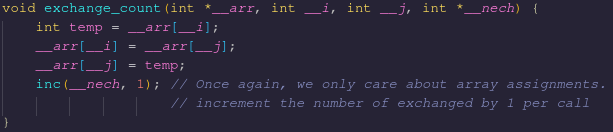
\includegraphics[width=0.5\textwidth]{media/exchange_count.png}
    \caption{Implémentation d'une procédure qui échange deux éléments d'un tableau et qui incrémente une variable (\texttt{*\_\_nech}) qui stocke le nombre d'échanges effectués
    jusqu'au présent.}
\end{figure}


\begin{figure}[h!]
    \centering
    % Created by tikzDevice version 0.12.3.1 on 2022-02-12 23:08:34
% !TEX encoding = UTF-8 Unicode
\begin{tikzpicture}[x=1pt,y=1pt]
\definecolor{fillColor}{RGB}{255,255,255}
\path[use as bounding box,fill=fillColor,fill opacity=0.00] (0,0) rectangle (505.89,216.81);
\begin{scope}
\path[clip] (  0.00,  0.00) rectangle (505.89,216.81);
\definecolor{drawColor}{RGB}{255,255,255}
\definecolor{fillColor}{RGB}{255,255,255}

\path[draw=drawColor,line width= 0.6pt,line join=round,line cap=round,fill=fillColor] (  0.00,  0.00) rectangle (505.89,216.81);
\end{scope}
\begin{scope}
\path[clip] ( 49.31, 30.69) rectangle (422.33,178.94);
\definecolor{fillColor}{gray}{0.92}

\path[fill=fillColor] ( 49.31, 30.69) rectangle (422.33,178.94);
\definecolor{drawColor}{RGB}{255,255,255}

\path[draw=drawColor,line width= 0.3pt,line join=round] ( 49.31, 51.22) --
	(422.33, 51.22);

\path[draw=drawColor,line width= 0.3pt,line join=round] ( 49.31, 78.83) --
	(422.33, 78.83);

\path[draw=drawColor,line width= 0.3pt,line join=round] ( 49.31,106.43) --
	(422.33,106.43);

\path[draw=drawColor,line width= 0.3pt,line join=round] ( 49.31,134.04) --
	(422.33,134.04);

\path[draw=drawColor,line width= 0.3pt,line join=round] ( 49.31,161.65) --
	(422.33,161.65);

\path[draw=drawColor,line width= 0.3pt,line join=round] ( 99.76, 30.69) --
	( 99.76,178.94);

\path[draw=drawColor,line width= 0.3pt,line join=round] (168.13, 30.69) --
	(168.13,178.94);

\path[draw=drawColor,line width= 0.3pt,line join=round] (236.50, 30.69) --
	(236.50,178.94);

\path[draw=drawColor,line width= 0.3pt,line join=round] (304.87, 30.69) --
	(304.87,178.94);

\path[draw=drawColor,line width= 0.3pt,line join=round] (373.24, 30.69) --
	(373.24,178.94);

\path[draw=drawColor,line width= 0.6pt,line join=round] ( 49.31, 37.41) --
	(422.33, 37.41);

\path[draw=drawColor,line width= 0.6pt,line join=round] ( 49.31, 65.02) --
	(422.33, 65.02);

\path[draw=drawColor,line width= 0.6pt,line join=round] ( 49.31, 92.63) --
	(422.33, 92.63);

\path[draw=drawColor,line width= 0.6pt,line join=round] ( 49.31,120.24) --
	(422.33,120.24);

\path[draw=drawColor,line width= 0.6pt,line join=round] ( 49.31,147.85) --
	(422.33,147.85);

\path[draw=drawColor,line width= 0.6pt,line join=round] ( 49.31,175.45) --
	(422.33,175.45);

\path[draw=drawColor,line width= 0.6pt,line join=round] ( 65.58, 30.69) --
	( 65.58,178.94);

\path[draw=drawColor,line width= 0.6pt,line join=round] (133.95, 30.69) --
	(133.95,178.94);

\path[draw=drawColor,line width= 0.6pt,line join=round] (202.32, 30.69) --
	(202.32,178.94);

\path[draw=drawColor,line width= 0.6pt,line join=round] (270.69, 30.69) --
	(270.69,178.94);

\path[draw=drawColor,line width= 0.6pt,line join=round] (339.05, 30.69) --
	(339.05,178.94);

\path[draw=drawColor,line width= 0.6pt,line join=round] (407.42, 30.69) --
	(407.42,178.94);
\definecolor{drawColor}{RGB}{0,0,0}

\path[draw=drawColor,line width= 0.6pt,line join=round] ( 66.26, 37.49) --
	( 69.00, 38.04) --
	( 71.73, 38.70) --
	( 74.47, 39.43) --
	( 77.20, 40.20) --
	( 79.94, 40.99) --
	( 82.67, 41.81) --
	( 85.41, 42.65) --
	( 88.14, 43.51) --
	( 90.88, 44.39) --
	( 93.61, 45.27) --
	( 96.35, 46.17) --
	( 99.08, 47.09) --
	(101.82, 48.01) --
	(104.55, 48.94) --
	(107.28, 49.88) --
	(110.02, 50.83) --
	(112.75, 51.79) --
	(115.49, 52.75) --
	(118.22, 53.72) --
	(120.96, 54.70) --
	(123.69, 55.68) --
	(126.43, 56.67) --
	(129.16, 57.67) --
	(131.90, 58.67) --
	(134.63, 59.68) --
	(137.37, 60.69) --
	(140.10, 61.70) --
	(142.84, 62.73) --
	(145.57, 63.75) --
	(148.31, 64.78) --
	(151.04, 65.82) --
	(153.78, 66.85) --
	(156.51, 67.90) --
	(159.24, 68.94) --
	(161.98, 69.99) --
	(164.71, 71.05) --
	(167.45, 72.10) --
	(170.18, 73.16) --
	(172.92, 74.23) --
	(175.65, 75.29) --
	(178.39, 76.36) --
	(181.12, 77.44) --
	(183.86, 78.51) --
	(186.59, 79.59) --
	(189.33, 80.68) --
	(192.06, 81.76) --
	(194.80, 82.85) --
	(197.53, 83.94) --
	(200.27, 85.03) --
	(203.00, 86.13) --
	(205.74, 87.22) --
	(208.47, 88.33) --
	(211.20, 89.43) --
	(213.94, 90.53) --
	(216.67, 91.64) --
	(219.41, 92.75) --
	(222.14, 93.86) --
	(224.88, 94.98) --
	(227.61, 96.10) --
	(230.35, 97.21) --
	(233.08, 98.34) --
	(235.82, 99.46) --
	(238.55,100.58) --
	(241.29,101.71) --
	(244.02,102.84) --
	(246.76,103.97) --
	(249.49,105.10) --
	(252.23,106.24) --
	(254.96,107.38) --
	(257.70,108.51) --
	(260.43,109.66) --
	(263.17,110.80) --
	(265.90,111.94) --
	(268.63,113.09) --
	(271.37,114.23) --
	(274.10,115.38) --
	(276.84,116.54) --
	(279.57,117.69) --
	(282.31,118.84) --
	(285.04,120.00) --
	(287.78,121.15) --
	(290.51,122.31) --
	(293.25,123.47) --
	(295.98,124.64) --
	(298.72,125.80) --
	(301.45,126.96) --
	(304.19,128.13) --
	(306.92,129.30) --
	(309.66,130.47) --
	(312.39,131.64) --
	(315.13,132.81) --
	(317.86,133.98) --
	(320.59,135.16) --
	(323.33,136.34) --
	(326.06,137.51) --
	(328.80,138.69) --
	(331.53,139.87) --
	(334.27,141.05) --
	(337.00,142.24) --
	(339.74,143.42) --
	(342.47,144.61) --
	(345.21,145.79) --
	(347.94,146.98) --
	(350.68,148.17) --
	(353.41,149.36) --
	(356.15,150.55) --
	(358.88,151.75) --
	(361.62,152.94) --
	(364.35,154.14) --
	(367.09,155.33) --
	(369.82,156.53) --
	(372.55,157.73) --
	(375.29,158.93) --
	(378.02,160.13) --
	(380.76,161.33) --
	(383.49,162.54) --
	(386.23,163.74) --
	(388.96,164.94) --
	(391.70,166.15) --
	(394.43,167.36) --
	(397.17,168.57) --
	(399.90,169.78) --
	(402.64,170.99) --
	(405.37,172.20);
\definecolor{drawColor}{RGB}{0,0,0}

\path[draw=drawColor,draw opacity=0.50,line width= 0.6pt,line join=round] ( 66.26, 37.45) --
	( 69.00, 37.73) --
	( 71.73, 38.06) --
	( 74.47, 38.42) --
	( 77.20, 38.80) --
	( 79.94, 39.20) --
	( 82.67, 39.61) --
	( 85.41, 40.03) --
	( 88.14, 40.46) --
	( 90.88, 40.90) --
	( 93.61, 41.34) --
	( 96.35, 41.79) --
	( 99.08, 42.25) --
	(101.82, 42.71) --
	(104.55, 43.18) --
	(107.28, 43.65) --
	(110.02, 44.12) --
	(112.75, 44.60) --
	(115.49, 45.08) --
	(118.22, 45.57) --
	(120.96, 46.06) --
	(123.69, 46.55) --
	(126.43, 47.04) --
	(129.16, 47.54) --
	(131.90, 48.04) --
	(134.63, 48.55) --
	(137.37, 49.05) --
	(140.10, 49.56) --
	(142.84, 50.07) --
	(145.57, 50.58) --
	(148.31, 51.10) --
	(151.04, 51.61) --
	(153.78, 52.13) --
	(156.51, 52.66) --
	(159.24, 53.18) --
	(161.98, 53.70) --
	(164.71, 54.23) --
	(167.45, 54.76) --
	(170.18, 55.29) --
	(172.92, 55.82) --
	(175.65, 56.35) --
	(178.39, 56.89) --
	(181.12, 57.43) --
	(183.86, 57.96) --
	(186.59, 58.50) --
	(189.33, 59.04) --
	(192.06, 59.59) --
	(194.80, 60.13) --
	(197.53, 60.68) --
	(200.27, 61.22) --
	(203.00, 61.77) --
	(205.74, 62.32) --
	(208.47, 62.87) --
	(211.20, 63.42) --
	(213.94, 63.97) --
	(216.67, 64.53) --
	(219.41, 65.08) --
	(222.14, 65.64) --
	(224.88, 66.20) --
	(227.61, 66.75) --
	(230.35, 67.31) --
	(233.08, 67.87) --
	(235.82, 68.44) --
	(238.55, 69.00) --
	(241.29, 69.56) --
	(244.02, 70.13) --
	(246.76, 70.69) --
	(249.49, 71.26) --
	(252.23, 71.83) --
	(254.96, 72.40) --
	(257.70, 72.96) --
	(260.43, 73.53) --
	(263.17, 74.11) --
	(265.90, 74.68) --
	(268.63, 75.25) --
	(271.37, 75.82) --
	(274.10, 76.40) --
	(276.84, 76.97) --
	(279.57, 77.55) --
	(282.31, 78.13) --
	(285.04, 78.71) --
	(287.78, 79.28) --
	(290.51, 79.86) --
	(293.25, 80.44) --
	(295.98, 81.02) --
	(298.72, 81.61) --
	(301.45, 82.19) --
	(304.19, 82.77) --
	(306.92, 83.36) --
	(309.66, 83.94) --
	(312.39, 84.53) --
	(315.13, 85.11) --
	(317.86, 85.70) --
	(320.59, 86.29) --
	(323.33, 86.87) --
	(326.06, 87.46) --
	(328.80, 88.05) --
	(331.53, 88.64) --
	(334.27, 89.23) --
	(337.00, 89.83) --
	(339.74, 90.42) --
	(342.47, 91.01) --
	(345.21, 91.60) --
	(347.94, 92.20) --
	(350.68, 92.79) --
	(353.41, 93.39) --
	(356.15, 93.98) --
	(358.88, 94.58) --
	(361.62, 95.18) --
	(364.35, 95.78) --
	(367.09, 96.37) --
	(369.82, 96.97) --
	(372.55, 97.57) --
	(375.29, 98.17) --
	(378.02, 98.77) --
	(380.76, 99.37) --
	(383.49, 99.97) --
	(386.23,100.58) --
	(388.96,101.18) --
	(391.70,101.78) --
	(394.43,102.39) --
	(397.17,102.99) --
	(399.90,103.60) --
	(402.64,104.20) --
	(405.37,104.81);
\definecolor{drawColor}{RGB}{248,118,109}

\path[draw=drawColor,line width= 0.6pt,line join=round] ( 66.26, 37.42) --
	( 69.00, 37.53) --
	( 71.73, 37.67) --
	( 74.47, 37.85) --
	( 77.20, 38.04) --
	( 79.94, 38.22) --
	( 82.67, 38.43) --
	( 85.41, 38.62) --
	( 88.14, 38.86) --
	( 90.88, 39.04) --
	( 93.61, 39.27) --
	( 96.35, 39.52) --
	( 99.08, 39.71) --
	(101.82, 39.96) --
	(104.55, 40.16) --
	(107.28, 40.51) --
	(110.02, 40.64) --
	(112.75, 40.95) --
	(115.49, 41.18) --
	(118.22, 41.48) --
	(120.96, 41.64) --
	(123.69, 42.04) --
	(126.43, 42.26) --
	(129.16, 42.49) --
	(131.90, 42.79) --
	(134.63, 42.96) --
	(137.37, 43.28) --
	(140.10, 43.51) --
	(142.84, 43.80) --
	(145.57, 44.09) --
	(148.31, 44.46) --
	(151.04, 44.62) --
	(153.78, 44.97) --
	(156.51, 45.05) --
	(159.24, 45.23) --
	(161.98, 45.73) --
	(164.71, 46.03) --
	(167.45, 46.35) --
	(170.18, 46.55) --
	(172.92, 46.78) --
	(175.65, 47.26) --
	(178.39, 47.35) --
	(181.12, 47.65) --
	(183.86, 47.84) --
	(186.59, 48.47) --
	(189.33, 48.53) --
	(192.06, 48.87) --
	(194.80, 49.44) --
	(197.53, 49.37) --
	(200.27, 49.72) --
	(203.00, 49.87) --
	(205.74, 50.09) --
	(208.47, 50.68) --
	(211.20, 50.85) --
	(213.94, 51.36) --
	(216.67, 51.53) --
	(219.41, 51.94) --
	(222.14, 52.29) --
	(224.88, 52.52) --
	(227.61, 52.50) --
	(230.35, 52.95) --
	(233.08, 53.44) --
	(235.82, 53.77) --
	(238.55, 53.91) --
	(241.29, 54.05) --
	(244.02, 54.55) --
	(246.76, 54.95) --
	(249.49, 55.26) --
	(252.23, 55.40) --
	(254.96, 56.03) --
	(257.70, 56.04) --
	(260.43, 56.35) --
	(263.17, 56.51) --
	(265.90, 57.23) --
	(268.63, 57.20) --
	(271.37, 57.48) --
	(274.10, 57.89) --
	(276.84, 58.20) --
	(279.57, 58.39) --
	(282.31, 58.88) --
	(285.04, 59.34) --
	(287.78, 59.33) --
	(290.51, 59.96) --
	(293.25, 60.20) --
	(295.98, 60.55) --
	(298.72, 60.56) --
	(301.45, 61.03) --
	(304.19, 61.39) --
	(306.92, 61.82) --
	(309.66, 61.84) --
	(312.39, 62.39) --
	(315.13, 62.61) --
	(317.86, 63.06) --
	(320.59, 63.39) --
	(323.33, 63.58) --
	(326.06, 63.59) --
	(328.80, 64.16) --
	(331.53, 64.73) --
	(334.27, 65.25) --
	(337.00, 65.46) --
	(339.74, 65.60) --
	(342.47, 65.90) --
	(345.21, 66.69) --
	(347.94, 66.56) --
	(350.68, 66.83) --
	(353.41, 67.40) --
	(356.15, 67.28) --
	(358.88, 67.98) --
	(361.62, 68.45) --
	(364.35, 68.16) --
	(367.09, 68.68) --
	(369.82, 69.43) --
	(372.55, 69.54) --
	(375.29, 69.51) --
	(378.02, 71.16) --
	(380.76, 70.15) --
	(383.49, 71.29) --
	(386.23, 71.53) --
	(388.96, 71.89) --
	(391.70, 72.45) --
	(394.43, 72.26) --
	(397.17, 72.81) --
	(399.90, 72.85) --
	(402.64, 72.99) --
	(405.37, 73.36);
\definecolor{drawColor}{RGB}{0,0,0}

\path[draw=drawColor,draw opacity=0.25,line width= 0.6pt,line join=round] ( 66.26, 37.43) --
	( 69.00, 37.57) --
	( 71.73, 37.74) --
	( 74.47, 37.92) --
	( 77.20, 38.11) --
	( 79.94, 38.31) --
	( 82.67, 38.51) --
	( 85.41, 38.72) --
	( 88.14, 38.94) --
	( 90.88, 39.16) --
	( 93.61, 39.38) --
	( 96.35, 39.60) --
	( 99.08, 39.83) --
	(101.82, 40.06) --
	(104.55, 40.30) --
	(107.28, 40.53) --
	(110.02, 40.77) --
	(112.75, 41.01) --
	(115.49, 41.25) --
	(118.22, 41.49) --
	(120.96, 41.74) --
	(123.69, 41.98) --
	(126.43, 42.23) --
	(129.16, 42.48) --
	(131.90, 42.73) --
	(134.63, 42.98) --
	(137.37, 43.23) --
	(140.10, 43.49) --
	(142.84, 43.74) --
	(145.57, 44.00) --
	(148.31, 44.26) --
	(151.04, 44.51) --
	(153.78, 44.77) --
	(156.51, 45.03) --
	(159.24, 45.30) --
	(161.98, 45.56) --
	(164.71, 45.82) --
	(167.45, 46.09) --
	(170.18, 46.35) --
	(172.92, 46.62) --
	(175.65, 46.88) --
	(178.39, 47.15) --
	(181.12, 47.42) --
	(183.86, 47.69) --
	(186.59, 47.96) --
	(189.33, 48.23) --
	(192.06, 48.50) --
	(194.80, 48.77) --
	(197.53, 49.04) --
	(200.27, 49.32) --
	(203.00, 49.59) --
	(205.74, 49.87) --
	(208.47, 50.14) --
	(211.20, 50.42) --
	(213.94, 50.69) --
	(216.67, 50.97) --
	(219.41, 51.25) --
	(222.14, 51.53) --
	(224.88, 51.81) --
	(227.61, 52.08) --
	(230.35, 52.36) --
	(233.08, 52.64) --
	(235.82, 52.93) --
	(238.55, 53.21) --
	(241.29, 53.49) --
	(244.02, 53.77) --
	(246.76, 54.05) --
	(249.49, 54.34) --
	(252.23, 54.62) --
	(254.96, 54.90) --
	(257.70, 55.19) --
	(260.43, 55.47) --
	(263.17, 55.76) --
	(265.90, 56.05) --
	(268.63, 56.33) --
	(271.37, 56.62) --
	(274.10, 56.91) --
	(276.84, 57.19) --
	(279.57, 57.48) --
	(282.31, 57.77) --
	(285.04, 58.06) --
	(287.78, 58.35) --
	(290.51, 58.64) --
	(293.25, 58.93) --
	(295.98, 59.22) --
	(298.72, 59.51) --
	(301.45, 59.80) --
	(304.19, 60.09) --
	(306.92, 60.39) --
	(309.66, 60.68) --
	(312.39, 60.97) --
	(315.13, 61.26) --
	(317.86, 61.56) --
	(320.59, 61.85) --
	(323.33, 62.14) --
	(326.06, 62.44) --
	(328.80, 62.73) --
	(331.53, 63.03) --
	(334.27, 63.32) --
	(337.00, 63.62) --
	(339.74, 63.92) --
	(342.47, 64.21) --
	(345.21, 64.51) --
	(347.94, 64.81) --
	(350.68, 65.10) --
	(353.41, 65.40) --
	(356.15, 65.70) --
	(358.88, 66.00) --
	(361.62, 66.30) --
	(364.35, 66.59) --
	(367.09, 66.89) --
	(369.82, 67.19) --
	(372.55, 67.49) --
	(375.29, 67.79) --
	(378.02, 68.09) --
	(380.76, 68.39) --
	(383.49, 68.69) --
	(386.23, 69.00) --
	(388.96, 69.30) --
	(391.70, 69.60) --
	(394.43, 69.90) --
	(397.17, 70.20) --
	(399.90, 70.50) --
	(402.64, 70.81) --
	(405.37, 71.11);
\end{scope}
\begin{scope}
\path[clip] (  0.00,  0.00) rectangle (505.89,216.81);
\definecolor{drawColor}{gray}{0.30}

\node[text=drawColor,anchor=base east,inner sep=0pt, outer sep=0pt, scale=  0.88] at ( 44.36, 34.38) {0};

\node[text=drawColor,anchor=base east,inner sep=0pt, outer sep=0pt, scale=  0.88] at ( 44.36, 61.99) {25000};

\node[text=drawColor,anchor=base east,inner sep=0pt, outer sep=0pt, scale=  0.88] at ( 44.36, 89.60) {50000};

\node[text=drawColor,anchor=base east,inner sep=0pt, outer sep=0pt, scale=  0.88] at ( 44.36,117.21) {75000};

\node[text=drawColor,anchor=base east,inner sep=0pt, outer sep=0pt, scale=  0.88] at ( 44.36,144.82) {100000};

\node[text=drawColor,anchor=base east,inner sep=0pt, outer sep=0pt, scale=  0.88] at ( 44.36,172.42) {125000};
\end{scope}
\begin{scope}
\path[clip] (  0.00,  0.00) rectangle (505.89,216.81);
\definecolor{drawColor}{gray}{0.20}

\path[draw=drawColor,line width= 0.6pt,line join=round] ( 46.56, 37.41) --
	( 49.31, 37.41);

\path[draw=drawColor,line width= 0.6pt,line join=round] ( 46.56, 65.02) --
	( 49.31, 65.02);

\path[draw=drawColor,line width= 0.6pt,line join=round] ( 46.56, 92.63) --
	( 49.31, 92.63);

\path[draw=drawColor,line width= 0.6pt,line join=round] ( 46.56,120.24) --
	( 49.31,120.24);

\path[draw=drawColor,line width= 0.6pt,line join=round] ( 46.56,147.85) --
	( 49.31,147.85);

\path[draw=drawColor,line width= 0.6pt,line join=round] ( 46.56,175.45) --
	( 49.31,175.45);
\end{scope}
\begin{scope}
\path[clip] (  0.00,  0.00) rectangle (505.89,216.81);
\definecolor{drawColor}{gray}{0.20}

\path[draw=drawColor,line width= 0.6pt,line join=round] ( 65.58, 27.94) --
	( 65.58, 30.69);

\path[draw=drawColor,line width= 0.6pt,line join=round] (133.95, 27.94) --
	(133.95, 30.69);

\path[draw=drawColor,line width= 0.6pt,line join=round] (202.32, 27.94) --
	(202.32, 30.69);

\path[draw=drawColor,line width= 0.6pt,line join=round] (270.69, 27.94) --
	(270.69, 30.69);

\path[draw=drawColor,line width= 0.6pt,line join=round] (339.05, 27.94) --
	(339.05, 30.69);

\path[draw=drawColor,line width= 0.6pt,line join=round] (407.42, 27.94) --
	(407.42, 30.69);
\end{scope}
\begin{scope}
\path[clip] (  0.00,  0.00) rectangle (505.89,216.81);
\definecolor{drawColor}{gray}{0.30}

\node[text=drawColor,anchor=base,inner sep=0pt, outer sep=0pt, scale=  0.88] at ( 65.58, 19.68) {0};

\node[text=drawColor,anchor=base,inner sep=0pt, outer sep=0pt, scale=  0.88] at (133.95, 19.68) {1000};

\node[text=drawColor,anchor=base,inner sep=0pt, outer sep=0pt, scale=  0.88] at (202.32, 19.68) {2000};

\node[text=drawColor,anchor=base,inner sep=0pt, outer sep=0pt, scale=  0.88] at (270.69, 19.68) {3000};

\node[text=drawColor,anchor=base,inner sep=0pt, outer sep=0pt, scale=  0.88] at (339.05, 19.68) {4000};

\node[text=drawColor,anchor=base,inner sep=0pt, outer sep=0pt, scale=  0.88] at (407.42, 19.68) {5000};
\end{scope}
\begin{scope}
\path[clip] (  0.00,  0.00) rectangle (505.89,216.81);
\definecolor{drawColor}{RGB}{0,0,0}

\node[text=drawColor,anchor=base,inner sep=0pt, outer sep=0pt, scale=  1.10] at (235.82,  7.64) {$n$};
\end{scope}
\begin{scope}
\path[clip] (  0.00,  0.00) rectangle (505.89,216.81);
\definecolor{fillColor}{RGB}{255,255,255}

\path[fill=fillColor] (433.33, 62.80) rectangle (500.39,146.83);
\end{scope}
\begin{scope}
\path[clip] (  0.00,  0.00) rectangle (505.89,216.81);
\definecolor{drawColor}{RGB}{0,0,0}

\node[text=drawColor,anchor=base west,inner sep=0pt, outer sep=0pt, scale=  1.10] at (438.83,132.68) {$f(n)$};
\end{scope}
\begin{scope}
\path[clip] (  0.00,  0.00) rectangle (505.89,216.81);
\definecolor{fillColor}{gray}{0.95}

\path[fill=fillColor] (438.83,111.66) rectangle (453.28,126.11);
\end{scope}
\begin{scope}
\path[clip] (  0.00,  0.00) rectangle (505.89,216.81);
\definecolor{drawColor}{RGB}{0,0,0}

\path[draw=drawColor,line width= 0.6pt,line join=round] (440.27,118.89) -- (451.84,118.89);
\end{scope}
\begin{scope}
\path[clip] (  0.00,  0.00) rectangle (505.89,216.81);
\definecolor{fillColor}{gray}{0.95}

\path[fill=fillColor] (438.83, 97.20) rectangle (453.28,111.66);
\end{scope}
\begin{scope}
\path[clip] (  0.00,  0.00) rectangle (505.89,216.81);
\definecolor{drawColor}{RGB}{0,0,0}

\path[draw=drawColor,draw opacity=0.50,line width= 0.6pt,line join=round] (440.27,104.43) -- (451.84,104.43);
\end{scope}
\begin{scope}
\path[clip] (  0.00,  0.00) rectangle (505.89,216.81);
\definecolor{fillColor}{gray}{0.95}

\path[fill=fillColor] (438.83, 82.75) rectangle (453.28, 97.20);
\end{scope}
\begin{scope}
\path[clip] (  0.00,  0.00) rectangle (505.89,216.81);
\definecolor{drawColor}{RGB}{248,118,109}

\path[draw=drawColor,line width= 0.6pt,line join=round] (440.27, 89.98) -- (451.84, 89.98);
\end{scope}
\begin{scope}
\path[clip] (  0.00,  0.00) rectangle (505.89,216.81);
\definecolor{fillColor}{gray}{0.95}

\path[fill=fillColor] (438.83, 68.30) rectangle (453.28, 82.75);
\end{scope}
\begin{scope}
\path[clip] (  0.00,  0.00) rectangle (505.89,216.81);
\definecolor{drawColor}{RGB}{0,0,0}

\path[draw=drawColor,draw opacity=0.25,line width= 0.6pt,line join=round] (440.27, 75.52) -- (451.84, 75.52);
\end{scope}
\begin{scope}
\path[clip] (  0.00,  0.00) rectangle (505.89,216.81);
\definecolor{drawColor}{RGB}{0,0,0}

\node[text=drawColor,anchor=base west,inner sep=0pt, outer sep=0pt, scale=  0.88] at (458.78,115.86) {$2n \log n$};
\end{scope}
\begin{scope}
\path[clip] (  0.00,  0.00) rectangle (505.89,216.81);
\definecolor{drawColor}{RGB}{0,0,0}

\node[text=drawColor,anchor=base west,inner sep=0pt, outer sep=0pt, scale=  0.88] at (458.78,101.40) {$n \log n$};
\end{scope}
\begin{scope}
\path[clip] (  0.00,  0.00) rectangle (505.89,216.81);
\definecolor{drawColor}{RGB}{0,0,0}

\node[text=drawColor,anchor=base west,inner sep=0pt, outer sep=0pt, scale=  0.88] at (458.78, 86.95) {$\mu_{ech}$};
\end{scope}
\begin{scope}
\path[clip] (  0.00,  0.00) rectangle (505.89,216.81);
\definecolor{drawColor}{RGB}{0,0,0}

\node[text=drawColor,anchor=base west,inner sep=0pt, outer sep=0pt, scale=  0.88] at (458.78, 72.49) {$0.5n \log n$};
\end{scope}
\begin{scope}
\path[clip] (  0.00,  0.00) rectangle (505.89,216.81);
\definecolor{drawColor}{RGB}{0,0,0}

\node[text=drawColor,anchor=base west,inner sep=0pt, outer sep=0pt, scale=  1.10] at ( 49.31,186.58) {$\texttt{nombreEchanges(n)} \in \Theta(n \log n)$};
\end{scope}
\begin{scope}
\path[clip] (  0.00,  0.00) rectangle (505.89,216.81);
\definecolor{drawColor}{RGB}{0,0,0}

\node[text=drawColor,anchor=base west,inner sep=0pt, outer sep=0pt, scale=  1.32] at ( 49.31,202.22) {Moyenne des échanges};
\end{scope}
\end{tikzpicture}

    \vspace{-1cm}
    \caption{Le moyenne nombre d'échanges se situe entre $n \log n$ et $\frac{1}{2}n \log $. En réalisant une regression linéaire on trouve que
    $\texttt{nombreEchanges}(n) \approx 0.5399(n \log n) - 370.9022$ avec un coefficient de correlation $r = 0.999788$, erreur moyenne carré (MSE) $= 40429.08$, RMS $= 201.0698$.}
\end{figure}

En accord avec nos suivis à la trace de la procédure \texttt{partitionBis}, on remarque qu'il y a, en moyenne, moins d'échanges que de comparaisons au cours du tri. Cela n'est pas étonnant.
On a constaté que la procédure vérifie $(n - 1)$ comparaisons pour \textbf{chaque} appel à \texttt{partitionBis}. Cependant, il se peut qu'on effectue aucun échange pourvu que le tableau donné
en entrée est déjà trié. Ce déséquilibre explique la difference de valeurs de $\alpha$ dans la regression linéaire.
\pagestyle{plain}
Pour procéder, on visualise la complexité des échanges et comparaisons ensemble.

\begin{figure}[h!]
   \centering
   % Created by tikzDevice version 0.12.3.1 on 2022-02-13 15:15:12
% !TEX encoding = UTF-8 Unicode
\begin{tikzpicture}[x=1pt,y=1pt]
\definecolor{fillColor}{RGB}{255,255,255}
\path[use as bounding box,fill=fillColor,fill opacity=0.00] (0,0) rectangle (505.89,216.81);
\begin{scope}
\path[clip] (  0.00,  0.00) rectangle (505.89,216.81);
\definecolor{drawColor}{RGB}{255,255,255}
\definecolor{fillColor}{RGB}{255,255,255}

\path[draw=drawColor,line width= 0.6pt,line join=round,line cap=round,fill=fillColor] (  0.00,  0.00) rectangle (505.89,216.81);
\end{scope}
\begin{scope}
\path[clip] ( 49.31, 30.69) rectangle (412.57,178.94);
\definecolor{fillColor}{gray}{0.92}

\path[fill=fillColor] ( 49.31, 30.69) rectangle (412.57,178.94);
\definecolor{drawColor}{RGB}{255,255,255}

\path[draw=drawColor,line width= 0.3pt,line join=round] ( 49.31, 51.22) --
	(412.57, 51.22);

\path[draw=drawColor,line width= 0.3pt,line join=round] ( 49.31, 78.83) --
	(412.57, 78.83);

\path[draw=drawColor,line width= 0.3pt,line join=round] ( 49.31,106.43) --
	(412.57,106.43);

\path[draw=drawColor,line width= 0.3pt,line join=round] ( 49.31,134.04) --
	(412.57,134.04);

\path[draw=drawColor,line width= 0.3pt,line join=round] ( 49.31,161.65) --
	(412.57,161.65);

\path[draw=drawColor,line width= 0.3pt,line join=round] ( 98.44, 30.69) --
	( 98.44,178.94);

\path[draw=drawColor,line width= 0.3pt,line join=round] (165.03, 30.69) --
	(165.03,178.94);

\path[draw=drawColor,line width= 0.3pt,line join=round] (231.61, 30.69) --
	(231.61,178.94);

\path[draw=drawColor,line width= 0.3pt,line join=round] (298.19, 30.69) --
	(298.19,178.94);

\path[draw=drawColor,line width= 0.3pt,line join=round] (364.77, 30.69) --
	(364.77,178.94);

\path[draw=drawColor,line width= 0.6pt,line join=round] ( 49.31, 37.41) --
	(412.57, 37.41);

\path[draw=drawColor,line width= 0.6pt,line join=round] ( 49.31, 65.02) --
	(412.57, 65.02);

\path[draw=drawColor,line width= 0.6pt,line join=round] ( 49.31, 92.63) --
	(412.57, 92.63);

\path[draw=drawColor,line width= 0.6pt,line join=round] ( 49.31,120.24) --
	(412.57,120.24);

\path[draw=drawColor,line width= 0.6pt,line join=round] ( 49.31,147.85) --
	(412.57,147.85);

\path[draw=drawColor,line width= 0.6pt,line join=round] ( 49.31,175.45) --
	(412.57,175.45);

\path[draw=drawColor,line width= 0.6pt,line join=round] ( 65.15, 30.69) --
	( 65.15,178.94);

\path[draw=drawColor,line width= 0.6pt,line join=round] (131.74, 30.69) --
	(131.74,178.94);

\path[draw=drawColor,line width= 0.6pt,line join=round] (198.32, 30.69) --
	(198.32,178.94);

\path[draw=drawColor,line width= 0.6pt,line join=round] (264.90, 30.69) --
	(264.90,178.94);

\path[draw=drawColor,line width= 0.6pt,line join=round] (331.48, 30.69) --
	(331.48,178.94);

\path[draw=drawColor,line width= 0.6pt,line join=round] (398.06, 30.69) --
	(398.06,178.94);
\definecolor{drawColor}{RGB}{0,0,0}

\path[draw=drawColor,line width= 0.6pt,line join=round] ( 65.82, 37.49) --
	( 68.48, 38.04) --
	( 71.15, 38.70) --
	( 73.81, 39.43) --
	( 76.47, 40.20) --
	( 79.14, 40.99) --
	( 81.80, 41.81) --
	( 84.46, 42.65) --
	( 87.13, 43.51) --
	( 89.79, 44.39) --
	( 92.45, 45.27) --
	( 95.12, 46.17) --
	( 97.78, 47.09) --
	(100.44, 48.01) --
	(103.11, 48.94) --
	(105.77, 49.88) --
	(108.43, 50.83) --
	(111.10, 51.79) --
	(113.76, 52.75) --
	(116.42, 53.72) --
	(119.09, 54.70) --
	(121.75, 55.68) --
	(124.41, 56.67) --
	(127.07, 57.67) --
	(129.74, 58.67) --
	(132.40, 59.68) --
	(135.06, 60.69) --
	(137.73, 61.70) --
	(140.39, 62.73) --
	(143.05, 63.75) --
	(145.72, 64.78) --
	(148.38, 65.82) --
	(151.04, 66.85) --
	(153.71, 67.90) --
	(156.37, 68.94) --
	(159.03, 69.99) --
	(161.70, 71.05) --
	(164.36, 72.10) --
	(167.02, 73.16) --
	(169.69, 74.23) --
	(172.35, 75.29) --
	(175.01, 76.36) --
	(177.68, 77.44) --
	(180.34, 78.51) --
	(183.00, 79.59) --
	(185.67, 80.68) --
	(188.33, 81.76) --
	(190.99, 82.85) --
	(193.66, 83.94) --
	(196.32, 85.03) --
	(198.98, 86.13) --
	(201.65, 87.22) --
	(204.31, 88.33) --
	(206.97, 89.43) --
	(209.64, 90.53) --
	(212.30, 91.64) --
	(214.96, 92.75) --
	(217.63, 93.86) --
	(220.29, 94.98) --
	(222.95, 96.10) --
	(225.61, 97.21) --
	(228.28, 98.34) --
	(230.94, 99.46) --
	(233.60,100.58) --
	(236.27,101.71) --
	(238.93,102.84) --
	(241.59,103.97) --
	(244.26,105.10) --
	(246.92,106.24) --
	(249.58,107.38) --
	(252.25,108.51) --
	(254.91,109.66) --
	(257.57,110.80) --
	(260.24,111.94) --
	(262.90,113.09) --
	(265.56,114.23) --
	(268.23,115.38) --
	(270.89,116.54) --
	(273.55,117.69) --
	(276.22,118.84) --
	(278.88,120.00) --
	(281.54,121.15) --
	(284.21,122.31) --
	(286.87,123.47) --
	(289.53,124.64) --
	(292.20,125.80) --
	(294.86,126.96) --
	(297.52,128.13) --
	(300.19,129.30) --
	(302.85,130.47) --
	(305.51,131.64) --
	(308.18,132.81) --
	(310.84,133.98) --
	(313.50,135.16) --
	(316.17,136.34) --
	(318.83,137.51) --
	(321.49,138.69) --
	(324.15,139.87) --
	(326.82,141.05) --
	(329.48,142.24) --
	(332.14,143.42) --
	(334.81,144.61) --
	(337.47,145.79) --
	(340.13,146.98) --
	(342.80,148.17) --
	(345.46,149.36) --
	(348.12,150.55) --
	(350.79,151.75) --
	(353.45,152.94) --
	(356.11,154.14) --
	(358.78,155.33) --
	(361.44,156.53) --
	(364.10,157.73) --
	(366.77,158.93) --
	(369.43,160.13) --
	(372.09,161.33) --
	(374.76,162.54) --
	(377.42,163.74) --
	(380.08,164.94) --
	(382.75,166.15) --
	(385.41,167.36) --
	(388.07,168.57) --
	(390.74,169.78) --
	(393.40,170.99) --
	(396.06,172.20);
\definecolor{drawColor}{RGB}{199,124,255}

\path[draw=drawColor,line width= 0.6pt,line join=round] ( 65.82, 37.45) --
	( 68.48, 37.81) --
	( 71.15, 38.29) --
	( 73.81, 38.85) --
	( 76.47, 39.44) --
	( 79.14, 40.05) --
	( 81.80, 40.70) --
	( 84.46, 41.39) --
	( 87.13, 42.06) --
	( 89.79, 42.73) --
	( 92.45, 43.43) --
	( 95.12, 44.16) --
	( 97.78, 44.87) --
	(100.44, 45.64) --
	(103.11, 46.34) --
	(105.77, 47.29) --
	(108.43, 47.83) --
	(111.10, 48.79) --
	(113.76, 49.48) --
	(116.42, 50.33) --
	(119.09, 51.12) --
	(121.75, 52.09) --
	(124.41, 52.90) --
	(127.07, 53.76) --
	(129.74, 54.47) --
	(132.40, 55.22) --
	(135.06, 55.97) --
	(137.73, 56.85) --
	(140.39, 57.78) --
	(143.05, 58.66) --
	(145.72, 59.74) --
	(148.38, 60.34) --
	(151.04, 61.31) --
	(153.71, 61.84) --
	(156.37, 62.69) --
	(159.03, 63.79) --
	(161.70, 64.85) --
	(164.36, 65.75) --
	(167.02, 66.53) --
	(169.69, 67.48) --
	(172.35, 68.48) --
	(175.01, 69.17) --
	(177.68, 70.25) --
	(180.34, 70.93) --
	(183.00, 72.14) --
	(185.67, 72.83) --
	(188.33, 73.79) --
	(190.99, 75.17) --
	(193.66, 75.27) --
	(196.32, 76.52) --
	(198.98, 77.35) --
	(201.65, 78.26) --
	(204.31, 79.42) --
	(206.97, 80.20) --
	(209.64, 81.58) --
	(212.30, 82.38) --
	(214.96, 83.16) --
	(217.63, 84.32) --
	(220.29, 84.95) --
	(222.95, 85.63) --
	(225.61, 86.72) --
	(228.28, 88.10) --
	(230.94, 89.19) --
	(233.60, 89.89) --
	(236.27, 90.41) --
	(238.93, 91.81) --
	(241.59, 92.81) --
	(244.26, 93.56) --
	(246.92, 94.75) --
	(249.58, 96.08) --
	(252.25, 96.44) --
	(254.91, 97.45) --
	(257.57, 98.04) --
	(260.24, 99.75) --
	(262.90,100.55) --
	(265.56,101.09) --
	(268.23,102.59) --
	(270.89,103.12) --
	(273.55,104.27) --
	(276.22,105.19) --
	(278.88,106.47) --
	(281.54,106.93) --
	(284.21,108.53) --
	(286.87,109.41) --
	(289.53,110.84) --
	(292.20,111.31) --
	(294.86,112.11) --
	(297.52,113.97) --
	(300.19,114.31) --
	(302.85,115.14) --
	(305.51,116.32) --
	(308.18,116.69) --
	(310.84,118.56) --
	(313.50,119.53) --
	(316.17,119.89) --
	(318.83,121.00) --
	(321.49,122.33) --
	(324.15,123.59) --
	(326.82,124.86) --
	(329.48,125.43) --
	(332.14,126.54) --
	(334.81,127.84) --
	(337.47,129.01) --
	(340.13,129.65) --
	(342.80,130.93) --
	(345.46,132.09) --
	(348.12,131.66) --
	(350.79,133.67) --
	(353.45,134.77) --
	(356.11,134.84) --
	(358.78,136.53) --
	(361.44,138.51) --
	(364.10,138.47) --
	(366.77,139.34) --
	(369.43,142.79) --
	(372.09,141.33) --
	(374.76,143.67) --
	(377.42,144.32) --
	(380.08,146.07) --
	(382.75,147.16) --
	(385.41,146.97) --
	(388.07,148.43) --
	(390.74,149.12) --
	(393.40,149.89) --
	(396.06,151.26);
\definecolor{drawColor}{RGB}{248,118,109}

\path[draw=drawColor,line width= 0.6pt,line join=round] ( 65.82, 37.44) --
	( 68.48, 37.70) --
	( 71.15, 38.03) --
	( 73.81, 38.41) --
	( 76.47, 38.82) --
	( 79.14, 39.24) --
	( 81.80, 39.69) --
	( 84.46, 40.18) --
	( 87.13, 40.62) --
	( 89.79, 41.11) --
	( 92.45, 41.57) --
	( 95.12, 42.06) --
	( 97.78, 42.57) --
	(100.44, 43.10) --
	(103.11, 43.59) --
	(105.77, 44.19) --
	(108.43, 44.60) --
	(111.10, 45.25) --
	(113.76, 45.71) --
	(116.42, 46.27) --
	(119.09, 46.89) --
	(121.75, 47.47) --
	(124.41, 48.05) --
	(127.07, 48.69) --
	(129.74, 49.10) --
	(132.40, 49.67) --
	(135.06, 50.10) --
	(137.73, 50.75) --
	(140.39, 51.39) --
	(143.05, 51.99) --
	(145.72, 52.69) --
	(148.38, 53.13) --
	(151.04, 53.75) --
	(153.71, 54.20) --
	(156.37, 54.87) --
	(159.03, 55.47) --
	(161.70, 56.24) --
	(164.36, 56.82) --
	(167.02, 57.39) --
	(169.69, 58.11) --
	(172.35, 58.64) --
	(175.01, 59.23) --
	(177.68, 60.01) --
	(180.34, 60.51) --
	(183.00, 61.08) --
	(185.67, 61.71) --
	(188.33, 62.33) --
	(190.99, 63.14) --
	(193.66, 63.32) --
	(196.32, 64.21) --
	(198.98, 64.89) --
	(201.65, 65.58) --
	(204.31, 66.15) --
	(206.97, 66.76) --
	(209.64, 67.64) --
	(212.30, 68.26) --
	(214.96, 68.63) --
	(217.63, 69.44) --
	(220.29, 69.85) --
	(222.95, 70.54) --
	(225.61, 71.18) --
	(228.28, 72.07) --
	(230.94, 72.84) --
	(233.60, 73.39) --
	(236.27, 73.78) --
	(238.93, 74.67) --
	(241.59, 75.27) --
	(244.26, 75.71) --
	(246.92, 76.77) --
	(249.58, 77.47) --
	(252.25, 77.81) --
	(254.91, 78.51) --
	(257.57, 78.95) --
	(260.24, 79.94) --
	(262.90, 80.76) --
	(265.56, 81.02) --
	(268.23, 82.11) --
	(270.89, 82.33) --
	(273.55, 83.30) --
	(276.22, 83.73) --
	(278.88, 84.55) --
	(281.54, 85.01) --
	(284.21, 85.98) --
	(286.87, 86.62) --
	(289.53, 87.70) --
	(292.20, 88.17) --
	(294.86, 88.49) --
	(297.52, 89.99) --
	(300.19, 89.91) --
	(302.85, 90.72) --
	(305.51, 91.34) --
	(308.18, 91.50) --
	(310.84, 92.92) --
	(313.50, 93.55) --
	(316.17, 93.72) --
	(318.83, 94.82) --
	(321.49, 95.58) --
	(324.15, 96.28) --
	(326.82, 97.03) --
	(329.48, 97.39) --
	(332.14, 98.36) --
	(334.81, 99.35) --
	(337.47, 99.73) --
	(340.13,100.51) --
	(342.80,101.52) --
	(345.46,102.11) --
	(348.12,101.79) --
	(350.79,103.10) --
	(353.45,103.73) --
	(356.11,104.09) --
	(358.78,105.26) --
	(361.44,106.49) --
	(364.10,106.34) --
	(366.77,107.24) --
	(369.43,109.04) --
	(372.09,108.59) --
	(374.76,109.80) --
	(377.42,110.20) --
	(380.08,111.59) --
	(382.75,112.13) --
	(385.41,112.12) --
	(388.07,113.04) --
	(390.74,113.68) --
	(393.40,114.32) --
	(396.06,115.31);
\definecolor{drawColor}{RGB}{0,191,196}

\path[draw=drawColor,line width= 0.6pt,line join=round] ( 65.82, 37.42) --
	( 68.48, 37.53) --
	( 71.15, 37.67) --
	( 73.81, 37.85) --
	( 76.47, 38.04) --
	( 79.14, 38.22) --
	( 81.80, 38.43) --
	( 84.46, 38.62) --
	( 87.13, 38.86) --
	( 89.79, 39.04) --
	( 92.45, 39.27) --
	( 95.12, 39.52) --
	( 97.78, 39.71) --
	(100.44, 39.96) --
	(103.11, 40.16) --
	(105.77, 40.51) --
	(108.43, 40.64) --
	(111.10, 40.95) --
	(113.76, 41.18) --
	(116.42, 41.48) --
	(119.09, 41.64) --
	(121.75, 42.04) --
	(124.41, 42.26) --
	(127.07, 42.49) --
	(129.74, 42.79) --
	(132.40, 42.96) --
	(135.06, 43.28) --
	(137.73, 43.51) --
	(140.39, 43.80) --
	(143.05, 44.09) --
	(145.72, 44.46) --
	(148.38, 44.62) --
	(151.04, 44.97) --
	(153.71, 45.05) --
	(156.37, 45.23) --
	(159.03, 45.73) --
	(161.70, 46.03) --
	(164.36, 46.35) --
	(167.02, 46.55) --
	(169.69, 46.78) --
	(172.35, 47.26) --
	(175.01, 47.35) --
	(177.68, 47.65) --
	(180.34, 47.84) --
	(183.00, 48.47) --
	(185.67, 48.53) --
	(188.33, 48.87) --
	(190.99, 49.44) --
	(193.66, 49.37) --
	(196.32, 49.72) --
	(198.98, 49.87) --
	(201.65, 50.09) --
	(204.31, 50.68) --
	(206.97, 50.85) --
	(209.64, 51.36) --
	(212.30, 51.53) --
	(214.96, 51.94) --
	(217.63, 52.29) --
	(220.29, 52.52) --
	(222.95, 52.50) --
	(225.61, 52.95) --
	(228.28, 53.44) --
	(230.94, 53.77) --
	(233.60, 53.91) --
	(236.27, 54.05) --
	(238.93, 54.55) --
	(241.59, 54.95) --
	(244.26, 55.26) --
	(246.92, 55.40) --
	(249.58, 56.03) --
	(252.25, 56.04) --
	(254.91, 56.35) --
	(257.57, 56.51) --
	(260.24, 57.23) --
	(262.90, 57.20) --
	(265.56, 57.48) --
	(268.23, 57.89) --
	(270.89, 58.20) --
	(273.55, 58.39) --
	(276.22, 58.88) --
	(278.88, 59.34) --
	(281.54, 59.33) --
	(284.21, 59.96) --
	(286.87, 60.20) --
	(289.53, 60.55) --
	(292.20, 60.56) --
	(294.86, 61.03) --
	(297.52, 61.39) --
	(300.19, 61.82) --
	(302.85, 61.84) --
	(305.51, 62.39) --
	(308.18, 62.61) --
	(310.84, 63.06) --
	(313.50, 63.39) --
	(316.17, 63.58) --
	(318.83, 63.59) --
	(321.49, 64.16) --
	(324.15, 64.73) --
	(326.82, 65.25) --
	(329.48, 65.46) --
	(332.14, 65.60) --
	(334.81, 65.90) --
	(337.47, 66.69) --
	(340.13, 66.56) --
	(342.80, 66.83) --
	(345.46, 67.40) --
	(348.12, 67.28) --
	(350.79, 67.98) --
	(353.45, 68.45) --
	(356.11, 68.16) --
	(358.78, 68.68) --
	(361.44, 69.43) --
	(364.10, 69.54) --
	(366.77, 69.51) --
	(369.43, 71.16) --
	(372.09, 70.15) --
	(374.76, 71.29) --
	(377.42, 71.53) --
	(380.08, 71.89) --
	(382.75, 72.45) --
	(385.41, 72.26) --
	(388.07, 72.81) --
	(390.74, 72.85) --
	(393.40, 72.99) --
	(396.06, 73.36);
\definecolor{drawColor}{RGB}{0,0,0}

\path[draw=drawColor,draw opacity=0.25,line width= 0.6pt,line join=round] ( 65.82, 37.43) --
	( 68.48, 37.57) --
	( 71.15, 37.74) --
	( 73.81, 37.92) --
	( 76.47, 38.11) --
	( 79.14, 38.31) --
	( 81.80, 38.51) --
	( 84.46, 38.72) --
	( 87.13, 38.94) --
	( 89.79, 39.16) --
	( 92.45, 39.38) --
	( 95.12, 39.60) --
	( 97.78, 39.83) --
	(100.44, 40.06) --
	(103.11, 40.30) --
	(105.77, 40.53) --
	(108.43, 40.77) --
	(111.10, 41.01) --
	(113.76, 41.25) --
	(116.42, 41.49) --
	(119.09, 41.74) --
	(121.75, 41.98) --
	(124.41, 42.23) --
	(127.07, 42.48) --
	(129.74, 42.73) --
	(132.40, 42.98) --
	(135.06, 43.23) --
	(137.73, 43.49) --
	(140.39, 43.74) --
	(143.05, 44.00) --
	(145.72, 44.26) --
	(148.38, 44.51) --
	(151.04, 44.77) --
	(153.71, 45.03) --
	(156.37, 45.30) --
	(159.03, 45.56) --
	(161.70, 45.82) --
	(164.36, 46.09) --
	(167.02, 46.35) --
	(169.69, 46.62) --
	(172.35, 46.88) --
	(175.01, 47.15) --
	(177.68, 47.42) --
	(180.34, 47.69) --
	(183.00, 47.96) --
	(185.67, 48.23) --
	(188.33, 48.50) --
	(190.99, 48.77) --
	(193.66, 49.04) --
	(196.32, 49.32) --
	(198.98, 49.59) --
	(201.65, 49.87) --
	(204.31, 50.14) --
	(206.97, 50.42) --
	(209.64, 50.69) --
	(212.30, 50.97) --
	(214.96, 51.25) --
	(217.63, 51.53) --
	(220.29, 51.81) --
	(222.95, 52.08) --
	(225.61, 52.36) --
	(228.28, 52.64) --
	(230.94, 52.93) --
	(233.60, 53.21) --
	(236.27, 53.49) --
	(238.93, 53.77) --
	(241.59, 54.05) --
	(244.26, 54.34) --
	(246.92, 54.62) --
	(249.58, 54.90) --
	(252.25, 55.19) --
	(254.91, 55.47) --
	(257.57, 55.76) --
	(260.24, 56.05) --
	(262.90, 56.33) --
	(265.56, 56.62) --
	(268.23, 56.91) --
	(270.89, 57.19) --
	(273.55, 57.48) --
	(276.22, 57.77) --
	(278.88, 58.06) --
	(281.54, 58.35) --
	(284.21, 58.64) --
	(286.87, 58.93) --
	(289.53, 59.22) --
	(292.20, 59.51) --
	(294.86, 59.80) --
	(297.52, 60.09) --
	(300.19, 60.39) --
	(302.85, 60.68) --
	(305.51, 60.97) --
	(308.18, 61.26) --
	(310.84, 61.56) --
	(313.50, 61.85) --
	(316.17, 62.14) --
	(318.83, 62.44) --
	(321.49, 62.73) --
	(324.15, 63.03) --
	(326.82, 63.32) --
	(329.48, 63.62) --
	(332.14, 63.92) --
	(334.81, 64.21) --
	(337.47, 64.51) --
	(340.13, 64.81) --
	(342.80, 65.10) --
	(345.46, 65.40) --
	(348.12, 65.70) --
	(350.79, 66.00) --
	(353.45, 66.30) --
	(356.11, 66.59) --
	(358.78, 66.89) --
	(361.44, 67.19) --
	(364.10, 67.49) --
	(366.77, 67.79) --
	(369.43, 68.09) --
	(372.09, 68.39) --
	(374.76, 68.69) --
	(377.42, 69.00) --
	(380.08, 69.30) --
	(382.75, 69.60) --
	(385.41, 69.90) --
	(388.07, 70.20) --
	(390.74, 70.50) --
	(393.40, 70.81) --
	(396.06, 71.11);
\end{scope}
\begin{scope}
\path[clip] (  0.00,  0.00) rectangle (505.89,216.81);
\definecolor{drawColor}{gray}{0.30}

\node[text=drawColor,anchor=base east,inner sep=0pt, outer sep=0pt, scale=  0.88] at ( 44.36, 34.38) {0};

\node[text=drawColor,anchor=base east,inner sep=0pt, outer sep=0pt, scale=  0.88] at ( 44.36, 61.99) {25000};

\node[text=drawColor,anchor=base east,inner sep=0pt, outer sep=0pt, scale=  0.88] at ( 44.36, 89.60) {50000};

\node[text=drawColor,anchor=base east,inner sep=0pt, outer sep=0pt, scale=  0.88] at ( 44.36,117.21) {75000};

\node[text=drawColor,anchor=base east,inner sep=0pt, outer sep=0pt, scale=  0.88] at ( 44.36,144.82) {100000};

\node[text=drawColor,anchor=base east,inner sep=0pt, outer sep=0pt, scale=  0.88] at ( 44.36,172.42) {125000};
\end{scope}
\begin{scope}
\path[clip] (  0.00,  0.00) rectangle (505.89,216.81);
\definecolor{drawColor}{gray}{0.20}

\path[draw=drawColor,line width= 0.6pt,line join=round] ( 46.56, 37.41) --
	( 49.31, 37.41);

\path[draw=drawColor,line width= 0.6pt,line join=round] ( 46.56, 65.02) --
	( 49.31, 65.02);

\path[draw=drawColor,line width= 0.6pt,line join=round] ( 46.56, 92.63) --
	( 49.31, 92.63);

\path[draw=drawColor,line width= 0.6pt,line join=round] ( 46.56,120.24) --
	( 49.31,120.24);

\path[draw=drawColor,line width= 0.6pt,line join=round] ( 46.56,147.85) --
	( 49.31,147.85);

\path[draw=drawColor,line width= 0.6pt,line join=round] ( 46.56,175.45) --
	( 49.31,175.45);
\end{scope}
\begin{scope}
\path[clip] (  0.00,  0.00) rectangle (505.89,216.81);
\definecolor{drawColor}{gray}{0.20}

\path[draw=drawColor,line width= 0.6pt,line join=round] ( 65.15, 27.94) --
	( 65.15, 30.69);

\path[draw=drawColor,line width= 0.6pt,line join=round] (131.74, 27.94) --
	(131.74, 30.69);

\path[draw=drawColor,line width= 0.6pt,line join=round] (198.32, 27.94) --
	(198.32, 30.69);

\path[draw=drawColor,line width= 0.6pt,line join=round] (264.90, 27.94) --
	(264.90, 30.69);

\path[draw=drawColor,line width= 0.6pt,line join=round] (331.48, 27.94) --
	(331.48, 30.69);

\path[draw=drawColor,line width= 0.6pt,line join=round] (398.06, 27.94) --
	(398.06, 30.69);
\end{scope}
\begin{scope}
\path[clip] (  0.00,  0.00) rectangle (505.89,216.81);
\definecolor{drawColor}{gray}{0.30}

\node[text=drawColor,anchor=base,inner sep=0pt, outer sep=0pt, scale=  0.88] at ( 65.15, 19.68) {0};

\node[text=drawColor,anchor=base,inner sep=0pt, outer sep=0pt, scale=  0.88] at (131.74, 19.68) {1000};

\node[text=drawColor,anchor=base,inner sep=0pt, outer sep=0pt, scale=  0.88] at (198.32, 19.68) {2000};

\node[text=drawColor,anchor=base,inner sep=0pt, outer sep=0pt, scale=  0.88] at (264.90, 19.68) {3000};

\node[text=drawColor,anchor=base,inner sep=0pt, outer sep=0pt, scale=  0.88] at (331.48, 19.68) {4000};

\node[text=drawColor,anchor=base,inner sep=0pt, outer sep=0pt, scale=  0.88] at (398.06, 19.68) {5000};
\end{scope}
\begin{scope}
\path[clip] (  0.00,  0.00) rectangle (505.89,216.81);
\definecolor{drawColor}{RGB}{0,0,0}

\node[text=drawColor,anchor=base,inner sep=0pt, outer sep=0pt, scale=  1.10] at (230.94,  7.64) {$n$};
\end{scope}
\begin{scope}
\path[clip] (  0.00,  0.00) rectangle (505.89,216.81);
\definecolor{fillColor}{RGB}{255,255,255}

\path[fill=fillColor] (423.57, 55.57) rectangle (500.39,154.05);
\end{scope}
\begin{scope}
\path[clip] (  0.00,  0.00) rectangle (505.89,216.81);
\definecolor{drawColor}{RGB}{0,0,0}

\node[text=drawColor,anchor=base west,inner sep=0pt, outer sep=0pt, scale=  1.10] at (429.07,139.91) {$f(n)$};
\end{scope}
\begin{scope}
\path[clip] (  0.00,  0.00) rectangle (505.89,216.81);
\definecolor{fillColor}{gray}{0.95}

\path[fill=fillColor] (429.07,118.89) rectangle (443.53,133.34);
\end{scope}
\begin{scope}
\path[clip] (  0.00,  0.00) rectangle (505.89,216.81);
\definecolor{drawColor}{RGB}{0,0,0}

\path[draw=drawColor,line width= 0.6pt,line join=round] (430.52,126.11) -- (442.08,126.11);
\end{scope}
\begin{scope}
\path[clip] (  0.00,  0.00) rectangle (505.89,216.81);
\definecolor{fillColor}{gray}{0.95}

\path[fill=fillColor] (429.07,104.43) rectangle (443.53,118.89);
\end{scope}
\begin{scope}
\path[clip] (  0.00,  0.00) rectangle (505.89,216.81);
\definecolor{drawColor}{RGB}{199,124,255}

\path[draw=drawColor,line width= 0.6pt,line join=round] (430.52,111.66) -- (442.08,111.66);
\end{scope}
\begin{scope}
\path[clip] (  0.00,  0.00) rectangle (505.89,216.81);
\definecolor{fillColor}{gray}{0.95}

\path[fill=fillColor] (429.07, 89.98) rectangle (443.53,104.43);
\end{scope}
\begin{scope}
\path[clip] (  0.00,  0.00) rectangle (505.89,216.81);
\definecolor{drawColor}{RGB}{248,118,109}

\path[draw=drawColor,line width= 0.6pt,line join=round] (430.52, 97.20) -- (442.08, 97.20);
\end{scope}
\begin{scope}
\path[clip] (  0.00,  0.00) rectangle (505.89,216.81);
\definecolor{fillColor}{gray}{0.95}

\path[fill=fillColor] (429.07, 75.52) rectangle (443.53, 89.98);
\end{scope}
\begin{scope}
\path[clip] (  0.00,  0.00) rectangle (505.89,216.81);
\definecolor{drawColor}{RGB}{0,191,196}

\path[draw=drawColor,line width= 0.6pt,line join=round] (430.52, 82.75) -- (442.08, 82.75);
\end{scope}
\begin{scope}
\path[clip] (  0.00,  0.00) rectangle (505.89,216.81);
\definecolor{fillColor}{gray}{0.95}

\path[fill=fillColor] (429.07, 61.07) rectangle (443.53, 75.52);
\end{scope}
\begin{scope}
\path[clip] (  0.00,  0.00) rectangle (505.89,216.81);
\definecolor{drawColor}{RGB}{0,0,0}

\path[draw=drawColor,draw opacity=0.25,line width= 0.6pt,line join=round] (430.52, 68.30) -- (442.08, 68.30);
\end{scope}
\begin{scope}
\path[clip] (  0.00,  0.00) rectangle (505.89,216.81);
\definecolor{drawColor}{RGB}{0,0,0}

\node[text=drawColor,anchor=base west,inner sep=0pt, outer sep=0pt, scale=  0.88] at (449.03,123.08) {$2n \log n$};
\end{scope}
\begin{scope}
\path[clip] (  0.00,  0.00) rectangle (505.89,216.81);
\definecolor{drawColor}{RGB}{0,0,0}

\node[text=drawColor,anchor=base west,inner sep=0pt, outer sep=0pt, scale=  0.88] at (449.03,108.63) {$\mu_{cmp} + \mu_{ech}$};
\end{scope}
\begin{scope}
\path[clip] (  0.00,  0.00) rectangle (505.89,216.81);
\definecolor{drawColor}{RGB}{0,0,0}

\node[text=drawColor,anchor=base west,inner sep=0pt, outer sep=0pt, scale=  0.88] at (449.03, 94.17) {$\mu_{cmp}$};
\end{scope}
\begin{scope}
\path[clip] (  0.00,  0.00) rectangle (505.89,216.81);
\definecolor{drawColor}{RGB}{0,0,0}

\node[text=drawColor,anchor=base west,inner sep=0pt, outer sep=0pt, scale=  0.88] at (449.03, 79.72) {$\mu_{ech}$};
\end{scope}
\begin{scope}
\path[clip] (  0.00,  0.00) rectangle (505.89,216.81);
\definecolor{drawColor}{RGB}{0,0,0}

\node[text=drawColor,anchor=base west,inner sep=0pt, outer sep=0pt, scale=  0.88] at (449.03, 65.27) {$0.5n \log n$};
\end{scope}
\begin{scope}
\path[clip] (  0.00,  0.00) rectangle (505.89,216.81);
\definecolor{drawColor}{RGB}{0,0,0}

\node[text=drawColor,anchor=base west,inner sep=0pt, outer sep=0pt, scale=  1.10] at ( 49.31,186.58) {$\texttt{nombresCmpPlusEch}(n) \in \Theta(n \log n)$};
\end{scope}
\begin{scope}
\path[clip] (  0.00,  0.00) rectangle (505.89,216.81);
\definecolor{drawColor}{RGB}{0,0,0}

\node[text=drawColor,anchor=base west,inner sep=0pt, outer sep=0pt, scale=  1.32] at ( 49.31,202.22) {Moyenne des comparaisons et échanges};
\end{scope}
\end{tikzpicture}

   \vspace{-1cm}
   \caption{Une regression linéaire revèle que $\texttt{nombresCmpPlusEch}(n)$ a une valeur de $\alpha_{sum} = 1.7$,  $\texttt{nombresComparaisons}(n)$ a $\alpha_{cmp} = 1.16$,
   et $\texttt{nombresEchanges}(n)$ a $\alpha_{ech} = 0.54$.}
\end{figure}

Toujours bornés par $2 n \log n$, on trouve que la valeur de alpha pour la moyenne du somme des comparaisons et échanges est en effet
le somme des pentes de moyenne comparaisons et de moyenne échanges. Autrement dit, $1.7 = 1.16 + 0.54$.

\begin{itemize}
    \item[5.] D'après votre expérimentation, laquelle des deux méthodes \texttt{partition} et \texttt{partitionBis} est la
    plus efficace?
\end{itemize}

On peut conclure que la méthode \texttt{partition} est la plus efficace, parce que elle fait moins d'échanges que la méthode
\texttt{partitionBis}. Considèrez le graphe suivant.

% \newpage

\begin{figure}[h!]
    \centering
    % Created by tikzDevice version 0.12.3.1 on 2022-02-19 21:06:14
% !TEX encoding = UTF-8 Unicode
\begin{tikzpicture}[x=1pt,y=1pt]
\definecolor{fillColor}{RGB}{255,255,255}
\path[use as bounding box,fill=fillColor,fill opacity=0.00] (0,0) rectangle (505.89,216.81);
\begin{scope}
\path[clip] (  0.00,  0.00) rectangle (505.89,216.81);
\definecolor{drawColor}{RGB}{255,255,255}
\definecolor{fillColor}{RGB}{255,255,255}

\path[draw=drawColor,line width= 0.6pt,line join=round,line cap=round,fill=fillColor] (  0.00,  0.00) rectangle (505.89,216.81);
\end{scope}
\begin{scope}
\path[clip] ( 49.31, 30.69) rectangle (228.19,162.37);
\definecolor{fillColor}{gray}{0.92}

\path[fill=fillColor] ( 49.31, 30.69) rectangle (228.19,162.37);
\definecolor{drawColor}{RGB}{255,255,255}

\path[draw=drawColor,line width= 0.3pt,line join=round] ( 49.31, 48.93) --
	(228.19, 48.93);

\path[draw=drawColor,line width= 0.3pt,line join=round] ( 49.31, 73.45) --
	(228.19, 73.45);

\path[draw=drawColor,line width= 0.3pt,line join=round] ( 49.31, 97.97) --
	(228.19, 97.97);

\path[draw=drawColor,line width= 0.3pt,line join=round] ( 49.31,122.49) --
	(228.19,122.49);

\path[draw=drawColor,line width= 0.3pt,line join=round] ( 49.31,147.01) --
	(228.19,147.01);

\path[draw=drawColor,line width= 0.3pt,line join=round] ( 73.50, 30.69) --
	( 73.50,162.37);

\path[draw=drawColor,line width= 0.3pt,line join=round] (106.29, 30.69) --
	(106.29,162.37);

\path[draw=drawColor,line width= 0.3pt,line join=round] (139.08, 30.69) --
	(139.08,162.37);

\path[draw=drawColor,line width= 0.3pt,line join=round] (171.86, 30.69) --
	(171.86,162.37);

\path[draw=drawColor,line width= 0.3pt,line join=round] (204.65, 30.69) --
	(204.65,162.37);

\path[draw=drawColor,line width= 0.6pt,line join=round] ( 49.31, 36.67) --
	(228.19, 36.67);

\path[draw=drawColor,line width= 0.6pt,line join=round] ( 49.31, 61.19) --
	(228.19, 61.19);

\path[draw=drawColor,line width= 0.6pt,line join=round] ( 49.31, 85.71) --
	(228.19, 85.71);

\path[draw=drawColor,line width= 0.6pt,line join=round] ( 49.31,110.23) --
	(228.19,110.23);

\path[draw=drawColor,line width= 0.6pt,line join=round] ( 49.31,134.75) --
	(228.19,134.75);

\path[draw=drawColor,line width= 0.6pt,line join=round] ( 49.31,159.27) --
	(228.19,159.27);

\path[draw=drawColor,line width= 0.6pt,line join=round] ( 57.11, 30.69) --
	( 57.11,162.37);

\path[draw=drawColor,line width= 0.6pt,line join=round] ( 89.90, 30.69) --
	( 89.90,162.37);

\path[draw=drawColor,line width= 0.6pt,line join=round] (122.68, 30.69) --
	(122.68,162.37);

\path[draw=drawColor,line width= 0.6pt,line join=round] (155.47, 30.69) --
	(155.47,162.37);

\path[draw=drawColor,line width= 0.6pt,line join=round] (188.26, 30.69) --
	(188.26,162.37);

\path[draw=drawColor,line width= 0.6pt,line join=round] (221.04, 30.69) --
	(221.04,162.37);
\definecolor{drawColor}{RGB}{0,0,0}

\path[draw=drawColor,line width= 0.6pt,line join=round] ( 57.44, 36.73) --
	( 58.75, 37.22) --
	( 60.06, 37.81) --
	( 61.37, 38.46) --
	( 62.68, 39.14) --
	( 64.00, 39.85) --
	( 65.31, 40.57) --
	( 66.62, 41.32) --
	( 67.93, 42.08) --
	( 69.24, 42.86) --
	( 70.55, 43.65) --
	( 71.87, 44.45) --
	( 73.18, 45.26) --
	( 74.49, 46.08) --
	( 75.80, 46.90) --
	( 77.11, 47.74) --
	( 78.42, 48.58) --
	( 79.73, 49.43) --
	( 81.05, 50.29) --
	( 82.36, 51.15) --
	( 83.67, 52.02) --
	( 84.98, 52.89) --
	( 86.29, 53.77) --
	( 87.60, 54.66) --
	( 88.91, 55.55) --
	( 90.23, 56.44) --
	( 91.54, 57.34) --
	( 92.85, 58.24) --
	( 94.16, 59.15) --
	( 95.47, 60.06) --
	( 96.78, 60.98) --
	( 98.09, 61.89) --
	( 99.41, 62.82) --
	(100.72, 63.74) --
	(102.03, 64.67) --
	(103.34, 65.60) --
	(104.65, 66.54) --
	(105.96, 67.48) --
	(107.27, 68.42) --
	(108.59, 69.36) --
	(109.90, 70.31) --
	(111.21, 71.26) --
	(112.52, 72.22) --
	(113.83, 73.17) --
	(115.14, 74.13) --
	(116.45, 75.09) --
	(117.77, 76.06) --
	(119.08, 77.02) --
	(120.39, 77.99) --
	(121.70, 78.96) --
	(123.01, 79.93) --
	(124.32, 80.91) --
	(125.64, 81.89) --
	(126.95, 82.87) --
	(128.26, 83.85) --
	(129.57, 84.83) --
	(130.88, 85.82) --
	(132.19, 86.81) --
	(133.50, 87.80) --
	(134.82, 88.79) --
	(136.13, 89.78) --
	(137.44, 90.78) --
	(138.75, 91.77) --
	(140.06, 92.77) --
	(141.37, 93.78) --
	(142.68, 94.78) --
	(144.00, 95.78) --
	(145.31, 96.79) --
	(146.62, 97.80) --
	(147.93, 98.81) --
	(149.24, 99.82) --
	(150.55,100.83) --
	(151.86,101.85) --
	(153.18,102.86) --
	(154.49,103.88) --
	(155.80,104.90) --
	(157.11,105.92) --
	(158.42,106.94) --
	(159.73,107.97) --
	(161.04,108.99) --
	(162.36,110.02) --
	(163.67,111.04) --
	(164.98,112.07) --
	(166.29,113.10) --
	(167.60,114.14) --
	(168.91,115.17) --
	(170.22,116.20) --
	(171.54,117.24) --
	(172.85,118.28) --
	(174.16,119.32) --
	(175.47,120.36) --
	(176.78,121.40) --
	(178.09,122.44) --
	(179.40,123.48) --
	(180.72,124.53) --
	(182.03,125.57) --
	(183.34,126.62) --
	(184.65,127.67) --
	(185.96,128.72) --
	(187.27,129.77) --
	(188.59,130.82) --
	(189.90,131.87) --
	(191.21,132.93) --
	(192.52,133.98) --
	(193.83,135.04) --
	(195.14,136.10) --
	(196.45,137.16) --
	(197.77,138.22) --
	(199.08,139.28) --
	(200.39,140.34) --
	(201.70,141.40) --
	(203.01,142.46) --
	(204.32,143.53) --
	(205.63,144.59) --
	(206.95,145.66) --
	(208.26,146.73) --
	(209.57,147.80) --
	(210.88,148.87) --
	(212.19,149.94) --
	(213.50,151.01) --
	(214.81,152.08) --
	(216.13,153.16) --
	(217.44,154.23) --
	(218.75,155.31) --
	(220.06,156.38);
\definecolor{drawColor}{RGB}{199,124,255}

\path[draw=drawColor,line width= 0.6pt,line join=round] ( 57.44, 36.70) --
	( 58.75, 36.98) --
	( 60.06, 37.33) --
	( 61.37, 37.74) --
	( 62.68, 38.18) --
	( 64.00, 38.62) --
	( 65.31, 39.11) --
	( 66.62, 39.61) --
	( 67.93, 40.11) --
	( 69.24, 40.59) --
	( 70.55, 41.11) --
	( 71.87, 41.64) --
	( 73.18, 42.23) --
	( 74.49, 42.72) --
	( 75.80, 43.29) --
	( 77.11, 43.84) --
	( 78.42, 44.40) --
	( 79.73, 44.92) --
	( 81.05, 45.48) --
	( 82.36, 46.14) --
	( 83.67, 46.66) --
	( 84.98, 47.26) --
	( 86.29, 47.87) --
	( 87.60, 48.51) --
	( 88.91, 49.02) --
	( 90.23, 49.63) --
	( 91.54, 50.30) --
	( 92.85, 50.98) --
	( 94.16, 51.48) --
	( 95.47, 52.15) --
	( 96.78, 52.86) --
	( 98.09, 53.54) --
	( 99.41, 54.05) --
	(100.72, 54.62) --
	(102.03, 55.18) --
	(103.34, 55.95) --
	(104.65, 56.49) --
	(105.96, 57.32) --
	(107.27, 57.74) --
	(108.59, 58.54) --
	(109.90, 59.14) --
	(111.21, 59.69) --
	(112.52, 60.52) --
	(113.83, 61.01) --
	(115.14, 61.83) --
	(116.45, 62.42) --
	(117.77, 63.07) --
	(119.08, 63.84) --
	(120.39, 64.21) --
	(121.70, 64.99) --
	(123.01, 65.62) --
	(124.32, 66.46) --
	(125.64, 67.17) --
	(126.95, 67.65) --
	(128.26, 68.23) --
	(129.57, 69.05) --
	(130.88, 70.03) --
	(132.19, 70.27) --
	(133.50, 71.23) --
	(134.82, 72.14) --
	(136.13, 72.50) --
	(137.44, 73.19) --
	(138.75, 73.90) --
	(140.06, 74.53) --
	(141.37, 75.06) --
	(142.68, 75.81) --
	(144.00, 76.43) --
	(145.31, 77.21) --
	(146.62, 77.93) --
	(147.93, 79.22) --
	(149.24, 79.46) --
	(150.55, 80.13) --
	(151.86, 81.21) --
	(153.18, 81.48) --
	(154.49, 82.38) --
	(155.80, 82.89) --
	(157.11, 83.68) --
	(158.42, 83.92) --
	(159.73, 85.42) --
	(161.04, 85.58) --
	(162.36, 86.61) --
	(163.67, 87.18) --
	(164.98, 87.91) --
	(166.29, 88.31) --
	(167.60, 89.52) --
	(168.91, 90.13) --
	(170.22, 90.67) --
	(171.54, 91.76) --
	(172.85, 92.31) --
	(174.16, 92.88) --
	(175.47, 93.91) --
	(176.78, 94.51) --
	(178.09, 94.97) --
	(179.40, 95.82) --
	(180.72, 96.65) --
	(182.03, 96.91) --
	(183.34, 98.20) --
	(184.65, 98.94) --
	(185.96, 99.36) --
	(187.27,100.04) --
	(188.59,100.69) --
	(189.90,101.80) --
	(191.21,102.60) --
	(192.52,103.52) --
	(193.83,103.79) --
	(195.14,104.77) --
	(196.45,105.76) --
	(197.77,105.83) --
	(199.08,107.20) --
	(200.39,107.75) --
	(201.70,108.17) --
	(203.01,108.98) --
	(204.32,109.89) --
	(205.63,110.36) --
	(206.95,111.74) --
	(208.26,112.37) --
	(209.57,112.56) --
	(210.88,113.18) --
	(212.19,114.54) --
	(213.50,115.10) --
	(214.81,115.53) --
	(216.13,116.63) --
	(217.44,116.86) --
	(218.75,118.00) --
	(220.06,118.75);
\definecolor{drawColor}{RGB}{248,118,109}

\path[draw=drawColor,line width= 0.6pt,line join=round] ( 57.44, 36.69) --
	( 58.75, 36.92) --
	( 60.06, 37.21) --
	( 61.37, 37.54) --
	( 62.68, 37.91) --
	( 64.00, 38.27) --
	( 65.31, 38.68) --
	( 66.62, 39.09) --
	( 67.93, 39.51) --
	( 69.24, 39.91) --
	( 70.55, 40.34) --
	( 71.87, 40.78) --
	( 73.18, 41.27) --
	( 74.49, 41.67) --
	( 75.80, 42.15) --
	( 77.11, 42.61) --
	( 78.42, 43.08) --
	( 79.73, 43.50) --
	( 81.05, 43.97) --
	( 82.36, 44.52) --
	( 83.67, 44.94) --
	( 84.98, 45.45) --
	( 86.29, 45.96) --
	( 87.60, 46.51) --
	( 88.91, 46.91) --
	( 90.23, 47.43) --
	( 91.54, 47.99) --
	( 92.85, 48.58) --
	( 94.16, 48.97) --
	( 95.47, 49.54) --
	( 96.78, 50.15) --
	( 98.09, 50.73) --
	( 99.41, 51.14) --
	(100.72, 51.60) --
	(102.03, 52.06) --
	(103.34, 52.72) --
	(104.65, 53.15) --
	(105.96, 53.88) --
	(107.27, 54.19) --
	(108.59, 54.90) --
	(109.90, 55.38) --
	(111.21, 55.83) --
	(112.52, 56.55) --
	(113.83, 56.93) --
	(115.14, 57.66) --
	(116.45, 58.13) --
	(117.77, 58.67) --
	(119.08, 59.34) --
	(120.39, 59.58) --
	(121.70, 60.26) --
	(123.01, 60.79) --
	(124.32, 61.53) --
	(125.64, 62.12) --
	(126.95, 62.49) --
	(128.26, 62.95) --
	(129.57, 63.67) --
	(130.88, 64.55) --
	(132.19, 64.66) --
	(133.50, 65.51) --
	(134.82, 66.33) --
	(136.13, 66.57) --
	(137.44, 67.14) --
	(138.75, 67.74) --
	(140.06, 68.25) --
	(141.37, 68.66) --
	(142.68, 69.30) --
	(144.00, 69.81) --
	(145.31, 70.49) --
	(146.62, 71.09) --
	(147.93, 72.28) --
	(149.24, 72.39) --
	(150.55, 72.95) --
	(151.86, 73.93) --
	(153.18, 74.07) --
	(154.49, 74.87) --
	(155.80, 75.26) --
	(157.11, 75.95) --
	(158.42, 76.04) --
	(159.73, 77.45) --
	(161.04, 77.49) --
	(162.36, 78.41) --
	(163.67, 78.86) --
	(164.98, 79.47) --
	(166.29, 79.75) --
	(167.60, 80.85) --
	(168.91, 81.34) --
	(170.22, 81.76) --
	(171.54, 82.76) --
	(172.85, 83.18) --
	(174.16, 83.62) --
	(175.47, 84.55) --
	(176.78, 85.03) --
	(178.09, 85.35) --
	(179.40, 86.10) --
	(180.72, 86.82) --
	(182.03, 86.93) --
	(183.34, 88.13) --
	(184.65, 88.76) --
	(185.96, 89.05) --
	(187.27, 89.59) --
	(188.59, 90.13) --
	(189.90, 91.13) --
	(191.21, 91.82) --
	(192.52, 92.64) --
	(193.83, 92.77) --
	(195.14, 93.63) --
	(196.45, 94.52) --
	(197.77, 94.44) --
	(199.08, 95.72) --
	(200.39, 96.14) --
	(201.70, 96.43) --
	(203.01, 97.12) --
	(204.32, 97.91) --
	(205.63, 98.27) --
	(206.95, 99.54) --
	(208.26,100.04) --
	(209.57,100.08) --
	(210.88,100.60) --
	(212.19,101.84) --
	(213.50,102.30) --
	(214.81,102.59) --
	(216.13,103.58) --
	(217.44,103.67) --
	(218.75,104.70) --
	(220.06,105.32);
\definecolor{drawColor}{RGB}{0,191,196}

\path[draw=drawColor,draw opacity=0.50,line width= 0.6pt,line join=round] ( 57.44, 36.68) --
	( 58.75, 36.73) --
	( 60.06, 36.79) --
	( 61.37, 36.86) --
	( 62.68, 36.94) --
	( 64.00, 37.02) --
	( 65.31, 37.10) --
	( 66.62, 37.18) --
	( 67.93, 37.27) --
	( 69.24, 37.35) --
	( 70.55, 37.44) --
	( 71.87, 37.53) --
	( 73.18, 37.62) --
	( 74.49, 37.71) --
	( 75.80, 37.81) --
	( 77.11, 37.90) --
	( 78.42, 37.99) --
	( 79.73, 38.09) --
	( 81.05, 38.18) --
	( 82.36, 38.28) --
	( 83.67, 38.38) --
	( 84.98, 38.48) --
	( 86.29, 38.57) --
	( 87.60, 38.67) --
	( 88.91, 38.77) --
	( 90.23, 38.87) --
	( 91.54, 38.97) --
	( 92.85, 39.07) --
	( 94.16, 39.17) --
	( 95.47, 39.27) --
	( 96.78, 39.38) --
	( 98.09, 39.48) --
	( 99.41, 39.58) --
	(100.72, 39.69) --
	(102.03, 39.79) --
	(103.34, 39.89) --
	(104.65, 40.01) --
	(105.96, 40.10) --
	(107.27, 40.22) --
	(108.59, 40.31) --
	(109.90, 40.42) --
	(111.21, 40.53) --
	(112.52, 40.63) --
	(113.83, 40.74) --
	(115.14, 40.84) --
	(116.45, 40.96) --
	(117.77, 41.06) --
	(119.08, 41.17) --
	(120.39, 41.30) --
	(121.70, 41.40) --
	(123.01, 41.51) --
	(124.32, 41.60) --
	(125.64, 41.71) --
	(126.95, 41.83) --
	(128.26, 41.95) --
	(129.57, 42.05) --
	(130.88, 42.15) --
	(132.19, 42.27) --
	(133.50, 42.39) --
	(134.82, 42.48) --
	(136.13, 42.60) --
	(137.44, 42.72) --
	(138.75, 42.83) --
	(140.06, 42.95) --
	(141.37, 43.06) --
	(142.68, 43.17) --
	(144.00, 43.29) --
	(145.31, 43.40) --
	(146.62, 43.51) --
	(147.93, 43.61) --
	(149.24, 43.74) --
	(150.55, 43.85) --
	(151.86, 43.95) --
	(153.18, 44.07) --
	(154.49, 44.18) --
	(155.80, 44.31) --
	(157.11, 44.40) --
	(158.42, 44.55) --
	(159.73, 44.63) --
	(161.04, 44.76) --
	(162.36, 44.86) --
	(163.67, 44.99) --
	(164.98, 45.11) --
	(166.29, 45.23) --
	(167.60, 45.33) --
	(168.91, 45.46) --
	(170.22, 45.57) --
	(171.54, 45.67) --
	(172.85, 45.81) --
	(174.16, 45.93) --
	(175.47, 46.03) --
	(176.78, 46.15) --
	(178.09, 46.28) --
	(179.40, 46.39) --
	(180.72, 46.50) --
	(182.03, 46.65) --
	(183.34, 46.74) --
	(184.65, 46.84) --
	(185.96, 46.98) --
	(187.27, 47.11) --
	(188.59, 47.23) --
	(189.90, 47.33) --
	(191.21, 47.45) --
	(192.52, 47.55) --
	(193.83, 47.70) --
	(195.14, 47.80) --
	(196.45, 47.91) --
	(197.77, 48.06) --
	(199.08, 48.15) --
	(200.39, 48.27) --
	(201.70, 48.41) --
	(203.01, 48.53) --
	(204.32, 48.64) --
	(205.63, 48.76) --
	(206.95, 48.87) --
	(208.26, 48.99) --
	(209.57, 49.15) --
	(210.88, 49.25) --
	(212.19, 49.36) --
	(213.50, 49.47) --
	(214.81, 49.61) --
	(216.13, 49.72) --
	(217.44, 49.85) --
	(218.75, 49.96) --
	(220.06, 50.10);
\definecolor{drawColor}{RGB}{0,0,0}

\path[draw=drawColor,draw opacity=0.13,line width= 0.6pt,line join=round] ( 57.44, 36.67) --
	( 58.75, 36.70) --
	( 60.06, 36.73) --
	( 61.37, 36.76) --
	( 62.68, 36.79) --
	( 64.00, 36.83) --
	( 65.31, 36.86) --
	( 66.62, 36.90) --
	( 67.93, 36.94) --
	( 69.24, 36.98) --
	( 70.55, 37.02) --
	( 71.87, 37.06) --
	( 73.18, 37.10) --
	( 74.49, 37.14) --
	( 75.80, 37.18) --
	( 77.11, 37.22) --
	( 78.42, 37.26) --
	( 79.73, 37.31) --
	( 81.05, 37.35) --
	( 82.36, 37.39) --
	( 83.67, 37.44) --
	( 84.98, 37.48) --
	( 86.29, 37.52) --
	( 87.60, 37.57) --
	( 88.91, 37.61) --
	( 90.23, 37.66) --
	( 91.54, 37.70) --
	( 92.85, 37.75) --
	( 94.16, 37.79) --
	( 95.47, 37.84) --
	( 96.78, 37.88) --
	( 98.09, 37.93) --
	( 99.41, 37.98) --
	(100.72, 38.02) --
	(102.03, 38.07) --
	(103.34, 38.11) --
	(104.65, 38.16) --
	(105.96, 38.21) --
	(107.27, 38.26) --
	(108.59, 38.30) --
	(109.90, 38.35) --
	(111.21, 38.40) --
	(112.52, 38.45) --
	(113.83, 38.49) --
	(115.14, 38.54) --
	(116.45, 38.59) --
	(117.77, 38.64) --
	(119.08, 38.69) --
	(120.39, 38.73) --
	(121.70, 38.78) --
	(123.01, 38.83) --
	(124.32, 38.88) --
	(125.64, 38.93) --
	(126.95, 38.98) --
	(128.26, 39.03) --
	(129.57, 39.08) --
	(130.88, 39.13) --
	(132.19, 39.17) --
	(133.50, 39.22) --
	(134.82, 39.27) --
	(136.13, 39.32) --
	(137.44, 39.37) --
	(138.75, 39.42) --
	(140.06, 39.47) --
	(141.37, 39.52) --
	(142.68, 39.57) --
	(144.00, 39.62) --
	(145.31, 39.67) --
	(146.62, 39.72) --
	(147.93, 39.78) --
	(149.24, 39.83) --
	(150.55, 39.88) --
	(151.86, 39.93) --
	(153.18, 39.98) --
	(154.49, 40.03) --
	(155.80, 40.08) --
	(157.11, 40.13) --
	(158.42, 40.18) --
	(159.73, 40.23) --
	(161.04, 40.28) --
	(162.36, 40.34) --
	(163.67, 40.39) --
	(164.98, 40.44) --
	(166.29, 40.49) --
	(167.60, 40.54) --
	(168.91, 40.59) --
	(170.22, 40.64) --
	(171.54, 40.70) --
	(172.85, 40.75) --
	(174.16, 40.80) --
	(175.47, 40.85) --
	(176.78, 40.90) --
	(178.09, 40.96) --
	(179.40, 41.01) --
	(180.72, 41.06) --
	(182.03, 41.11) --
	(183.34, 41.17) --
	(184.65, 41.22) --
	(185.96, 41.27) --
	(187.27, 41.32) --
	(188.59, 41.38) --
	(189.90, 41.43) --
	(191.21, 41.48) --
	(192.52, 41.53) --
	(193.83, 41.59) --
	(195.14, 41.64) --
	(196.45, 41.69) --
	(197.77, 41.75) --
	(199.08, 41.80) --
	(200.39, 41.85) --
	(201.70, 41.90) --
	(203.01, 41.96) --
	(204.32, 42.01) --
	(205.63, 42.06) --
	(206.95, 42.12) --
	(208.26, 42.17) --
	(209.57, 42.22) --
	(210.88, 42.28) --
	(212.19, 42.33) --
	(213.50, 42.39) --
	(214.81, 42.44) --
	(216.13, 42.49) --
	(217.44, 42.55) --
	(218.75, 42.60) --
	(220.06, 42.65);
\end{scope}
\begin{scope}
\path[clip] (233.69, 30.69) rectangle (412.57,162.37);
\definecolor{fillColor}{gray}{0.92}

\path[fill=fillColor] (233.69, 30.69) rectangle (412.57,162.37);
\definecolor{drawColor}{RGB}{255,255,255}

\path[draw=drawColor,line width= 0.3pt,line join=round] (233.69, 48.93) --
	(412.57, 48.93);

\path[draw=drawColor,line width= 0.3pt,line join=round] (233.69, 73.45) --
	(412.57, 73.45);

\path[draw=drawColor,line width= 0.3pt,line join=round] (233.69, 97.97) --
	(412.57, 97.97);

\path[draw=drawColor,line width= 0.3pt,line join=round] (233.69,122.49) --
	(412.57,122.49);

\path[draw=drawColor,line width= 0.3pt,line join=round] (233.69,147.01) --
	(412.57,147.01);

\path[draw=drawColor,line width= 0.3pt,line join=round] (257.89, 30.69) --
	(257.89,162.37);

\path[draw=drawColor,line width= 0.3pt,line join=round] (290.67, 30.69) --
	(290.67,162.37);

\path[draw=drawColor,line width= 0.3pt,line join=round] (323.46, 30.69) --
	(323.46,162.37);

\path[draw=drawColor,line width= 0.3pt,line join=round] (356.25, 30.69) --
	(356.25,162.37);

\path[draw=drawColor,line width= 0.3pt,line join=round] (389.03, 30.69) --
	(389.03,162.37);

\path[draw=drawColor,line width= 0.6pt,line join=round] (233.69, 36.67) --
	(412.57, 36.67);

\path[draw=drawColor,line width= 0.6pt,line join=round] (233.69, 61.19) --
	(412.57, 61.19);

\path[draw=drawColor,line width= 0.6pt,line join=round] (233.69, 85.71) --
	(412.57, 85.71);

\path[draw=drawColor,line width= 0.6pt,line join=round] (233.69,110.23) --
	(412.57,110.23);

\path[draw=drawColor,line width= 0.6pt,line join=round] (233.69,134.75) --
	(412.57,134.75);

\path[draw=drawColor,line width= 0.6pt,line join=round] (233.69,159.27) --
	(412.57,159.27);

\path[draw=drawColor,line width= 0.6pt,line join=round] (241.49, 30.69) --
	(241.49,162.37);

\path[draw=drawColor,line width= 0.6pt,line join=round] (274.28, 30.69) --
	(274.28,162.37);

\path[draw=drawColor,line width= 0.6pt,line join=round] (307.07, 30.69) --
	(307.07,162.37);

\path[draw=drawColor,line width= 0.6pt,line join=round] (339.85, 30.69) --
	(339.85,162.37);

\path[draw=drawColor,line width= 0.6pt,line join=round] (372.64, 30.69) --
	(372.64,162.37);

\path[draw=drawColor,line width= 0.6pt,line join=round] (405.43, 30.69) --
	(405.43,162.37);
\definecolor{drawColor}{RGB}{0,0,0}

\path[draw=drawColor,line width= 0.6pt,line join=round] (241.82, 36.73) --
	(243.13, 37.22) --
	(244.45, 37.81) --
	(245.76, 38.46) --
	(247.07, 39.14) --
	(248.38, 39.85) --
	(249.69, 40.57) --
	(251.00, 41.32) --
	(252.31, 42.08) --
	(253.63, 42.86) --
	(254.94, 43.65) --
	(256.25, 44.45) --
	(257.56, 45.26) --
	(258.87, 46.08) --
	(260.18, 46.90) --
	(261.49, 47.74) --
	(262.81, 48.58) --
	(264.12, 49.43) --
	(265.43, 50.29) --
	(266.74, 51.15) --
	(268.05, 52.02) --
	(269.36, 52.89) --
	(270.67, 53.77) --
	(271.99, 54.66) --
	(273.30, 55.55) --
	(274.61, 56.44) --
	(275.92, 57.34) --
	(277.23, 58.24) --
	(278.54, 59.15) --
	(279.85, 60.06) --
	(281.17, 60.98) --
	(282.48, 61.89) --
	(283.79, 62.82) --
	(285.10, 63.74) --
	(286.41, 64.67) --
	(287.72, 65.60) --
	(289.03, 66.54) --
	(290.35, 67.48) --
	(291.66, 68.42) --
	(292.97, 69.36) --
	(294.28, 70.31) --
	(295.59, 71.26) --
	(296.90, 72.22) --
	(298.22, 73.17) --
	(299.53, 74.13) --
	(300.84, 75.09) --
	(302.15, 76.06) --
	(303.46, 77.02) --
	(304.77, 77.99) --
	(306.08, 78.96) --
	(307.40, 79.93) --
	(308.71, 80.91) --
	(310.02, 81.89) --
	(311.33, 82.87) --
	(312.64, 83.85) --
	(313.95, 84.83) --
	(315.26, 85.82) --
	(316.58, 86.81) --
	(317.89, 87.80) --
	(319.20, 88.79) --
	(320.51, 89.78) --
	(321.82, 90.78) --
	(323.13, 91.77) --
	(324.44, 92.77) --
	(325.76, 93.78) --
	(327.07, 94.78) --
	(328.38, 95.78) --
	(329.69, 96.79) --
	(331.00, 97.80) --
	(332.31, 98.81) --
	(333.62, 99.82) --
	(334.94,100.83) --
	(336.25,101.85) --
	(337.56,102.86) --
	(338.87,103.88) --
	(340.18,104.90) --
	(341.49,105.92) --
	(342.80,106.94) --
	(344.12,107.97) --
	(345.43,108.99) --
	(346.74,110.02) --
	(348.05,111.04) --
	(349.36,112.07) --
	(350.67,113.10) --
	(351.99,114.14) --
	(353.30,115.17) --
	(354.61,116.20) --
	(355.92,117.24) --
	(357.23,118.28) --
	(358.54,119.32) --
	(359.85,120.36) --
	(361.17,121.40) --
	(362.48,122.44) --
	(363.79,123.48) --
	(365.10,124.53) --
	(366.41,125.57) --
	(367.72,126.62) --
	(369.03,127.67) --
	(370.35,128.72) --
	(371.66,129.77) --
	(372.97,130.82) --
	(374.28,131.87) --
	(375.59,132.93) --
	(376.90,133.98) --
	(378.21,135.04) --
	(379.53,136.10) --
	(380.84,137.16) --
	(382.15,138.22) --
	(383.46,139.28) --
	(384.77,140.34) --
	(386.08,141.40) --
	(387.39,142.46) --
	(388.71,143.53) --
	(390.02,144.59) --
	(391.33,145.66) --
	(392.64,146.73) --
	(393.95,147.80) --
	(395.26,148.87) --
	(396.57,149.94) --
	(397.89,151.01) --
	(399.20,152.08) --
	(400.51,153.16) --
	(401.82,154.23) --
	(403.13,155.31) --
	(404.44,156.38);
\definecolor{drawColor}{RGB}{199,124,255}

\path[draw=drawColor,line width= 0.6pt,line join=round] (241.82, 36.70) --
	(243.13, 37.02) --
	(244.45, 37.44) --
	(245.76, 37.94) --
	(247.07, 38.47) --
	(248.38, 39.01) --
	(249.69, 39.59) --
	(251.00, 40.20) --
	(252.31, 40.79) --
	(253.63, 41.39) --
	(254.94, 42.01) --
	(256.25, 42.66) --
	(257.56, 43.29) --
	(258.87, 43.98) --
	(260.18, 44.59) --
	(261.49, 45.44) --
	(262.81, 45.92) --
	(264.12, 46.77) --
	(265.43, 47.39) --
	(266.74, 48.14) --
	(268.05, 48.84) --
	(269.36, 49.71) --
	(270.67, 50.42) --
	(271.99, 51.19) --
	(273.30, 51.82) --
	(274.61, 52.48) --
	(275.92, 53.15) --
	(277.23, 53.93) --
	(278.54, 54.76) --
	(279.85, 55.54) --
	(281.17, 56.50) --
	(282.48, 57.03) --
	(283.79, 57.89) --
	(285.10, 58.36) --
	(286.41, 59.12) --
	(287.72, 60.09) --
	(289.03, 61.04) --
	(290.35, 61.84) --
	(291.66, 62.53) --
	(292.97, 63.37) --
	(294.28, 64.26) --
	(295.59, 64.87) --
	(296.90, 65.83) --
	(298.22, 66.44) --
	(299.53, 67.51) --
	(300.84, 68.12) --
	(302.15, 68.97) --
	(303.46, 70.20) --
	(304.77, 70.29) --
	(306.08, 71.40) --
	(307.40, 72.13) --
	(308.71, 72.95) --
	(310.02, 73.98) --
	(311.33, 74.67) --
	(312.64, 75.90) --
	(313.95, 76.61) --
	(315.26, 77.30) --
	(316.58, 78.33) --
	(317.89, 78.89) --
	(319.20, 79.49) --
	(320.51, 80.46) --
	(321.82, 81.69) --
	(323.13, 82.65) --
	(324.44, 83.27) --
	(325.76, 83.74) --
	(327.07, 84.98) --
	(328.38, 85.87) --
	(329.69, 86.54) --
	(331.00, 87.60) --
	(332.31, 88.77) --
	(333.62, 89.09) --
	(334.94, 89.99) --
	(336.25, 90.51) --
	(337.56, 92.03) --
	(338.87, 92.74) --
	(340.18, 93.22) --
	(341.49, 94.56) --
	(342.80, 95.03) --
	(344.12, 96.05) --
	(345.43, 96.87) --
	(346.74, 98.00) --
	(348.05, 98.41) --
	(349.36, 99.83) --
	(350.67,100.61) --
	(351.99,101.88) --
	(353.30,102.30) --
	(354.61,103.01) --
	(355.92,104.66) --
	(357.23,104.97) --
	(358.54,105.71) --
	(359.85,106.75) --
	(361.17,107.08) --
	(362.48,108.74) --
	(363.79,109.60) --
	(365.10,109.92) --
	(366.41,110.91) --
	(367.72,112.09) --
	(369.03,113.21) --
	(370.35,114.34) --
	(371.66,114.84) --
	(372.97,115.83) --
	(374.28,116.98) --
	(375.59,118.02) --
	(376.90,118.59) --
	(378.21,119.73) --
	(379.53,120.76) --
	(380.84,120.38) --
	(382.15,122.16) --
	(383.46,123.14) --
	(384.77,123.20) --
	(386.08,124.70) --
	(387.39,126.46) --
	(388.71,126.42) --
	(390.02,127.19) --
	(391.33,130.26) --
	(392.64,128.96) --
	(393.95,131.05) --
	(395.26,131.62) --
	(396.57,133.17) --
	(397.89,134.14) --
	(399.20,133.97) --
	(400.51,135.27) --
	(401.82,135.88) --
	(403.13,136.57) --
	(404.44,137.78);
\definecolor{drawColor}{RGB}{248,118,109}

\path[draw=drawColor,line width= 0.6pt,line join=round] (241.82, 36.69) --
	(243.13, 36.92) --
	(244.45, 37.22) --
	(245.76, 37.56) --
	(247.07, 37.92) --
	(248.38, 38.29) --
	(249.69, 38.69) --
	(251.00, 39.13) --
	(252.31, 39.51) --
	(253.63, 39.95) --
	(254.94, 40.36) --
	(256.25, 40.79) --
	(257.56, 41.24) --
	(258.87, 41.72) --
	(260.18, 42.15) --
	(261.49, 42.69) --
	(262.81, 43.05) --
	(264.12, 43.63) --
	(265.43, 44.04) --
	(266.74, 44.53) --
	(268.05, 45.08) --
	(269.36, 45.60) --
	(270.67, 46.12) --
	(271.99, 46.68) --
	(273.30, 47.05) --
	(274.61, 47.55) --
	(275.92, 47.94) --
	(277.23, 48.52) --
	(278.54, 49.08) --
	(279.85, 49.61) --
	(281.17, 50.24) --
	(282.48, 50.63) --
	(283.79, 51.17) --
	(285.10, 51.58) --
	(286.41, 52.17) --
	(287.72, 52.71) --
	(289.03, 53.39) --
	(290.35, 53.90) --
	(291.66, 54.41) --
	(292.97, 55.05) --
	(294.28, 55.52) --
	(295.59, 56.05) --
	(296.90, 56.74) --
	(298.22, 57.18) --
	(299.53, 57.69) --
	(300.84, 58.25) --
	(302.15, 58.80) --
	(303.46, 59.52) --
	(304.77, 59.68) --
	(306.08, 60.47) --
	(307.40, 61.07) --
	(308.71, 61.69) --
	(310.02, 62.19) --
	(311.33, 62.74) --
	(312.64, 63.51) --
	(313.95, 64.07) --
	(315.26, 64.40) --
	(316.58, 65.11) --
	(317.89, 65.47) --
	(319.20, 66.09) --
	(320.51, 66.66) --
	(321.82, 67.45) --
	(323.13, 68.13) --
	(324.44, 68.62) --
	(325.76, 68.97) --
	(327.07, 69.76) --
	(328.38, 70.29) --
	(329.69, 70.68) --
	(331.00, 71.62) --
	(332.31, 72.24) --
	(333.62, 72.55) --
	(334.94, 73.17) --
	(336.25, 73.56) --
	(337.56, 74.43) --
	(338.87, 75.17) --
	(340.18, 75.40) --
	(341.49, 76.37) --
	(342.80, 76.56) --
	(344.12, 77.42) --
	(345.43, 77.80) --
	(346.74, 78.53) --
	(348.05, 78.94) --
	(349.36, 79.81) --
	(350.67, 80.37) --
	(351.99, 81.33) --
	(353.30, 81.74) --
	(354.61, 82.03) --
	(355.92, 83.36) --
	(357.23, 83.29) --
	(358.54, 84.01) --
	(359.85, 84.57) --
	(361.17, 84.70) --
	(362.48, 85.96) --
	(363.79, 86.52) --
	(365.10, 86.68) --
	(366.41, 87.66) --
	(367.72, 88.33) --
	(369.03, 88.95) --
	(370.35, 89.62) --
	(371.66, 89.94) --
	(372.97, 90.80) --
	(374.28, 91.68) --
	(375.59, 92.01) --
	(376.90, 92.71) --
	(378.21, 93.61) --
	(379.53, 94.13) --
	(380.84, 93.85) --
	(382.15, 95.01) --
	(383.46, 95.57) --
	(384.77, 95.89) --
	(386.08, 96.93) --
	(387.39, 98.02) --
	(388.71, 97.89) --
	(390.02, 98.68) --
	(391.33,100.29) --
	(392.64, 99.89) --
	(393.95,100.96) --
	(395.26,101.32) --
	(396.57,102.55) --
	(397.89,103.03) --
	(399.20,103.02) --
	(400.51,103.83) --
	(401.82,104.41) --
	(403.13,104.97) --
	(404.44,105.85);
\definecolor{drawColor}{RGB}{0,191,196}

\path[draw=drawColor,draw opacity=0.50,line width= 0.6pt,line join=round] (241.82, 36.68) --
	(243.13, 36.77) --
	(244.45, 36.89) --
	(245.76, 37.05) --
	(247.07, 37.22) --
	(248.38, 37.39) --
	(249.69, 37.57) --
	(251.00, 37.74) --
	(252.31, 37.95) --
	(253.63, 38.11) --
	(254.94, 38.32) --
	(256.25, 38.54) --
	(257.56, 38.71) --
	(258.87, 38.93) --
	(260.18, 39.11) --
	(261.49, 39.42) --
	(262.81, 39.53) --
	(264.12, 39.81) --
	(265.43, 40.02) --
	(266.74, 40.28) --
	(268.05, 40.42) --
	(269.36, 40.78) --
	(270.67, 40.97) --
	(271.99, 41.18) --
	(273.30, 41.44) --
	(274.61, 41.59) --
	(275.92, 41.88) --
	(277.23, 42.08) --
	(278.54, 42.34) --
	(279.85, 42.59) --
	(281.17, 42.93) --
	(282.48, 43.07) --
	(283.79, 43.38) --
	(285.10, 43.45) --
	(286.41, 43.61) --
	(287.72, 44.05) --
	(289.03, 44.32) --
	(290.35, 44.60) --
	(291.66, 44.79) --
	(292.97, 44.99) --
	(294.28, 45.41) --
	(295.59, 45.49) --
	(296.90, 45.76) --
	(298.22, 45.92) --
	(299.53, 46.48) --
	(300.84, 46.54) --
	(302.15, 46.84) --
	(303.46, 47.35) --
	(304.77, 47.28) --
	(306.08, 47.60) --
	(307.40, 47.73) --
	(308.71, 47.93) --
	(310.02, 48.45) --
	(311.33, 48.60) --
	(312.64, 49.05) --
	(313.95, 49.21) --
	(315.26, 49.57) --
	(316.58, 49.88) --
	(317.89, 50.09) --
	(319.20, 50.07) --
	(320.51, 50.47) --
	(321.82, 50.91) --
	(323.13, 51.19) --
	(324.44, 51.32) --
	(325.76, 51.44) --
	(327.07, 51.89) --
	(328.38, 52.24) --
	(329.69, 52.52) --
	(331.00, 52.64) --
	(332.31, 53.20) --
	(333.62, 53.21) --
	(334.94, 53.49) --
	(336.25, 53.62) --
	(337.56, 54.27) --
	(338.87, 54.24) --
	(340.18, 54.49) --
	(341.49, 54.86) --
	(342.80, 55.13) --
	(344.12, 55.30) --
	(345.43, 55.73) --
	(346.74, 56.14) --
	(348.05, 56.14) --
	(349.36, 56.69) --
	(350.67, 56.91) --
	(351.99, 57.22) --
	(353.30, 57.23) --
	(354.61, 57.64) --
	(355.92, 57.97) --
	(357.23, 58.34) --
	(358.54, 58.36) --
	(359.85, 58.85) --
	(361.17, 59.04) --
	(362.48, 59.45) --
	(363.79, 59.74) --
	(365.10, 59.91) --
	(366.41, 59.92) --
	(367.72, 60.42) --
	(369.03, 60.93) --
	(370.35, 61.39) --
	(371.66, 61.58) --
	(372.97, 61.70) --
	(374.28, 61.97) --
	(375.59, 62.67) --
	(376.90, 62.55) --
	(378.21, 62.79) --
	(379.53, 63.30) --
	(380.84, 63.20) --
	(382.15, 63.81) --
	(383.46, 64.24) --
	(384.77, 63.98) --
	(386.08, 64.44) --
	(387.39, 65.10) --
	(388.71, 65.20) --
	(390.02, 65.18) --
	(391.33, 66.64) --
	(392.64, 65.74) --
	(393.95, 66.76) --
	(395.26, 66.97) --
	(396.57, 67.29) --
	(397.89, 67.78) --
	(399.20, 67.62) --
	(400.51, 68.11) --
	(401.82, 68.14) --
	(403.13, 68.26) --
	(404.44, 68.60);
\definecolor{drawColor}{RGB}{0,0,0}

\path[draw=drawColor,draw opacity=0.13,line width= 0.6pt,line join=round] (241.82, 36.67) --
	(243.13, 36.70) --
	(244.45, 36.73) --
	(245.76, 36.76) --
	(247.07, 36.79) --
	(248.38, 36.83) --
	(249.69, 36.86) --
	(251.00, 36.90) --
	(252.31, 36.94) --
	(253.63, 36.98) --
	(254.94, 37.02) --
	(256.25, 37.06) --
	(257.56, 37.10) --
	(258.87, 37.14) --
	(260.18, 37.18) --
	(261.49, 37.22) --
	(262.81, 37.26) --
	(264.12, 37.31) --
	(265.43, 37.35) --
	(266.74, 37.39) --
	(268.05, 37.44) --
	(269.36, 37.48) --
	(270.67, 37.52) --
	(271.99, 37.57) --
	(273.30, 37.61) --
	(274.61, 37.66) --
	(275.92, 37.70) --
	(277.23, 37.75) --
	(278.54, 37.79) --
	(279.85, 37.84) --
	(281.17, 37.88) --
	(282.48, 37.93) --
	(283.79, 37.98) --
	(285.10, 38.02) --
	(286.41, 38.07) --
	(287.72, 38.11) --
	(289.03, 38.16) --
	(290.35, 38.21) --
	(291.66, 38.26) --
	(292.97, 38.30) --
	(294.28, 38.35) --
	(295.59, 38.40) --
	(296.90, 38.45) --
	(298.22, 38.49) --
	(299.53, 38.54) --
	(300.84, 38.59) --
	(302.15, 38.64) --
	(303.46, 38.69) --
	(304.77, 38.73) --
	(306.08, 38.78) --
	(307.40, 38.83) --
	(308.71, 38.88) --
	(310.02, 38.93) --
	(311.33, 38.98) --
	(312.64, 39.03) --
	(313.95, 39.08) --
	(315.26, 39.13) --
	(316.58, 39.17) --
	(317.89, 39.22) --
	(319.20, 39.27) --
	(320.51, 39.32) --
	(321.82, 39.37) --
	(323.13, 39.42) --
	(324.44, 39.47) --
	(325.76, 39.52) --
	(327.07, 39.57) --
	(328.38, 39.62) --
	(329.69, 39.67) --
	(331.00, 39.72) --
	(332.31, 39.78) --
	(333.62, 39.83) --
	(334.94, 39.88) --
	(336.25, 39.93) --
	(337.56, 39.98) --
	(338.87, 40.03) --
	(340.18, 40.08) --
	(341.49, 40.13) --
	(342.80, 40.18) --
	(344.12, 40.23) --
	(345.43, 40.28) --
	(346.74, 40.34) --
	(348.05, 40.39) --
	(349.36, 40.44) --
	(350.67, 40.49) --
	(351.99, 40.54) --
	(353.30, 40.59) --
	(354.61, 40.64) --
	(355.92, 40.70) --
	(357.23, 40.75) --
	(358.54, 40.80) --
	(359.85, 40.85) --
	(361.17, 40.90) --
	(362.48, 40.96) --
	(363.79, 41.01) --
	(365.10, 41.06) --
	(366.41, 41.11) --
	(367.72, 41.17) --
	(369.03, 41.22) --
	(370.35, 41.27) --
	(371.66, 41.32) --
	(372.97, 41.38) --
	(374.28, 41.43) --
	(375.59, 41.48) --
	(376.90, 41.53) --
	(378.21, 41.59) --
	(379.53, 41.64) --
	(380.84, 41.69) --
	(382.15, 41.75) --
	(383.46, 41.80) --
	(384.77, 41.85) --
	(386.08, 41.90) --
	(387.39, 41.96) --
	(388.71, 42.01) --
	(390.02, 42.06) --
	(391.33, 42.12) --
	(392.64, 42.17) --
	(393.95, 42.22) --
	(395.26, 42.28) --
	(396.57, 42.33) --
	(397.89, 42.39) --
	(399.20, 42.44) --
	(400.51, 42.49) --
	(401.82, 42.55) --
	(403.13, 42.60) --
	(404.44, 42.65);
\end{scope}
\begin{scope}
\path[clip] ( 49.31,162.37) rectangle (228.19,178.94);
\definecolor{fillColor}{gray}{0.85}

\path[fill=fillColor] ( 49.31,162.37) rectangle (228.19,178.94);
\definecolor{drawColor}{gray}{0.10}

\node[text=drawColor,anchor=base,inner sep=0pt, outer sep=0pt, scale=  0.88] at (138.75,167.62) {a};
\end{scope}
\begin{scope}
\path[clip] (233.69,162.37) rectangle (412.57,178.94);
\definecolor{fillColor}{gray}{0.85}

\path[fill=fillColor] (233.69,162.37) rectangle (412.57,178.94);
\definecolor{drawColor}{gray}{0.10}

\node[text=drawColor,anchor=base,inner sep=0pt, outer sep=0pt, scale=  0.88] at (323.13,167.62) {bis};
\end{scope}
\begin{scope}
\path[clip] (  0.00,  0.00) rectangle (505.89,216.81);
\definecolor{drawColor}{gray}{0.20}

\path[draw=drawColor,line width= 0.6pt,line join=round] ( 57.11, 27.94) --
	( 57.11, 30.69);

\path[draw=drawColor,line width= 0.6pt,line join=round] ( 89.90, 27.94) --
	( 89.90, 30.69);

\path[draw=drawColor,line width= 0.6pt,line join=round] (122.68, 27.94) --
	(122.68, 30.69);

\path[draw=drawColor,line width= 0.6pt,line join=round] (155.47, 27.94) --
	(155.47, 30.69);

\path[draw=drawColor,line width= 0.6pt,line join=round] (188.26, 27.94) --
	(188.26, 30.69);

\path[draw=drawColor,line width= 0.6pt,line join=round] (221.04, 27.94) --
	(221.04, 30.69);
\end{scope}
\begin{scope}
\path[clip] (  0.00,  0.00) rectangle (505.89,216.81);
\definecolor{drawColor}{gray}{0.30}

\node[text=drawColor,anchor=base,inner sep=0pt, outer sep=0pt, scale=  0.88] at ( 57.11, 19.68) {0};

\node[text=drawColor,anchor=base,inner sep=0pt, outer sep=0pt, scale=  0.88] at ( 89.90, 19.68) {1000};

\node[text=drawColor,anchor=base,inner sep=0pt, outer sep=0pt, scale=  0.88] at (122.68, 19.68) {2000};

\node[text=drawColor,anchor=base,inner sep=0pt, outer sep=0pt, scale=  0.88] at (155.47, 19.68) {3000};

\node[text=drawColor,anchor=base,inner sep=0pt, outer sep=0pt, scale=  0.88] at (188.26, 19.68) {4000};

\node[text=drawColor,anchor=base,inner sep=0pt, outer sep=0pt, scale=  0.88] at (221.04, 19.68) {5000};
\end{scope}
\begin{scope}
\path[clip] (  0.00,  0.00) rectangle (505.89,216.81);
\definecolor{drawColor}{gray}{0.20}

\path[draw=drawColor,line width= 0.6pt,line join=round] (241.49, 27.94) --
	(241.49, 30.69);

\path[draw=drawColor,line width= 0.6pt,line join=round] (274.28, 27.94) --
	(274.28, 30.69);

\path[draw=drawColor,line width= 0.6pt,line join=round] (307.07, 27.94) --
	(307.07, 30.69);

\path[draw=drawColor,line width= 0.6pt,line join=round] (339.85, 27.94) --
	(339.85, 30.69);

\path[draw=drawColor,line width= 0.6pt,line join=round] (372.64, 27.94) --
	(372.64, 30.69);

\path[draw=drawColor,line width= 0.6pt,line join=round] (405.43, 27.94) --
	(405.43, 30.69);
\end{scope}
\begin{scope}
\path[clip] (  0.00,  0.00) rectangle (505.89,216.81);
\definecolor{drawColor}{gray}{0.30}

\node[text=drawColor,anchor=base,inner sep=0pt, outer sep=0pt, scale=  0.88] at (241.49, 19.68) {0};

\node[text=drawColor,anchor=base,inner sep=0pt, outer sep=0pt, scale=  0.88] at (274.28, 19.68) {1000};

\node[text=drawColor,anchor=base,inner sep=0pt, outer sep=0pt, scale=  0.88] at (307.07, 19.68) {2000};

\node[text=drawColor,anchor=base,inner sep=0pt, outer sep=0pt, scale=  0.88] at (339.85, 19.68) {3000};

\node[text=drawColor,anchor=base,inner sep=0pt, outer sep=0pt, scale=  0.88] at (372.64, 19.68) {4000};

\node[text=drawColor,anchor=base,inner sep=0pt, outer sep=0pt, scale=  0.88] at (405.43, 19.68) {5000};
\end{scope}
\begin{scope}
\path[clip] (  0.00,  0.00) rectangle (505.89,216.81);
\definecolor{drawColor}{gray}{0.30}

\node[text=drawColor,anchor=base east,inner sep=0pt, outer sep=0pt, scale=  0.88] at ( 44.36, 33.64) {0};

\node[text=drawColor,anchor=base east,inner sep=0pt, outer sep=0pt, scale=  0.88] at ( 44.36, 58.16) {25000};

\node[text=drawColor,anchor=base east,inner sep=0pt, outer sep=0pt, scale=  0.88] at ( 44.36, 82.68) {50000};

\node[text=drawColor,anchor=base east,inner sep=0pt, outer sep=0pt, scale=  0.88] at ( 44.36,107.20) {75000};

\node[text=drawColor,anchor=base east,inner sep=0pt, outer sep=0pt, scale=  0.88] at ( 44.36,131.72) {100000};

\node[text=drawColor,anchor=base east,inner sep=0pt, outer sep=0pt, scale=  0.88] at ( 44.36,156.24) {125000};
\end{scope}
\begin{scope}
\path[clip] (  0.00,  0.00) rectangle (505.89,216.81);
\definecolor{drawColor}{gray}{0.20}

\path[draw=drawColor,line width= 0.6pt,line join=round] ( 46.56, 36.67) --
	( 49.31, 36.67);

\path[draw=drawColor,line width= 0.6pt,line join=round] ( 46.56, 61.19) --
	( 49.31, 61.19);

\path[draw=drawColor,line width= 0.6pt,line join=round] ( 46.56, 85.71) --
	( 49.31, 85.71);

\path[draw=drawColor,line width= 0.6pt,line join=round] ( 46.56,110.23) --
	( 49.31,110.23);

\path[draw=drawColor,line width= 0.6pt,line join=round] ( 46.56,134.75) --
	( 49.31,134.75);

\path[draw=drawColor,line width= 0.6pt,line join=round] ( 46.56,159.27) --
	( 49.31,159.27);
\end{scope}
\begin{scope}
\path[clip] (  0.00,  0.00) rectangle (505.89,216.81);
\definecolor{drawColor}{RGB}{0,0,0}

\node[text=drawColor,anchor=base,inner sep=0pt, outer sep=0pt, scale=  1.10] at (230.94,  7.64) {$n$};
\end{scope}
\begin{scope}
\path[clip] (  0.00,  0.00) rectangle (505.89,216.81);
\definecolor{fillColor}{RGB}{255,255,255}

\path[fill=fillColor] (423.57, 47.28) rectangle (500.39,145.77);
\end{scope}
\begin{scope}
\path[clip] (  0.00,  0.00) rectangle (505.89,216.81);
\definecolor{drawColor}{RGB}{0,0,0}

\node[text=drawColor,anchor=base west,inner sep=0pt, outer sep=0pt, scale=  1.10] at (429.07,131.62) {$f(n)$};
\end{scope}
\begin{scope}
\path[clip] (  0.00,  0.00) rectangle (505.89,216.81);
\definecolor{fillColor}{gray}{0.95}

\path[fill=fillColor] (429.07,110.60) rectangle (443.53,125.05);
\end{scope}
\begin{scope}
\path[clip] (  0.00,  0.00) rectangle (505.89,216.81);
\definecolor{drawColor}{RGB}{0,0,0}

\path[draw=drawColor,line width= 0.6pt,line join=round] (430.52,117.83) -- (442.08,117.83);
\end{scope}
\begin{scope}
\path[clip] (  0.00,  0.00) rectangle (505.89,216.81);
\definecolor{fillColor}{gray}{0.95}

\path[fill=fillColor] (429.07, 96.15) rectangle (443.53,110.60);
\end{scope}
\begin{scope}
\path[clip] (  0.00,  0.00) rectangle (505.89,216.81);
\definecolor{drawColor}{RGB}{199,124,255}

\path[draw=drawColor,line width= 0.6pt,line join=round] (430.52,103.37) -- (442.08,103.37);
\end{scope}
\begin{scope}
\path[clip] (  0.00,  0.00) rectangle (505.89,216.81);
\definecolor{fillColor}{gray}{0.95}

\path[fill=fillColor] (429.07, 81.69) rectangle (443.53, 96.15);
\end{scope}
\begin{scope}
\path[clip] (  0.00,  0.00) rectangle (505.89,216.81);
\definecolor{drawColor}{RGB}{248,118,109}

\path[draw=drawColor,line width= 0.6pt,line join=round] (430.52, 88.92) -- (442.08, 88.92);
\end{scope}
\begin{scope}
\path[clip] (  0.00,  0.00) rectangle (505.89,216.81);
\definecolor{fillColor}{gray}{0.95}

\path[fill=fillColor] (429.07, 67.24) rectangle (443.53, 81.69);
\end{scope}
\begin{scope}
\path[clip] (  0.00,  0.00) rectangle (505.89,216.81);
\definecolor{drawColor}{RGB}{0,191,196}

\path[draw=drawColor,draw opacity=0.50,line width= 0.6pt,line join=round] (430.52, 74.47) -- (442.08, 74.47);
\end{scope}
\begin{scope}
\path[clip] (  0.00,  0.00) rectangle (505.89,216.81);
\definecolor{fillColor}{gray}{0.95}

\path[fill=fillColor] (429.07, 52.78) rectangle (443.53, 67.24);
\end{scope}
\begin{scope}
\path[clip] (  0.00,  0.00) rectangle (505.89,216.81);
\definecolor{drawColor}{RGB}{0,0,0}

\path[draw=drawColor,draw opacity=0.13,line width= 0.6pt,line join=round] (430.52, 60.01) -- (442.08, 60.01);
\end{scope}
\begin{scope}
\path[clip] (  0.00,  0.00) rectangle (505.89,216.81);
\definecolor{drawColor}{RGB}{0,0,0}

\node[text=drawColor,anchor=base west,inner sep=0pt, outer sep=0pt, scale=  0.88] at (449.03,114.80) {$2n \log n$};
\end{scope}
\begin{scope}
\path[clip] (  0.00,  0.00) rectangle (505.89,216.81);
\definecolor{drawColor}{RGB}{0,0,0}

\node[text=drawColor,anchor=base west,inner sep=0pt, outer sep=0pt, scale=  0.88] at (449.03,100.34) {$\mu_{cmp} + \mu_{ech}$};
\end{scope}
\begin{scope}
\path[clip] (  0.00,  0.00) rectangle (505.89,216.81);
\definecolor{drawColor}{RGB}{0,0,0}

\node[text=drawColor,anchor=base west,inner sep=0pt, outer sep=0pt, scale=  0.88] at (449.03, 85.89) {$\mu_{cmp}$};
\end{scope}
\begin{scope}
\path[clip] (  0.00,  0.00) rectangle (505.89,216.81);
\definecolor{drawColor}{RGB}{0,0,0}

\node[text=drawColor,anchor=base west,inner sep=0pt, outer sep=0pt, scale=  0.88] at (449.03, 71.43) {$\mu_{ech}$};
\end{scope}
\begin{scope}
\path[clip] (  0.00,  0.00) rectangle (505.89,216.81);
\definecolor{drawColor}{RGB}{0,0,0}

\node[text=drawColor,anchor=base west,inner sep=0pt, outer sep=0pt, scale=  0.88] at (449.03, 56.98) {$0.1n \log n$};
\end{scope}
\begin{scope}
\path[clip] (  0.00,  0.00) rectangle (505.89,216.81);
\definecolor{drawColor}{RGB}{0,0,0}

\node[text=drawColor,anchor=base west,inner sep=0pt, outer sep=0pt, scale=  1.10] at ( 49.31,186.58) {$\texttt{nombresCmpPlusEch}(n) \in \Theta(n \log n)$};
\end{scope}
\begin{scope}
\path[clip] (  0.00,  0.00) rectangle (505.89,216.81);
\definecolor{drawColor}{RGB}{0,0,0}

\node[text=drawColor,anchor=base west,inner sep=0pt, outer sep=0pt, scale=  1.32] at ( 49.31,202.22) {Moyenne des comparaisons et échanges};
\end{scope}
\end{tikzpicture}

    \vspace{-1cm}
    \caption{Compariasons des schématique de partition implémenté en partie A et partie B.}
\end{figure}

On remarque que le nombre de comparaisons est à peu près la même courbe, et cela s'explique par le fait que dans les deux méthodes on parcours le tableau
entier. En parti à, on le parcours de deux directions différentes, jusqu'à ce que les pointers se croisent. En partie B, on parcours le tableau entier depuis le
début (+ 1) jusqu'à la fin. Pourtant, on fait moins d'échanges en partie A parce que avec cette première méthode on effectue des échanges qui sont plus "efficaces", c'est-à-dire
qu'en sachant qu'on parcours le tableau de deux directions différents, on met deux éléments (un petit, un grand) dans le bon côté dans une seul opération.

Il ne s'arrête pas là. J'ai implémenté des autres schématiques de partition pour comparer avec \texttt{partitionBis} et \texttt{partition}.
\newpage

\begin{figure}[h!]
    \centering
    \resizebox{.95\textwidth}{!}{
        % Created by tikzDevice version 0.12.3.1 on 2022-02-09 18:45:11
% !TEX encoding = UTF-8 Unicode
\begin{tikzpicture}[x=1pt,y=1pt]
\definecolor{fillColor}{RGB}{255,255,255}
\path[use as bounding box,fill=fillColor,fill opacity=0.00] (0,0) rectangle (722.70,361.35);
\begin{scope}
\path[clip] (  0.00,  0.00) rectangle (722.70,361.35);
\definecolor{drawColor}{RGB}{255,255,255}
\definecolor{fillColor}{RGB}{255,255,255}

\path[draw=drawColor,line width= 0.6pt,line join=round,line cap=round,fill=fillColor] (  0.00,  0.00) rectangle (722.70,361.35);
\end{scope}
\begin{scope}
\path[clip] ( 44.91, 30.69) rectangle (230.45,322.12);
\definecolor{fillColor}{gray}{0.92}

\path[fill=fillColor] ( 44.91, 30.69) rectangle (230.45,322.12);
\definecolor{drawColor}{RGB}{255,255,255}

\path[draw=drawColor,line width= 0.3pt,line join=round] ( 44.91, 80.53) --
	(230.45, 80.53);

\path[draw=drawColor,line width= 0.3pt,line join=round] ( 44.91,153.76) --
	(230.45,153.76);

\path[draw=drawColor,line width= 0.3pt,line join=round] ( 44.91,226.99) --
	(230.45,226.99);

\path[draw=drawColor,line width= 0.3pt,line join=round] ( 44.91,300.22) --
	(230.45,300.22);

\path[draw=drawColor,line width= 0.3pt,line join=round] ( 70.01, 30.69) --
	( 70.01,322.12);

\path[draw=drawColor,line width= 0.3pt,line join=round] (104.01, 30.69) --
	(104.01,322.12);

\path[draw=drawColor,line width= 0.3pt,line join=round] (138.02, 30.69) --
	(138.02,322.12);

\path[draw=drawColor,line width= 0.3pt,line join=round] (172.03, 30.69) --
	(172.03,322.12);

\path[draw=drawColor,line width= 0.3pt,line join=round] (206.03, 30.69) --
	(206.03,322.12);

\path[draw=drawColor,line width= 0.6pt,line join=round] ( 44.91, 43.91) --
	(230.45, 43.91);

\path[draw=drawColor,line width= 0.6pt,line join=round] ( 44.91,117.15) --
	(230.45,117.15);

\path[draw=drawColor,line width= 0.6pt,line join=round] ( 44.91,190.38) --
	(230.45,190.38);

\path[draw=drawColor,line width= 0.6pt,line join=round] ( 44.91,263.61) --
	(230.45,263.61);

\path[draw=drawColor,line width= 0.6pt,line join=round] ( 53.00, 30.69) --
	( 53.00,322.12);

\path[draw=drawColor,line width= 0.6pt,line join=round] ( 87.01, 30.69) --
	( 87.01,322.12);

\path[draw=drawColor,line width= 0.6pt,line join=round] (121.02, 30.69) --
	(121.02,322.12);

\path[draw=drawColor,line width= 0.6pt,line join=round] (155.02, 30.69) --
	(155.02,322.12);

\path[draw=drawColor,line width= 0.6pt,line join=round] (189.03, 30.69) --
	(189.03,322.12);

\path[draw=drawColor,line width= 0.6pt,line join=round] (223.04, 30.69) --
	(223.04,322.12);
\definecolor{drawColor}{RGB}{248,118,109}

\path[draw=drawColor,line width= 0.6pt,line join=round] ( 53.34, 43.97) --
	( 54.70, 44.53) --
	( 56.06, 45.26) --
	( 57.42, 46.09) --
	( 58.78, 47.01) --
	( 60.14, 47.91) --
	( 61.50, 48.93) --
	( 62.86, 49.95) --
	( 64.23, 50.98) --
	( 65.59, 51.98) --
	( 66.95, 53.05) --
	( 68.31, 54.14) --
	( 69.67, 55.38) --
	( 71.03, 56.36) --
	( 72.39, 57.56) --
	( 73.75, 58.69) --
	( 75.11, 59.86) --
	( 76.47, 60.91) --
	( 77.83, 62.08) --
	( 79.19, 63.46) --
	( 80.55, 64.51) --
	( 81.91, 65.76) --
	( 83.27, 67.05) --
	( 84.63, 68.41) --
	( 85.99, 69.41) --
	( 87.35, 70.69) --
	( 88.71, 72.10) --
	( 90.07, 73.55) --
	( 91.43, 74.54) --
	( 92.79, 75.95) --
	( 94.15, 77.48) --
	( 95.51, 78.90) --
	( 96.87, 79.93) --
	( 98.23, 81.07) --
	( 99.59, 82.22) --
	(100.95, 83.87) --
	(102.31, 84.94) --
	(103.67, 86.76) --
	(105.03, 87.53) --
	(106.39, 89.28) --
	(107.75, 90.49) --
	(109.11, 91.60) --
	(110.47, 93.39) --
	(111.83, 94.35) --
	(113.20, 96.15) --
	(114.56, 97.32) --
	(115.92, 98.67) --
	(117.28,100.34) --
	(118.64,100.95) --
	(120.00,102.63) --
	(121.36,103.94) --
	(122.72,105.78) --
	(124.08,107.27) --
	(125.44,108.18) --
	(126.80,109.33) --
	(128.16,111.12) --
	(129.52,113.30) --
	(130.88,113.58) --
	(132.24,115.70) --
	(133.60,117.74) --
	(134.96,118.32) --
	(136.32,119.76) --
	(137.68,121.24) --
	(139.04,122.52) --
	(140.40,123.54) --
	(141.76,125.14) --
	(143.12,126.40) --
	(144.48,128.08) --
	(145.84,129.58) --
	(147.20,132.54) --
	(148.56,132.82) --
	(149.92,134.20) --
	(151.28,136.64) --
	(152.64,137.01) --
	(154.00,138.98) --
	(155.36,139.95) --
	(156.72,141.67) --
	(158.08,141.91) --
	(159.44,145.41) --
	(160.81,145.50) --
	(162.17,147.81) --
	(163.53,148.92) --
	(164.89,150.44) --
	(166.25,151.13) --
	(167.61,153.87) --
	(168.97,155.10) --
	(170.33,156.14) --
	(171.69,158.62) --
	(173.05,159.66) --
	(174.41,160.76) --
	(175.77,163.08) --
	(177.13,164.28) --
	(178.49,165.07) --
	(179.85,166.94) --
	(181.21,168.74) --
	(182.57,169.01) --
	(183.93,172.00) --
	(185.29,173.56) --
	(186.65,174.28) --
	(188.01,175.64) --
	(189.37,176.96) --
	(190.73,179.46) --
	(192.09,181.18) --
	(193.45,183.21) --
	(194.81,183.53) --
	(196.17,185.69) --
	(197.53,187.90) --
	(198.89,187.70) --
	(200.25,190.88) --
	(201.61,191.93) --
	(202.97,192.66) --
	(204.33,194.35) --
	(205.69,196.34) --
	(207.05,197.23) --
	(208.41,200.38) --
	(209.78,201.64) --
	(211.14,201.73) --
	(212.50,203.03) --
	(213.86,206.12) --
	(215.22,207.25) --
	(216.58,207.98) --
	(217.94,210.43) --
	(219.30,210.67) --
	(220.66,213.23) --
	(222.02,214.77);
\definecolor{drawColor}{RGB}{124,174,0}

\path[draw=drawColor,line width= 0.6pt,line join=round] ( 53.34, 43.97) --
	( 54.70, 44.54) --
	( 56.06, 45.28) --
	( 57.42, 46.12) --
	( 58.78, 47.03) --
	( 60.14, 47.95) --
	( 61.50, 48.95) --
	( 62.86, 50.04) --
	( 64.23, 51.00) --
	( 65.59, 52.08) --
	( 66.95, 53.09) --
	( 68.31, 54.18) --
	( 69.67, 55.30) --
	( 71.03, 56.49) --
	( 72.39, 57.57) --
	( 73.75, 58.89) --
	( 75.11, 59.80) --
	( 76.47, 61.24) --
	( 77.83, 62.26) --
	( 79.19, 63.49) --
	( 80.55, 64.86) --
	( 81.91, 66.13) --
	( 83.27, 67.43) --
	( 84.63, 68.83) --
	( 85.99, 69.74) --
	( 87.35, 71.01) --
	( 88.71, 71.97) --
	( 90.07, 73.40) --
	( 91.43, 74.82) --
	( 92.79, 76.13) --
	( 94.15, 77.69) --
	( 95.51, 78.66) --
	( 96.87, 80.02) --
	( 98.23, 81.03) --
	( 99.59, 82.50) --
	(100.95, 83.83) --
	(102.31, 85.53) --
	(103.67, 86.80) --
	(105.03, 88.07) --
	(106.39, 89.67) --
	(107.75, 90.83) --
	(109.11, 92.15) --
	(110.47, 93.87) --
	(111.83, 94.97) --
	(113.20, 96.24) --
	(114.56, 97.63) --
	(115.92, 98.99) --
	(117.28,100.79) --
	(118.64,101.17) --
	(120.00,103.15) --
	(121.36,104.65) --
	(122.72,106.18) --
	(124.08,107.44) --
	(125.44,108.79) --
	(126.80,110.73) --
	(128.16,112.11) --
	(129.52,112.93) --
	(130.88,114.71) --
	(132.24,115.61) --
	(133.60,117.13) --
	(134.96,118.56) --
	(136.32,120.53) --
	(137.68,122.22) --
	(139.04,123.43) --
	(140.40,124.30) --
	(141.76,126.26) --
	(143.12,127.60) --
	(144.48,128.57) --
	(145.84,130.90) --
	(147.20,132.45) --
	(148.56,133.21) --
	(149.92,134.75) --
	(151.28,135.72) --
	(152.64,137.91) --
	(154.00,139.74) --
	(155.36,140.30) --
	(156.72,142.72) --
	(158.08,143.21) --
	(159.44,145.33) --
	(160.81,146.29) --
	(162.17,148.10) --
	(163.53,149.11) --
	(164.89,151.27) --
	(166.25,152.68) --
	(167.61,155.07) --
	(168.97,156.10) --
	(170.33,156.82) --
	(171.69,160.12) --
	(173.05,159.95) --
	(174.41,161.74) --
	(175.77,163.12) --
	(177.13,163.46) --
	(178.49,166.60) --
	(179.85,167.99) --
	(181.21,168.38) --
	(182.57,170.82) --
	(183.93,172.50) --
	(185.29,174.03) --
	(186.65,175.69) --
	(188.01,176.49) --
	(189.37,178.63) --
	(190.73,180.82) --
	(192.09,181.65) --
	(193.45,183.38) --
	(194.81,185.62) --
	(196.17,186.91) --
	(197.53,186.22) --
	(198.89,189.12) --
	(200.25,190.51) --
	(201.61,191.31) --
	(202.97,193.89) --
	(204.33,196.61) --
	(205.69,196.28) --
	(207.05,198.25) --
	(208.41,202.25) --
	(209.78,201.25) --
	(211.14,203.91) --
	(212.50,204.81) --
	(213.86,207.89) --
	(215.22,209.06) --
	(216.58,209.06) --
	(217.94,211.07) --
	(219.30,212.51) --
	(220.66,213.91) --
	(222.02,216.10);
\definecolor{drawColor}{RGB}{0,191,196}

\path[draw=drawColor,line width= 0.6pt,line join=round] ( 53.34, 43.97) --
	( 54.70, 44.54) --
	( 56.06, 45.32) --
	( 57.42, 46.13) --
	( 58.78, 47.00) --
	( 60.14, 47.99) --
	( 61.50, 48.91) --
	( 62.86, 50.00) --
	( 64.23, 50.99) --
	( 65.59, 52.12) --
	( 66.95, 53.22) --
	( 68.31, 54.22) --
	( 69.67, 55.31) --
	( 71.03, 56.38) --
	( 72.39, 57.60) --
	( 73.75, 58.68) --
	( 75.11, 59.90) --
	( 76.47, 61.19) --
	( 77.83, 62.26) --
	( 79.19, 63.63) --
	( 80.55, 65.04) --
	( 81.91, 66.11) --
	( 83.27, 67.45) --
	( 84.63, 68.49) --
	( 85.99, 69.71) --
	( 87.35, 71.18) --
	( 88.71, 72.41) --
	( 90.07, 73.70) --
	( 91.43, 75.06) --
	( 92.79, 76.21) --
	( 94.15, 77.54) --
	( 95.51, 78.64) --
	( 96.87, 79.97) --
	( 98.23, 81.23) --
	( 99.59, 83.10) --
	(100.95, 84.06) --
	(102.31, 85.31) --
	(103.67, 86.72) --
	(105.03, 87.74) --
	(106.39, 89.33) --
	(107.75, 91.58) --
	(109.11, 92.20) --
	(110.47, 93.67) --
	(111.83, 95.25) --
	(113.20, 96.19) --
	(114.56, 97.56) --
	(115.92, 99.02) --
	(117.28,100.79) --
	(118.64,102.00) --
	(120.00,103.16) --
	(121.36,104.54) --
	(122.72,105.93) --
	(124.08,106.53) --
	(125.44,108.63) --
	(126.80,110.34) --
	(128.16,111.90) --
	(129.52,113.04) --
	(130.88,114.60) --
	(132.24,115.81) --
	(133.60,117.67) --
	(134.96,118.96) --
	(136.32,119.75) --
	(137.68,122.04) --
	(139.04,122.88) --
	(140.40,124.55) --
	(141.76,125.93) --
	(143.12,128.03) --
	(144.48,128.05) --
	(145.84,130.23) --
	(147.20,131.75) --
	(148.56,134.16) --
	(149.92,134.54) --
	(151.28,136.45) --
	(152.64,138.17) --
	(154.00,139.04) --
	(155.36,141.87) --
	(156.72,142.92) --
	(158.08,142.34) --
	(159.44,145.01) --
	(160.81,147.33) --
	(162.17,148.43) --
	(163.53,149.75) --
	(164.89,150.68) --
	(166.25,152.42) --
	(167.61,153.93) --
	(168.97,155.29) --
	(170.33,157.68) --
	(171.69,158.81) --
	(173.05,159.51) --
	(174.41,161.53) --
	(175.77,163.67) --
	(177.13,163.44) --
	(178.49,165.86) --
	(179.85,167.16) --
	(181.21,170.21) --
	(182.57,171.88) --
	(183.93,171.73) --
	(185.29,174.01) --
	(186.65,174.84) --
	(188.01,176.56) --
	(189.37,179.51) --
	(190.73,180.55) --
	(192.09,181.15) --
	(193.45,181.88) --
	(194.81,184.01) --
	(196.17,185.24) --
	(197.53,188.08) --
	(198.89,188.99) --
	(200.25,190.94) --
	(201.61,192.59) --
	(202.97,193.65) --
	(204.33,194.53) --
	(205.69,198.50) --
	(207.05,199.03) --
	(208.41,199.95) --
	(209.78,201.81) --
	(211.14,203.85) --
	(212.50,205.08) --
	(213.86,207.32) --
	(215.22,207.88) --
	(216.58,210.12) --
	(217.94,211.86) --
	(219.30,212.21) --
	(220.66,213.98) --
	(222.02,215.22);
\definecolor{drawColor}{RGB}{199,124,255}

\path[draw=drawColor,line width= 0.6pt,line join=round] ( 53.34, 43.96) --
	( 54.70, 44.37) --
	( 56.06, 44.88) --
	( 57.42, 45.47) --
	( 58.78, 46.09) --
	( 60.14, 46.70) --
	( 61.50, 47.37) --
	( 62.86, 48.10) --
	( 64.23, 48.84) --
	( 65.59, 49.55) --
	( 66.95, 50.32) --
	( 68.31, 50.94) --
	( 69.67, 51.90) --
	( 71.03, 52.59) --
	( 72.39, 53.45) --
	( 73.75, 54.23) --
	( 75.11, 55.02) --
	( 76.47, 55.84) --
	( 77.83, 56.60) --
	( 79.19, 57.46) --
	( 80.55, 58.32) --
	( 81.91, 59.18) --
	( 83.27, 60.03) --
	( 84.63, 60.81) --
	( 85.99, 61.67) --
	( 87.35, 62.55) --
	( 88.71, 63.36) --
	( 90.07, 64.14) --
	( 91.43, 65.23) --
	( 92.79, 66.56) --
	( 94.15, 67.49) --
	( 95.51, 67.79) --
	( 96.87, 68.49) --
	( 98.23, 69.49) --
	( 99.59, 70.82) --
	(100.95, 71.29) --
	(102.31, 72.25) --
	(103.67, 73.29) --
	(105.03, 74.55) --
	(106.39, 75.20) --
	(107.75, 76.47) --
	(109.11, 76.68) --
	(110.47, 77.39) --
	(111.83, 79.01) --
	(113.20, 79.58) --
	(114.56, 80.52) --
	(115.92, 81.66) --
	(117.28, 83.06) --
	(118.64, 82.80) --
	(120.00, 83.92) --
	(121.36, 85.58) --
	(122.72, 86.37) --
	(124.08, 86.53) --
	(125.44, 88.60) --
	(126.80, 89.66) --
	(128.16, 90.70) --
	(129.52, 91.35) --
	(130.88, 92.41) --
	(132.24, 93.07) --
	(133.60, 94.21) --
	(134.96, 94.64) --
	(136.32, 96.39) --
	(137.68, 97.44) --
	(139.04, 97.70) --
	(140.40, 98.83) --
	(141.76,100.87) --
	(143.12,101.42) --
	(144.48,102.14) --
	(145.84,102.76) --
	(147.20,104.68) --
	(148.56,104.85) --
	(149.92,105.75) --
	(151.28,106.40) --
	(152.64,108.76) --
	(154.00,109.43) --
	(155.36,110.94) --
	(156.72,111.46) --
	(158.08,112.25) --
	(159.44,113.51) --
	(160.81,113.32) --
	(162.17,115.34) --
	(163.53,115.40) --
	(164.89,116.65) --
	(166.25,118.18) --
	(167.61,120.09) --
	(168.97,120.71) --
	(170.33,120.96) --
	(171.69,122.26) --
	(173.05,123.30) --
	(174.41,124.19) --
	(175.77,125.59) --
	(177.13,125.70) --
	(178.49,126.79) --
	(179.85,126.90) --
	(181.21,129.05) --
	(182.57,130.59) --
	(183.93,131.93) --
	(185.29,133.23) --
	(186.65,134.03) --
	(188.01,134.97) --
	(189.37,136.07) --
	(190.73,136.11) --
	(192.09,137.12) --
	(193.45,138.18) --
	(194.81,139.69) --
	(196.17,141.44) --
	(197.53,142.79) --
	(198.89,142.94) --
	(200.25,145.09) --
	(201.61,145.91) --
	(202.97,146.15) --
	(204.33,147.54) --
	(205.69,149.47) --
	(207.05,150.02) --
	(208.41,149.63) --
	(209.78,151.56) --
	(211.14,152.93) --
	(212.50,153.22) --
	(213.86,155.60) --
	(215.22,154.73) --
	(216.58,156.81) --
	(217.94,158.86) --
	(219.30,158.84) --
	(220.66,159.93) --
	(222.02,161.83);
\end{scope}
\begin{scope}
\path[clip] (235.95, 30.69) rectangle (421.49,322.12);
\definecolor{fillColor}{gray}{0.92}

\path[fill=fillColor] (235.95, 30.69) rectangle (421.49,322.12);
\definecolor{drawColor}{RGB}{255,255,255}

\path[draw=drawColor,line width= 0.3pt,line join=round] (235.95, 80.53) --
	(421.49, 80.53);

\path[draw=drawColor,line width= 0.3pt,line join=round] (235.95,153.76) --
	(421.49,153.76);

\path[draw=drawColor,line width= 0.3pt,line join=round] (235.95,226.99) --
	(421.49,226.99);

\path[draw=drawColor,line width= 0.3pt,line join=round] (235.95,300.22) --
	(421.49,300.22);

\path[draw=drawColor,line width= 0.3pt,line join=round] (261.05, 30.69) --
	(261.05,322.12);

\path[draw=drawColor,line width= 0.3pt,line join=round] (295.06, 30.69) --
	(295.06,322.12);

\path[draw=drawColor,line width= 0.3pt,line join=round] (329.06, 30.69) --
	(329.06,322.12);

\path[draw=drawColor,line width= 0.3pt,line join=round] (363.07, 30.69) --
	(363.07,322.12);

\path[draw=drawColor,line width= 0.3pt,line join=round] (397.08, 30.69) --
	(397.08,322.12);

\path[draw=drawColor,line width= 0.6pt,line join=round] (235.95, 43.91) --
	(421.49, 43.91);

\path[draw=drawColor,line width= 0.6pt,line join=round] (235.95,117.15) --
	(421.49,117.15);

\path[draw=drawColor,line width= 0.6pt,line join=round] (235.95,190.38) --
	(421.49,190.38);

\path[draw=drawColor,line width= 0.6pt,line join=round] (235.95,263.61) --
	(421.49,263.61);

\path[draw=drawColor,line width= 0.6pt,line join=round] (244.05, 30.69) --
	(244.05,322.12);

\path[draw=drawColor,line width= 0.6pt,line join=round] (278.05, 30.69) --
	(278.05,322.12);

\path[draw=drawColor,line width= 0.6pt,line join=round] (312.06, 30.69) --
	(312.06,322.12);

\path[draw=drawColor,line width= 0.6pt,line join=round] (346.07, 30.69) --
	(346.07,322.12);

\path[draw=drawColor,line width= 0.6pt,line join=round] (380.07, 30.69) --
	(380.07,322.12);

\path[draw=drawColor,line width= 0.6pt,line join=round] (414.08, 30.69) --
	(414.08,322.12);
\definecolor{drawColor}{RGB}{248,118,109}

\path[draw=drawColor,line width= 0.6pt,line join=round] (244.39, 43.93) --
	(245.75, 44.07) --
	(247.11, 44.23) --
	(248.47, 44.40) --
	(249.83, 44.59) --
	(251.19, 44.79) --
	(252.55, 44.99) --
	(253.91, 45.20) --
	(255.27, 45.40) --
	(256.63, 45.62) --
	(257.99, 45.84) --
	(259.35, 46.06) --
	(260.71, 46.29) --
	(262.07, 46.52) --
	(263.43, 46.75) --
	(264.79, 46.97) --
	(266.15, 47.21) --
	(267.51, 47.46) --
	(268.87, 47.69) --
	(270.23, 47.93) --
	(271.59, 48.17) --
	(272.95, 48.42) --
	(274.31, 48.65) --
	(275.67, 48.89) --
	(277.03, 49.15) --
	(278.39, 49.40) --
	(279.75, 49.65) --
	(281.11, 49.88) --
	(282.47, 50.15) --
	(283.83, 50.40) --
	(285.19, 50.66) --
	(286.55, 50.91) --
	(287.91, 51.16) --
	(289.27, 51.43) --
	(290.63, 51.69) --
	(292.00, 51.94) --
	(293.36, 52.22) --
	(294.72, 52.45) --
	(296.08, 52.75) --
	(297.44, 52.98) --
	(298.80, 53.26) --
	(300.16, 53.53) --
	(301.52, 53.79) --
	(302.88, 54.06) --
	(304.24, 54.31) --
	(305.60, 54.59) --
	(306.96, 54.85) --
	(308.32, 55.12) --
	(309.68, 55.43) --
	(311.04, 55.68) --
	(312.40, 55.95) --
	(313.76, 56.19) --
	(315.12, 56.47) --
	(316.48, 56.76) --
	(317.84, 57.06) --
	(319.20, 57.30) --
	(320.56, 57.55) --
	(321.92, 57.87) --
	(323.28, 58.15) --
	(324.64, 58.37) --
	(326.00, 58.67) --
	(327.36, 58.97) --
	(328.72, 59.24) --
	(330.08, 59.54) --
	(331.44, 59.83) --
	(332.80, 60.10) --
	(334.16, 60.39) --
	(335.52, 60.66) --
	(336.88, 60.93) --
	(338.24, 61.18) --
	(339.60, 61.50) --
	(340.97, 61.80) --
	(342.33, 62.04) --
	(343.69, 62.34) --
	(345.05, 62.62) --
	(346.41, 62.92) --
	(347.77, 63.16) --
	(349.13, 63.53) --
	(350.49, 63.74) --
	(351.85, 64.05) --
	(353.21, 64.31) --
	(354.57, 64.62) --
	(355.93, 64.92) --
	(357.29, 65.23) --
	(358.65, 65.48) --
	(360.01, 65.79) --
	(361.37, 66.07) --
	(362.73, 66.32) --
	(364.09, 66.66) --
	(365.45, 66.97) --
	(366.81, 67.21) --
	(368.17, 67.50) --
	(369.53, 67.85) --
	(370.89, 68.11) --
	(372.25, 68.38) --
	(373.61, 68.75) --
	(374.97, 68.97) --
	(376.33, 69.24) --
	(377.69, 69.58) --
	(379.05, 69.90) --
	(380.41, 70.19) --
	(381.77, 70.46) --
	(383.13, 70.74) --
	(384.49, 71.00) --
	(385.85, 71.36) --
	(387.21, 71.62) --
	(388.58, 71.88) --
	(389.94, 72.26) --
	(391.30, 72.48) --
	(392.66, 72.79) --
	(394.02, 73.13) --
	(395.38, 73.44) --
	(396.74, 73.71) --
	(398.10, 74.01) --
	(399.46, 74.29) --
	(400.82, 74.58) --
	(402.18, 74.97) --
	(403.54, 75.22) --
	(404.90, 75.51) --
	(406.26, 75.78) --
	(407.62, 76.13) --
	(408.98, 76.39) --
	(410.34, 76.73) --
	(411.70, 77.01) --
	(413.06, 77.34);
\definecolor{drawColor}{RGB}{124,174,0}

\path[draw=drawColor,line width= 0.6pt,line join=round] (244.39, 43.94) --
	(245.75, 44.18) --
	(247.11, 44.48) --
	(248.47, 44.87) --
	(249.83, 45.29) --
	(251.19, 45.70) --
	(252.55, 46.16) --
	(253.91, 46.59) --
	(255.27, 47.10) --
	(256.63, 47.50) --
	(257.99, 48.03) --
	(259.35, 48.57) --
	(260.71, 49.00) --
	(262.07, 49.54) --
	(263.43, 49.99) --
	(264.79, 50.76) --
	(266.15, 51.05) --
	(267.51, 51.74) --
	(268.87, 52.25) --
	(270.23, 52.89) --
	(271.59, 53.26) --
	(272.95, 54.15) --
	(274.31, 54.63) --
	(275.67, 55.13) --
	(277.03, 55.79) --
	(278.39, 56.18) --
	(279.75, 56.89) --
	(281.11, 57.39) --
	(282.47, 58.03) --
	(283.83, 58.66) --
	(285.19, 59.49) --
	(286.55, 59.84) --
	(287.91, 60.62) --
	(289.27, 60.79) --
	(290.63, 61.20) --
	(292.00, 62.29) --
	(293.36, 62.95) --
	(294.72, 63.66) --
	(296.08, 64.12) --
	(297.44, 64.62) --
	(298.80, 65.67) --
	(300.16, 65.88) --
	(301.52, 66.54) --
	(302.88, 66.95) --
	(304.24, 68.34) --
	(305.60, 68.48) --
	(306.96, 69.24) --
	(308.32, 70.50) --
	(309.68, 70.33) --
	(311.04, 71.12) --
	(312.40, 71.45) --
	(313.76, 71.94) --
	(315.12, 73.24) --
	(316.48, 73.62) --
	(317.84, 74.74) --
	(319.20, 75.12) --
	(320.56, 76.02) --
	(321.92, 76.80) --
	(323.28, 77.31) --
	(324.64, 77.27) --
	(326.00, 78.26) --
	(327.36, 79.35) --
	(328.72, 80.06) --
	(330.08, 80.39) --
	(331.44, 80.68) --
	(332.80, 81.79) --
	(334.16, 82.68) --
	(335.52, 83.37) --
	(336.88, 83.68) --
	(338.24, 85.06) --
	(339.60, 85.09) --
	(340.97, 85.77) --
	(342.33, 86.12) --
	(343.69, 87.71) --
	(345.05, 87.65) --
	(346.41, 88.28) --
	(347.77, 89.19) --
	(349.13, 89.86) --
	(350.49, 90.27) --
	(351.85, 91.37) --
	(353.21, 92.37) --
	(354.57, 92.37) --
	(355.93, 93.75) --
	(357.29, 94.28) --
	(358.65, 95.06) --
	(360.01, 95.08) --
	(361.37, 96.12) --
	(362.73, 96.92) --
	(364.09, 97.85) --
	(365.45, 97.91) --
	(366.81, 99.13) --
	(368.17, 99.60) --
	(369.53,100.60) --
	(370.89,101.34) --
	(372.25,101.75) --
	(373.61,101.78) --
	(374.97,103.03) --
	(376.33,104.29) --
	(377.69,105.43) --
	(379.05,105.91) --
	(380.41,106.22) --
	(381.77,106.88) --
	(383.13,108.63) --
	(384.49,108.34) --
	(385.85,108.93) --
	(387.21,110.20) --
	(388.58,109.94) --
	(389.94,111.47) --
	(391.30,112.53) --
	(392.66,111.88) --
	(394.02,113.04) --
	(395.38,114.68) --
	(396.74,114.92) --
	(398.10,114.87) --
	(399.46,118.51) --
	(400.82,116.28) --
	(402.18,118.80) --
	(403.54,119.32) --
	(404.90,120.11) --
	(406.26,121.35) --
	(407.62,120.94) --
	(408.98,122.16) --
	(410.34,122.24) --
	(411.70,122.55) --
	(413.06,123.38);
\definecolor{drawColor}{RGB}{0,191,196}

\path[draw=drawColor,line width= 0.6pt,line join=round] (244.39, 43.96) --
	(245.75, 44.31) --
	(247.11, 44.76) --
	(248.47, 45.26) --
	(249.83, 45.72) --
	(251.19, 46.31) --
	(252.55, 46.82) --
	(253.91, 47.51) --
	(255.27, 47.93) --
	(256.63, 48.67) --
	(257.99, 49.25) --
	(259.35, 49.90) --
	(260.71, 50.38) --
	(262.07, 50.96) --
	(263.43, 51.55) --
	(264.79, 52.25) --
	(266.15, 52.97) --
	(267.51, 53.71) --
	(268.87, 54.19) --
	(270.23, 54.97) --
	(271.59, 55.65) --
	(272.95, 56.58) --
	(274.31, 57.05) --
	(275.67, 57.85) --
	(277.03, 58.42) --
	(278.39, 59.13) --
	(279.75, 59.76) --
	(281.11, 60.45) --
	(282.47, 61.29) --
	(283.83, 61.72) --
	(285.19, 62.66) --
	(286.55, 63.07) --
	(287.91, 63.98) --
	(289.27, 64.83) --
	(290.63, 66.07) --
	(292.00, 66.31) --
	(293.36, 66.74) --
	(294.72, 67.81) --
	(296.08, 68.46) --
	(297.44, 69.04) --
	(298.80, 70.36) --
	(300.16, 71.09) --
	(301.52, 71.40) --
	(302.88, 72.40) --
	(304.24, 72.87) --
	(305.60, 73.76) --
	(306.96, 74.19) --
	(308.32, 75.06) --
	(309.68, 76.12) --
	(311.04, 76.85) --
	(312.40, 77.77) --
	(313.76, 78.15) --
	(315.12, 78.80) --
	(316.48, 79.52) --
	(317.84, 80.42) --
	(319.20, 81.64) --
	(320.56, 81.99) --
	(321.92, 82.73) --
	(323.28, 83.60) --
	(324.64, 84.71) --
	(326.00, 85.80) --
	(327.36, 85.94) --
	(328.72, 86.73) --
	(330.08, 87.87) --
	(331.44, 88.54) --
	(332.80, 89.12) --
	(334.16, 90.35) --
	(335.52, 90.29) --
	(336.88, 91.57) --
	(338.24, 92.85) --
	(339.60, 93.69) --
	(340.97, 93.92) --
	(342.33, 94.37) --
	(343.69, 95.74) --
	(345.05, 96.17) --
	(346.41, 97.53) --
	(347.77, 98.38) --
	(349.13, 97.68) --
	(350.49, 99.78) --
	(351.85,100.04) --
	(353.21,101.73) --
	(354.57,102.70) --
	(355.93,102.48) --
	(357.29,103.54) --
	(358.65,103.87) --
	(360.01,105.11) --
	(361.37,106.25) --
	(362.73,107.29) --
	(364.09,107.90) --
	(365.45,108.59) --
	(366.81,109.67) --
	(368.17,108.56) --
	(369.53,111.49) --
	(370.89,111.63) --
	(372.25,112.23) --
	(373.61,113.79) --
	(374.97,113.13) --
	(376.33,115.55) --
	(377.69,116.31) --
	(379.05,116.62) --
	(380.41,118.53) --
	(381.77,118.74) --
	(383.13,118.52) --
	(384.49,120.10) --
	(385.85,121.16) --
	(387.21,122.29) --
	(388.58,122.70) --
	(389.94,124.11) --
	(391.30,123.02) --
	(392.66,126.27) --
	(394.02,126.65) --
	(395.38,126.40) --
	(396.74,127.72) --
	(398.10,129.45) --
	(399.46,128.89) --
	(400.82,130.21) --
	(402.18,131.42) --
	(403.54,132.12) --
	(404.90,132.33) --
	(406.26,133.06) --
	(407.62,134.91) --
	(408.98,134.96) --
	(410.34,135.25) --
	(411.70,136.64) --
	(413.06,137.57);
\definecolor{drawColor}{RGB}{199,124,255}

\path[draw=drawColor,line width= 0.6pt,line join=round] (244.39, 43.94) --
	(245.75, 44.09) --
	(247.11, 44.27) --
	(248.47, 44.46) --
	(249.83, 44.66) --
	(251.19, 44.88) --
	(252.55, 45.09) --
	(253.91, 45.31) --
	(255.27, 45.54) --
	(256.63, 45.77) --
	(257.99, 46.01) --
	(259.35, 46.25) --
	(260.71, 46.49) --
	(262.07, 46.73) --
	(263.43, 46.97) --
	(264.79, 47.23) --
	(266.15, 47.47) --
	(267.51, 47.72) --
	(268.87, 47.98) --
	(270.23, 48.24) --
	(271.59, 48.50) --
	(272.95, 48.75) --
	(274.31, 49.00) --
	(275.67, 49.28) --
	(277.03, 49.54) --
	(278.39, 49.80) --
	(279.75, 50.07) --
	(281.11, 50.36) --
	(282.47, 50.61) --
	(283.83, 50.85) --
	(285.19, 51.13) --
	(286.55, 51.43) --
	(287.91, 51.69) --
	(289.27, 51.97) --
	(290.63, 52.24) --
	(292.00, 52.52) --
	(293.36, 52.79) --
	(294.72, 53.06) --
	(296.08, 53.34) --
	(297.44, 53.63) --
	(298.80, 53.91) --
	(300.16, 54.20) --
	(301.52, 54.48) --
	(302.88, 54.75) --
	(304.24, 55.06) --
	(305.60, 55.33) --
	(306.96, 55.60) --
	(308.32, 55.90) --
	(309.68, 56.21) --
	(311.04, 56.50) --
	(312.40, 56.75) --
	(313.76, 57.04) --
	(315.12, 57.35) --
	(316.48, 57.61) --
	(317.84, 57.90) --
	(319.20, 58.21) --
	(320.56, 58.49) --
	(321.92, 58.79) --
	(323.28, 59.08) --
	(324.64, 59.38) --
	(326.00, 59.67) --
	(327.36, 59.94) --
	(328.72, 60.25) --
	(330.08, 60.56) --
	(331.44, 60.86) --
	(332.80, 61.13) --
	(334.16, 61.41) --
	(335.52, 61.75) --
	(336.88, 62.05) --
	(338.24, 62.31) --
	(339.60, 62.65) --
	(340.97, 62.96) --
	(342.33, 63.25) --
	(343.69, 63.50) --
	(345.05, 63.83) --
	(346.41, 64.11) --
	(347.77, 64.44) --
	(349.13, 64.74) --
	(350.49, 65.03) --
	(351.85, 65.38) --
	(353.21, 65.63) --
	(354.57, 65.97) --
	(355.93, 66.28) --
	(357.29, 66.57) --
	(358.65, 66.86) --
	(360.01, 67.15) --
	(361.37, 67.47) --
	(362.73, 67.77) --
	(364.09, 68.10) --
	(365.45, 68.39) --
	(366.81, 68.68) --
	(368.17, 69.06) --
	(369.53, 69.35) --
	(370.89, 69.69) --
	(372.25, 69.96) --
	(373.61, 70.25) --
	(374.97, 70.55) --
	(376.33, 70.83) --
	(377.69, 71.16) --
	(379.05, 71.47) --
	(380.41, 71.79) --
	(381.77, 72.12) --
	(383.13, 72.45) --
	(384.49, 72.78) --
	(385.85, 73.05) --
	(387.21, 73.37) --
	(388.58, 73.62) --
	(389.94, 73.98) --
	(391.30, 74.27) --
	(392.66, 74.58) --
	(394.02, 74.90) --
	(395.38, 75.21) --
	(396.74, 75.50) --
	(398.10, 75.85) --
	(399.46, 76.20) --
	(400.82, 76.49) --
	(402.18, 76.78) --
	(403.54, 77.13) --
	(404.90, 77.39) --
	(406.26, 77.78) --
	(407.62, 78.09) --
	(408.98, 78.38) --
	(410.34, 78.70) --
	(411.70, 79.01) --
	(413.06, 79.31);
\end{scope}
\begin{scope}
\path[clip] (426.99, 30.69) rectangle (612.54,322.12);
\definecolor{fillColor}{gray}{0.92}

\path[fill=fillColor] (426.99, 30.69) rectangle (612.54,322.12);
\definecolor{drawColor}{RGB}{255,255,255}

\path[draw=drawColor,line width= 0.3pt,line join=round] (426.99, 80.53) --
	(612.54, 80.53);

\path[draw=drawColor,line width= 0.3pt,line join=round] (426.99,153.76) --
	(612.54,153.76);

\path[draw=drawColor,line width= 0.3pt,line join=round] (426.99,226.99) --
	(612.54,226.99);

\path[draw=drawColor,line width= 0.3pt,line join=round] (426.99,300.22) --
	(612.54,300.22);

\path[draw=drawColor,line width= 0.3pt,line join=round] (452.09, 30.69) --
	(452.09,322.12);

\path[draw=drawColor,line width= 0.3pt,line join=round] (486.10, 30.69) --
	(486.10,322.12);

\path[draw=drawColor,line width= 0.3pt,line join=round] (520.11, 30.69) --
	(520.11,322.12);

\path[draw=drawColor,line width= 0.3pt,line join=round] (554.11, 30.69) --
	(554.11,322.12);

\path[draw=drawColor,line width= 0.3pt,line join=round] (588.12, 30.69) --
	(588.12,322.12);

\path[draw=drawColor,line width= 0.6pt,line join=round] (426.99, 43.91) --
	(612.54, 43.91);

\path[draw=drawColor,line width= 0.6pt,line join=round] (426.99,117.15) --
	(612.54,117.15);

\path[draw=drawColor,line width= 0.6pt,line join=round] (426.99,190.38) --
	(612.54,190.38);

\path[draw=drawColor,line width= 0.6pt,line join=round] (426.99,263.61) --
	(612.54,263.61);

\path[draw=drawColor,line width= 0.6pt,line join=round] (435.09, 30.69) --
	(435.09,322.12);

\path[draw=drawColor,line width= 0.6pt,line join=round] (469.09, 30.69) --
	(469.09,322.12);

\path[draw=drawColor,line width= 0.6pt,line join=round] (503.10, 30.69) --
	(503.10,322.12);

\path[draw=drawColor,line width= 0.6pt,line join=round] (537.11, 30.69) --
	(537.11,322.12);

\path[draw=drawColor,line width= 0.6pt,line join=round] (571.12, 30.69) --
	(571.12,322.12);

\path[draw=drawColor,line width= 0.6pt,line join=round] (605.12, 30.69) --
	(605.12,322.12);
\definecolor{drawColor}{RGB}{248,118,109}

\path[draw=drawColor,line width= 0.6pt,line join=round] (435.43, 43.99) --
	(436.79, 44.69) --
	(438.15, 45.57) --
	(439.51, 46.58) --
	(440.87, 47.69) --
	(442.23, 48.78) --
	(443.59, 50.00) --
	(444.95, 51.23) --
	(446.31, 52.47) --
	(447.67, 53.69) --
	(449.03, 54.97) --
	(450.39, 56.29) --
	(451.75, 57.75) --
	(453.11, 58.97) --
	(454.47, 60.39) --
	(455.83, 61.75) --
	(457.19, 63.16) --
	(458.55, 64.45) --
	(459.91, 65.86) --
	(461.27, 67.48) --
	(462.63, 68.77) --
	(463.99, 70.27) --
	(465.35, 71.78) --
	(466.71, 73.39) --
	(468.07, 74.65) --
	(469.43, 76.18) --
	(470.80, 77.84) --
	(472.16, 79.52) --
	(473.52, 80.78) --
	(474.88, 82.44) --
	(476.24, 84.22) --
	(477.60, 85.90) --
	(478.96, 87.18) --
	(480.32, 88.59) --
	(481.68, 89.99) --
	(483.04, 91.90) --
	(484.40, 93.24) --
	(485.76, 95.30) --
	(487.12, 96.36) --
	(488.48, 98.35) --
	(489.84, 99.83) --
	(491.20,101.22) --
	(492.56,103.26) --
	(493.92,104.50) --
	(495.28,106.54) --
	(496.64,108.00) --
	(498.00,109.61) --
	(499.36,111.55) --
	(500.72,112.47) --
	(502.08,114.39) --
	(503.44,115.98) --
	(504.80,118.06) --
	(506.16,119.82) --
	(507.52,121.02) --
	(508.88,122.47) --
	(510.24,124.50) --
	(511.60,126.94) --
	(512.96,127.54) --
	(514.32,129.93) --
	(515.68,132.20) --
	(517.04,133.08) --
	(518.40,134.81) --
	(519.77,136.57) --
	(521.13,138.15) --
	(522.49,139.45) --
	(523.85,141.32) --
	(525.21,142.87) --
	(526.57,144.82) --
	(527.93,146.60) --
	(529.29,149.81) --
	(530.65,150.41) --
	(532.01,152.08) --
	(533.37,154.77) --
	(534.73,155.44) --
	(536.09,157.69) --
	(537.45,158.96) --
	(538.81,160.92) --
	(540.17,161.52) --
	(541.53,165.24) --
	(542.89,165.64) --
	(544.25,168.20) --
	(545.61,169.63) --
	(546.97,171.44) --
	(548.33,172.44) --
	(549.69,175.44) --
	(551.05,176.97) --
	(552.41,178.30) --
	(553.77,181.02) --
	(555.13,182.41) --
	(556.49,183.81) --
	(557.85,186.38) --
	(559.21,187.86) --
	(560.57,189.01) --
	(561.93,191.13) --
	(563.29,193.21) --
	(564.65,193.84) --
	(566.01,197.06) --
	(567.38,198.88) --
	(568.74,199.95) --
	(570.10,201.62) --
	(571.46,203.24) --
	(572.82,206.00) --
	(574.18,208.01) --
	(575.54,210.30) --
	(576.90,210.97) --
	(578.26,213.39) --
	(579.62,215.87) --
	(580.98,216.05) --
	(582.34,219.44) --
	(583.70,220.81) --
	(585.06,221.87) --
	(586.42,223.88) --
	(587.78,226.14) --
	(589.14,227.32) --
	(590.50,230.75) --
	(591.86,232.31) --
	(593.22,232.79) --
	(594.58,234.34) --
	(595.94,237.71) --
	(597.30,239.11) --
	(598.66,240.19) --
	(600.02,242.91) --
	(601.38,243.48) --
	(602.74,246.32) --
	(604.10,248.19);
\definecolor{drawColor}{RGB}{124,174,0}

\path[draw=drawColor,line width= 0.6pt,line join=round] (435.43, 44.00) --
	(436.79, 44.80) --
	(438.15, 45.84) --
	(439.51, 47.08) --
	(440.87, 48.40) --
	(442.23, 49.74) --
	(443.59, 51.19) --
	(444.95, 52.71) --
	(446.31, 54.18) --
	(447.67, 55.67) --
	(449.03, 57.21) --
	(450.39, 58.83) --
	(451.75, 60.39) --
	(453.11, 62.11) --
	(454.47, 63.64) --
	(455.83, 65.74) --
	(457.19, 66.94) --
	(458.55, 69.06) --
	(459.91, 70.60) --
	(461.27, 72.47) --
	(462.63, 74.21) --
	(463.99, 76.36) --
	(465.35, 78.14) --
	(466.71, 80.05) --
	(468.07, 81.62) --
	(469.43, 83.27) --
	(470.80, 84.94) --
	(472.16, 86.88) --
	(473.52, 88.93) --
	(474.88, 90.88) --
	(476.24, 93.27) --
	(477.60, 94.59) --
	(478.96, 96.73) --
	(480.32, 97.90) --
	(481.68, 99.78) --
	(483.04,102.21) --
	(484.40,104.57) --
	(485.76,106.55) --
	(487.12,108.27) --
	(488.48,110.38) --
	(489.84,112.58) --
	(491.20,114.11) --
	(492.56,116.49) --
	(493.92,118.01) --
	(495.28,120.67) --
	(496.64,122.19) --
	(498.00,124.32) --
	(499.36,127.38) --
	(500.72,127.59) --
	(502.08,130.35) --
	(503.44,132.18) --
	(504.80,134.20) --
	(506.16,136.77) --
	(507.52,138.50) --
	(508.88,141.55) --
	(510.24,143.31) --
	(511.60,145.03) --
	(512.96,147.60) --
	(514.32,149.00) --
	(515.68,150.49) --
	(517.04,152.91) --
	(518.40,155.96) --
	(519.77,158.36) --
	(521.13,159.91) --
	(522.49,161.07) --
	(523.85,164.14) --
	(525.21,166.36) --
	(526.57,168.03) --
	(527.93,170.66) --
	(529.29,173.60) --
	(530.65,174.39) --
	(532.01,176.61) --
	(533.37,177.92) --
	(534.73,181.70) --
	(536.09,183.47) --
	(537.45,184.66) --
	(538.81,187.99) --
	(540.17,189.15) --
	(541.53,191.69) --
	(542.89,193.74) --
	(544.25,196.55) --
	(545.61,197.57) --
	(546.97,201.11) --
	(548.33,203.05) --
	(549.69,206.22) --
	(551.05,207.27) --
	(552.41,209.02) --
	(553.77,213.13) --
	(555.13,213.89) --
	(556.49,215.73) --
	(557.85,218.34) --
	(559.21,219.15) --
	(560.57,223.29) --
	(561.93,225.42) --
	(563.29,226.21) --
	(564.65,228.68) --
	(566.01,231.61) --
	(567.38,234.41) --
	(568.74,237.21) --
	(570.10,238.48) --
	(571.46,240.93) --
	(572.82,243.79) --
	(574.18,246.37) --
	(575.54,247.80) --
	(576.90,250.64) --
	(578.26,253.20) --
	(579.62,252.25) --
	(580.98,256.67) --
	(582.34,259.12) --
	(583.70,259.28) --
	(585.06,263.01) --
	(586.42,267.38) --
	(587.78,267.29) --
	(589.14,269.21) --
	(590.50,276.84) --
	(591.86,273.62) --
	(593.22,278.80) --
	(594.58,280.22) --
	(595.94,284.09) --
	(597.30,286.50) --
	(598.66,286.08) --
	(600.02,289.31) --
	(601.38,290.83) --
	(602.74,292.54) --
	(604.10,295.56);
\definecolor{drawColor}{RGB}{0,191,196}

\path[draw=drawColor,line width= 0.6pt,line join=round] (435.43, 44.02) --
	(436.79, 44.94) --
	(438.15, 46.16) --
	(439.51, 47.47) --
	(440.87, 48.81) --
	(442.23, 50.39) --
	(443.59, 51.81) --
	(444.95, 53.59) --
	(446.31, 55.00) --
	(447.67, 56.88) --
	(449.03, 58.55) --
	(450.39, 60.20) --
	(451.75, 61.77) --
	(453.11, 63.42) --
	(454.47, 65.23) --
	(455.83, 67.02) --
	(457.19, 68.95) --
	(458.55, 70.98) --
	(459.91, 72.54) --
	(461.27, 74.69) --
	(462.63, 76.78) --
	(463.99, 78.77) --
	(465.35, 80.59) --
	(466.71, 82.43) --
	(468.07, 84.21) --
	(469.43, 86.40) --
	(470.80, 88.25) --
	(472.16, 90.24) --
	(473.52, 92.44) --
	(474.88, 94.02) --
	(476.24, 96.28) --
	(477.60, 97.79) --
	(478.96,100.04) --
	(480.32,102.15) --
	(481.68,105.25) --
	(483.04,106.45) --
	(484.40,108.14) --
	(485.76,110.62) --
	(487.12,112.29) --
	(488.48,114.46) --
	(489.84,118.03) --
	(491.20,119.37) --
	(492.56,121.15) --
	(493.92,123.74) --
	(495.28,125.14) --
	(496.64,127.40) --
	(498.00,129.30) --
	(499.36,131.94) --
	(500.72,134.20) --
	(502.08,136.10) --
	(503.44,138.40) --
	(504.80,140.16) --
	(506.16,141.42) --
	(507.52,144.23) --
	(508.88,146.85) --
	(510.24,149.63) --
	(511.60,151.12) --
	(512.96,153.41) --
	(514.32,155.50) --
	(515.68,158.46) --
	(517.04,160.84) --
	(518.40,161.78) --
	(519.77,164.85) --
	(521.13,166.84) --
	(522.49,169.17) --
	(523.85,171.13) --
	(525.21,174.46) --
	(526.57,174.42) --
	(527.93,177.88) --
	(529.29,180.69) --
	(530.65,183.94) --
	(532.01,184.55) --
	(533.37,186.91) --
	(534.73,189.99) --
	(536.09,191.30) --
	(537.45,195.49) --
	(538.81,197.39) --
	(540.17,196.10) --
	(541.53,200.88) --
	(542.89,203.46) --
	(544.25,206.25) --
	(545.61,208.53) --
	(546.97,209.25) --
	(548.33,212.05) --
	(549.69,213.88) --
	(551.05,216.49) --
	(552.41,220.02) --
	(553.77,222.19) --
	(555.13,223.50) --
	(556.49,226.21) --
	(557.85,229.43) --
	(559.21,228.09) --
	(560.57,233.43) --
	(561.93,234.87) --
	(563.29,238.53) --
	(564.65,241.76) --
	(566.01,240.95) --
	(567.38,245.64) --
	(568.74,247.23) --
	(570.10,249.26) --
	(571.46,254.12) --
	(572.82,255.38) --
	(574.18,255.75) --
	(575.54,258.07) --
	(576.90,261.26) --
	(578.26,263.62) --
	(579.62,266.86) --
	(580.98,269.19) --
	(582.34,270.04) --
	(583.70,274.94) --
	(585.06,276.39) --
	(586.42,277.02) --
	(587.78,282.31) --
	(589.14,284.57) --
	(590.50,284.93) --
	(591.86,288.11) --
	(593.22,291.35) --
	(594.58,293.28) --
	(595.94,295.73) --
	(597.30,297.03) --
	(598.66,301.12) --
	(600.02,302.91) --
	(601.38,303.54) --
	(602.74,306.70) --
	(604.10,308.87);
\definecolor{drawColor}{RGB}{199,124,255}

\path[draw=drawColor,line width= 0.6pt,line join=round] (435.43, 43.98) --
	(436.79, 44.54) --
	(438.15, 45.23) --
	(439.51, 46.01) --
	(440.87, 46.84) --
	(442.23, 47.66) --
	(443.59, 48.55) --
	(444.95, 49.50) --
	(446.31, 50.47) --
	(447.67, 51.41) --
	(449.03, 52.42) --
	(450.39, 53.28) --
	(451.75, 54.48) --
	(453.11, 55.40) --
	(454.47, 56.51) --
	(455.83, 57.54) --
	(457.19, 58.58) --
	(458.55, 59.65) --
	(459.91, 60.66) --
	(461.27, 61.78) --
	(462.63, 62.90) --
	(463.99, 64.02) --
	(465.35, 65.12) --
	(466.71, 66.18) --
	(468.07, 67.29) --
	(469.43, 68.44) --
	(470.80, 69.52) --
	(472.16, 70.58) --
	(473.52, 71.93) --
	(474.88, 73.50) --
	(476.24, 74.71) --
	(477.60, 75.31) --
	(478.96, 76.27) --
	(480.32, 77.55) --
	(481.68, 79.14) --
	(483.04, 79.89) --
	(484.40, 81.12) --
	(485.76, 82.44) --
	(487.12, 83.98) --
	(488.48, 84.91) --
	(489.84, 86.46) --
	(491.20, 86.97) --
	(492.56, 87.96) --
	(493.92, 89.85) --
	(495.28, 90.73) --
	(496.64, 91.93) --
	(498.00, 93.35) --
	(499.36, 95.04) --
	(500.72, 95.10) --
	(502.08, 96.51) --
	(503.44, 98.42) --
	(504.80, 99.49) --
	(506.16, 99.97) --
	(507.52,102.30) --
	(508.88,103.65) --
	(510.24,104.99) --
	(511.60,105.93) --
	(512.96,107.28) --
	(514.32,108.24) --
	(515.68,109.67) --
	(517.04,110.40) --
	(518.40,112.42) --
	(519.77,113.77) --
	(521.13,114.35) --
	(522.49,115.78) --
	(523.85,118.08) --
	(525.21,118.92) --
	(526.57,119.98) --
	(527.93,120.89) --
	(529.29,123.07) --
	(530.65,123.58) --
	(532.01,124.79) --
	(533.37,125.74) --
	(534.73,128.34) --
	(536.09,129.35) --
	(537.45,131.14) --
	(538.81,131.98) --
	(540.17,133.08) --
	(541.53,134.63) --
	(542.89,134.79) --
	(544.25,137.06) --
	(545.61,137.46) --
	(546.97,139.01) --
	(548.33,140.83) --
	(549.69,143.03) --
	(551.05,143.95) --
	(552.41,144.52) --
	(553.77,146.12) --
	(555.13,147.49) --
	(556.49,148.66) --
	(557.85,150.35) --
	(559.21,150.84) --
	(560.57,152.23) --
	(561.93,152.68) --
	(563.29,155.09) --
	(564.65,156.92) --
	(566.01,158.56) --
	(567.38,160.15) --
	(568.74,161.28) --
	(570.10,162.52) --
	(571.46,163.95) --
	(572.82,164.31) --
	(574.18,165.65) --
	(575.54,167.05) --
	(576.90,168.83) --
	(578.26,170.89) --
	(579.62,172.49) --
	(580.98,173.00) --
	(582.34,175.45) --
	(583.70,176.58) --
	(585.06,177.13) --
	(586.42,178.83) --
	(587.78,181.06) --
	(589.14,181.96) --
	(590.50,181.91) --
	(591.86,184.13) --
	(593.22,185.80) --
	(594.58,186.44) --
	(595.94,189.07) --
	(597.30,188.60) --
	(598.66,190.99) --
	(600.02,193.32) --
	(601.38,193.62) --
	(602.74,195.02) --
	(604.10,197.22);
\end{scope}
\begin{scope}
\path[clip] ( 44.91,322.12) rectangle (230.45,338.69);
\definecolor{fillColor}{gray}{0.85}

\path[fill=fillColor] ( 44.91,322.12) rectangle (230.45,338.69);
\definecolor{drawColor}{gray}{0.10}

\node[text=drawColor,anchor=base,inner sep=0pt, outer sep=0pt, scale=  0.88] at (137.68,327.38) {$\mu_k$};
\end{scope}
\begin{scope}
\path[clip] (235.95,322.12) rectangle (421.49,338.69);
\definecolor{fillColor}{gray}{0.85}

\path[fill=fillColor] (235.95,322.12) rectangle (421.49,338.69);
\definecolor{drawColor}{gray}{0.10}

\node[text=drawColor,anchor=base,inner sep=0pt, outer sep=0pt, scale=  0.88] at (328.72,327.38) {$\mu_x$};
\end{scope}
\begin{scope}
\path[clip] (426.99,322.12) rectangle (612.54,338.69);
\definecolor{fillColor}{gray}{0.85}

\path[fill=fillColor] (426.99,322.12) rectangle (612.54,338.69);
\definecolor{drawColor}{gray}{0.10}

\node[text=drawColor,anchor=base,inner sep=0pt, outer sep=0pt, scale=  0.88] at (519.77,327.38) {$\mu_k + \mu_x$};
\end{scope}
\begin{scope}
\path[clip] (  0.00,  0.00) rectangle (722.70,361.35);
\definecolor{drawColor}{gray}{0.20}

\path[draw=drawColor,line width= 0.6pt,line join=round] ( 53.00, 27.94) --
	( 53.00, 30.69);

\path[draw=drawColor,line width= 0.6pt,line join=round] ( 87.01, 27.94) --
	( 87.01, 30.69);

\path[draw=drawColor,line width= 0.6pt,line join=round] (121.02, 27.94) --
	(121.02, 30.69);

\path[draw=drawColor,line width= 0.6pt,line join=round] (155.02, 27.94) --
	(155.02, 30.69);

\path[draw=drawColor,line width= 0.6pt,line join=round] (189.03, 27.94) --
	(189.03, 30.69);

\path[draw=drawColor,line width= 0.6pt,line join=round] (223.04, 27.94) --
	(223.04, 30.69);
\end{scope}
\begin{scope}
\path[clip] (  0.00,  0.00) rectangle (722.70,361.35);
\definecolor{drawColor}{gray}{0.30}

\node[text=drawColor,anchor=base,inner sep=0pt, outer sep=0pt, scale=  0.88] at ( 53.00, 19.68) {0};

\node[text=drawColor,anchor=base,inner sep=0pt, outer sep=0pt, scale=  0.88] at ( 87.01, 19.68) {1000};

\node[text=drawColor,anchor=base,inner sep=0pt, outer sep=0pt, scale=  0.88] at (121.02, 19.68) {2000};

\node[text=drawColor,anchor=base,inner sep=0pt, outer sep=0pt, scale=  0.88] at (155.02, 19.68) {3000};

\node[text=drawColor,anchor=base,inner sep=0pt, outer sep=0pt, scale=  0.88] at (189.03, 19.68) {4000};

\node[text=drawColor,anchor=base,inner sep=0pt, outer sep=0pt, scale=  0.88] at (223.04, 19.68) {5000};
\end{scope}
\begin{scope}
\path[clip] (  0.00,  0.00) rectangle (722.70,361.35);
\definecolor{drawColor}{gray}{0.20}

\path[draw=drawColor,line width= 0.6pt,line join=round] (244.05, 27.94) --
	(244.05, 30.69);

\path[draw=drawColor,line width= 0.6pt,line join=round] (278.05, 27.94) --
	(278.05, 30.69);

\path[draw=drawColor,line width= 0.6pt,line join=round] (312.06, 27.94) --
	(312.06, 30.69);

\path[draw=drawColor,line width= 0.6pt,line join=round] (346.07, 27.94) --
	(346.07, 30.69);

\path[draw=drawColor,line width= 0.6pt,line join=round] (380.07, 27.94) --
	(380.07, 30.69);

\path[draw=drawColor,line width= 0.6pt,line join=round] (414.08, 27.94) --
	(414.08, 30.69);
\end{scope}
\begin{scope}
\path[clip] (  0.00,  0.00) rectangle (722.70,361.35);
\definecolor{drawColor}{gray}{0.30}

\node[text=drawColor,anchor=base,inner sep=0pt, outer sep=0pt, scale=  0.88] at (244.05, 19.68) {0};

\node[text=drawColor,anchor=base,inner sep=0pt, outer sep=0pt, scale=  0.88] at (278.05, 19.68) {1000};

\node[text=drawColor,anchor=base,inner sep=0pt, outer sep=0pt, scale=  0.88] at (312.06, 19.68) {2000};

\node[text=drawColor,anchor=base,inner sep=0pt, outer sep=0pt, scale=  0.88] at (346.07, 19.68) {3000};

\node[text=drawColor,anchor=base,inner sep=0pt, outer sep=0pt, scale=  0.88] at (380.07, 19.68) {4000};

\node[text=drawColor,anchor=base,inner sep=0pt, outer sep=0pt, scale=  0.88] at (414.08, 19.68) {5000};
\end{scope}
\begin{scope}
\path[clip] (  0.00,  0.00) rectangle (722.70,361.35);
\definecolor{drawColor}{gray}{0.20}

\path[draw=drawColor,line width= 0.6pt,line join=round] (435.09, 27.94) --
	(435.09, 30.69);

\path[draw=drawColor,line width= 0.6pt,line join=round] (469.09, 27.94) --
	(469.09, 30.69);

\path[draw=drawColor,line width= 0.6pt,line join=round] (503.10, 27.94) --
	(503.10, 30.69);

\path[draw=drawColor,line width= 0.6pt,line join=round] (537.11, 27.94) --
	(537.11, 30.69);

\path[draw=drawColor,line width= 0.6pt,line join=round] (571.12, 27.94) --
	(571.12, 30.69);

\path[draw=drawColor,line width= 0.6pt,line join=round] (605.12, 27.94) --
	(605.12, 30.69);
\end{scope}
\begin{scope}
\path[clip] (  0.00,  0.00) rectangle (722.70,361.35);
\definecolor{drawColor}{gray}{0.30}

\node[text=drawColor,anchor=base,inner sep=0pt, outer sep=0pt, scale=  0.88] at (435.09, 19.68) {0};

\node[text=drawColor,anchor=base,inner sep=0pt, outer sep=0pt, scale=  0.88] at (469.09, 19.68) {1000};

\node[text=drawColor,anchor=base,inner sep=0pt, outer sep=0pt, scale=  0.88] at (503.10, 19.68) {2000};

\node[text=drawColor,anchor=base,inner sep=0pt, outer sep=0pt, scale=  0.88] at (537.11, 19.68) {3000};

\node[text=drawColor,anchor=base,inner sep=0pt, outer sep=0pt, scale=  0.88] at (571.12, 19.68) {4000};

\node[text=drawColor,anchor=base,inner sep=0pt, outer sep=0pt, scale=  0.88] at (605.12, 19.68) {5000};
\end{scope}
\begin{scope}
\path[clip] (  0.00,  0.00) rectangle (722.70,361.35);
\definecolor{drawColor}{gray}{0.30}

\node[text=drawColor,anchor=base east,inner sep=0pt, outer sep=0pt, scale=  0.88] at ( 39.96, 40.88) {0};

\node[text=drawColor,anchor=base east,inner sep=0pt, outer sep=0pt, scale=  0.88] at ( 39.96,114.12) {30000};

\node[text=drawColor,anchor=base east,inner sep=0pt, outer sep=0pt, scale=  0.88] at ( 39.96,187.35) {60000};

\node[text=drawColor,anchor=base east,inner sep=0pt, outer sep=0pt, scale=  0.88] at ( 39.96,260.58) {90000};
\end{scope}
\begin{scope}
\path[clip] (  0.00,  0.00) rectangle (722.70,361.35);
\definecolor{drawColor}{gray}{0.20}

\path[draw=drawColor,line width= 0.6pt,line join=round] ( 42.16, 43.91) --
	( 44.91, 43.91);

\path[draw=drawColor,line width= 0.6pt,line join=round] ( 42.16,117.15) --
	( 44.91,117.15);

\path[draw=drawColor,line width= 0.6pt,line join=round] ( 42.16,190.38) --
	( 44.91,190.38);

\path[draw=drawColor,line width= 0.6pt,line join=round] ( 42.16,263.61) --
	( 44.91,263.61);
\end{scope}
\begin{scope}
\path[clip] (  0.00,  0.00) rectangle (722.70,361.35);
\definecolor{drawColor}{RGB}{0,0,0}

\node[text=drawColor,anchor=base,inner sep=0pt, outer sep=0pt, scale=  1.10] at (328.72,  7.64) {Taille du tableau, $n$};
\end{scope}
\begin{scope}
\path[clip] (  0.00,  0.00) rectangle (722.70,361.35);
\definecolor{fillColor}{RGB}{255,255,255}

\path[fill=fillColor] (623.54,134.39) rectangle (717.20,218.42);
\end{scope}
\begin{scope}
\path[clip] (  0.00,  0.00) rectangle (722.70,361.35);
\definecolor{drawColor}{RGB}{0,0,0}

\node[text=drawColor,anchor=base west,inner sep=0pt, outer sep=0pt, scale=  1.10] at (629.04,204.27) {Partition Scheme};
\end{scope}
\begin{scope}
\path[clip] (  0.00,  0.00) rectangle (722.70,361.35);
\definecolor{fillColor}{gray}{0.95}

\path[fill=fillColor] (629.04,183.25) rectangle (643.49,197.70);
\end{scope}
\begin{scope}
\path[clip] (  0.00,  0.00) rectangle (722.70,361.35);
\definecolor{drawColor}{RGB}{248,118,109}

\path[draw=drawColor,line width= 0.6pt,line join=round] (630.48,190.48) -- (642.04,190.48);
\end{scope}
\begin{scope}
\path[clip] (  0.00,  0.00) rectangle (722.70,361.35);
\definecolor{fillColor}{gray}{0.95}

\path[fill=fillColor] (629.04,168.80) rectangle (643.49,183.25);
\end{scope}
\begin{scope}
\path[clip] (  0.00,  0.00) rectangle (722.70,361.35);
\definecolor{drawColor}{RGB}{124,174,0}

\path[draw=drawColor,line width= 0.6pt,line join=round] (630.48,176.02) -- (642.04,176.02);
\end{scope}
\begin{scope}
\path[clip] (  0.00,  0.00) rectangle (722.70,361.35);
\definecolor{fillColor}{gray}{0.95}

\path[fill=fillColor] (629.04,154.34) rectangle (643.49,168.80);
\end{scope}
\begin{scope}
\path[clip] (  0.00,  0.00) rectangle (722.70,361.35);
\definecolor{drawColor}{RGB}{0,191,196}

\path[draw=drawColor,line width= 0.6pt,line join=round] (630.48,161.57) -- (642.04,161.57);
\end{scope}
\begin{scope}
\path[clip] (  0.00,  0.00) rectangle (722.70,361.35);
\definecolor{fillColor}{gray}{0.95}

\path[fill=fillColor] (629.04,139.89) rectangle (643.49,154.34);
\end{scope}
\begin{scope}
\path[clip] (  0.00,  0.00) rectangle (722.70,361.35);
\definecolor{drawColor}{RGB}{199,124,255}

\path[draw=drawColor,line width= 0.6pt,line join=round] (630.48,147.12) -- (642.04,147.12);
\end{scope}
\begin{scope}
\path[clip] (  0.00,  0.00) rectangle (722.70,361.35);
\definecolor{drawColor}{RGB}{0,0,0}

\node[text=drawColor,anchor=base west,inner sep=0pt, outer sep=0pt, scale=  0.88] at (648.99,187.45) {Partie A};
\end{scope}
\begin{scope}
\path[clip] (  0.00,  0.00) rectangle (722.70,361.35);
\definecolor{drawColor}{RGB}{0,0,0}

\node[text=drawColor,anchor=base west,inner sep=0pt, outer sep=0pt, scale=  0.88] at (648.99,172.99) {Partie B};
\end{scope}
\begin{scope}
\path[clip] (  0.00,  0.00) rectangle (722.70,361.35);
\definecolor{drawColor}{RGB}{0,0,0}

\node[text=drawColor,anchor=base west,inner sep=0pt, outer sep=0pt, scale=  0.88] at (648.99,158.54) {Lumoto};
\end{scope}
\begin{scope}
\path[clip] (  0.00,  0.00) rectangle (722.70,361.35);
\definecolor{drawColor}{RGB}{0,0,0}

\node[text=drawColor,anchor=base west,inner sep=0pt, outer sep=0pt, scale=  0.88] at (648.99,144.09) {Sedgewick};
\end{scope}
\begin{scope}
\path[clip] (  0.00,  0.00) rectangle (722.70,361.35);
\definecolor{drawColor}{RGB}{0,0,0}

\node[text=drawColor,anchor=base west,inner sep=0pt, outer sep=0pt, scale=  1.32] at ( 44.91,346.76) {Complexity Statistics};
\end{scope}
\end{tikzpicture}

    }
    % \vspace{-1cm}
    \caption{Compariasons des schématique de partition. La schématique Sedgewick est une version modifié de celui de partie A, et Lumoto diffère du partie B
    avec le choix du pivot.}
\end{figure}

La schématique proposé dans le livre \texttt{Algorithms} par Robert Sedgewick est, en effet, la plus efficace. Pour être honnête, je ne comprends pas exactement
pourquoi, donc si vous avez des idées vous pouvez jeter un coup d'oeuil dans le code, où la procédure \texttt{partition\_tp} correspond à partie A et la procédure
\texttt{partition\_a} correspond à la partition de Sedgewick.

\section*{Dernières remarques}

Le code que j'ai écrit pour ce TP dépend d'un projet externe à moi (qui fournit la fonctionalité de genérer des valeurs aléatoirement, stocker les données dans une objet Vector, etc).
Ce projet ce trouve \href{https://github.com/ejovo13/Informatique-TP}{ici}. Il faudrait compiler et installer la bibliothèque et les fichiers entête. Sinon, il y a un binaire compilé pour l'architecture x86-64 qui va effectuer 10 tries des tableau de
taille 1000 avec les quatres schématiques de partition. Les graphes ont été dessiné avec \texttt{ggplot2} et c'était un plaisir d'apprendre un nouveau outil et surtout
pour l'appliquer à un tp. Les fichiers .csv sont générés par le programme décrit en qmain.c si les fonctions \texttt{analyzeComplexity} sont appelées.

\end{document}
